\documentclass[11pt]{article}
\usepackage{fullpage}
\usepackage{graphicx}
\usepackage{hyperref}
\usepackage{color}
\usepackage{mathtools}
\usepackage{caption}
\usepackage{subcaption}
\usepackage{lscape}
\usepackage[english]{babel}
\usepackage{csquotes}
\usepackage{soul}
\usepackage{bbding}
\usepackage{pifont}
\usepackage{wasysym}
\usepackage{amssymb}
\usepackage{multicol}
\usepackage{color}
\usepackage{epstopdf}
\usepackage{graphicx} 
\usepackage{hyperref}
\usepackage{mathtools}
\usepackage{caption}
\usepackage{tabularx}
\usepackage{textpos}
\usepackage{float}
\usepackage{amsmath}
\usepackage[makeroom]{cancel}
\usepackage{caption}
\usepackage{subcaption}



\MakeOuterQuote{"}

\author{David A. DeMarco}
\title{$t\bar{t}H$ $3\ell+\tau$ Run 2 analysis overview}

%% 0=chapter, 1=section, 2=subsection, 3=subsubsection, etc.
\setcounter{tocdepth}{2}


\begin{document}

	\maketitle
	\begin{center}
	\end{center}	 
	\clearpage 
	

	
	\section{Fake $\tau_{had}$ estimate} 
	\subsection{Fake factor method} 
	A fake factor method is used to estimate the background contribution from processes with a fake hadronic tau. The fake $\tau_{had}$ estimate is extrapolated from a region that is enriched in the relevant backgrounds, primarily $t\bar{t}$, using a fake factor derived in a high-stats $2\ell OS+\tau_{had}$ region. The fake factor represents the probability of a $\tau_{had}$ that passes a loosened selection to pass the tight selection. It is parametrized in bins of $p_T$ of the $\tau_{had}$ and is computed as the ratio of events with a good $\tau_{had}$ and those with an anti-$\tau_{had}$. \\
	
	\begin{equation}
		FF(p_T) = \frac{N_\tau (p_T)}{N_{\cancel{\tau}} (p_T)  }   
	\end{equation}

	\begin{table}[htp]
		\caption{Fake factor derivation regions} 
		\begin{center}
			\begin{tabular}{|c|c|}
			\hline
			Good $\tau_{had}$ (numerator) region		& Anti-$\tau_{had}$ (denominator) region	\\
			\hline
			$2\ell \text{(OS)}+\tau_{had}$ 			& $2\ell \text{(OS)}+\cancel{\tau}_{had}$\\
			$==2$ jets, $>=1$ b-jets				& $==2$ jets, $>=1$ b-jets\\
			$\tau_{had}$ (Medium $\tau_{had}$ ID) 	& $\cancel{\tau}_{had}$ (Very Loose $\tau_{had}$ ID and not Medium) \\
			\hline
			\end{tabular}
		\end{center}
	\end{table}%

	The 2-jet selection above ensures orthogonality with the $2\ell \text{(OS)}+\tau_{had}$ channel signal region and can be used for extrapolation because the fake factor is flat with respect to jet multiplicity (ADD FIGURE AND REFERENCE). The $p_T$-dependent fake factor is applied to a $3\ell+\cancel{\tau}_{had}$ sideband extrapolation region which has an identical selection to the signal region but with an anti-$\tau_{had}$. 
	
	\begin{table}[htp]
		\caption{Fake estimate extrapolation region} 
		\begin{center}
			\begin{tabular}{|c|}
			\hline
			Extrapolation sideband region	\\
			\hline
			$3\ell+\cancel{\tau}_{had}$ 	\\
			$>=2$ jets, $>=1$ b-jets	\\
			$\cancel{\tau}_{had}$ (Very Loose $\tau_{had}$ ID and not Medium) \\
			\hline
			\end{tabular}
		\end{center}
	\end{table}%
	
	In Table \ref{yields}, the MC yields are listed for the fake factor derivation and extrapolation regions and for the $3\ell+\tau_{had}$ signal region. Background processes listed as prompt are those which may yield a $3\ell+\tau_{had}$ final state without an object faking a light lepton or $\tau_{had}$ while non-prompt processes are those which require a faked object. The full list of processes, samples and their categoration can be found in Table \ref{mc_samples}. 
	
	\begin{table}[htp]
		\caption{Nominal Monte Carlo yields for fake estimate regions and for the $3\ell+\tau_{had}$ signal region ($t\bar{t}$ from Powheg+Pythia8 non-all hadronic low stats). Entries labeled "true" require the $\tau_{had}$ to be truth-matched.  }
		\begin{center}
			\begin{tabular}{|c|c|c|c|c|}
			\hline
			Process				& Numerator 			& Denominator 		& Extrapolation 			& SR MC \\
			\hline
			$t\bar{t}H$			& $2.467\pm0.080$	& $4.399\pm0.108$	& $2.278\pm0.110$		& $1.675\pm0.078$\\
			Prompt bkg			& $4.084\pm0.273$	& $9.589\pm0.608$	& $3.716\pm0.706$		& $2.700\pm0.147$\\
			Prompt bkg. (true)		& $2.906\pm0.234$	& $1.643\pm0.338$	& $0.723\pm0.074$		& $1.842\pm0.122$\\
			Non-prompt bkg.		& $920.07\pm21.20$	& $8647.67\pm59.08$	& $6.250\pm1.200$		& $0.510\pm0.213$\\
			Non-prompt bkg (true)	& $34.59\pm3.07$		& $199.71\pm8.53$	& $0.051\pm0.011$		& $0.117\pm0.028$\\
			\hline
			\end{tabular}
		\end{center}
		\label{yields}
	\end{table}%
	
	\begin{table}
\resizebox{1.0\textwidth}{!}{
\begin{tabular}{|c|c|c|c|c|c|c|}
\hline
                 & ttH                & ttZ                  & Rare prompt            & Nonprompt                & ttbar                    & Sum bkg                     \\
\hline
Loose leptons      &  $124.63 \pm 0.80$ &    $530.60 \pm 1.96$ &   $8407.69 \pm 158.88$ &        $65597.72 \pm 766.32$ &     $24430.22 \pm 90.19$ &        $98966.23 \pm 787.80$\\
Tight leptons   &   $55.15 \pm 0.54$ &    $321.57 \pm 1.37$ &    $3054.69 \pm 35.20$ &        $10148.02 \pm 155.36$ &       $484.23 \pm 12.51$ &        $14008.51 \pm 159.79$\\
Trigger-match    &   $54.85 \pm 0.53$ &    $321.02 \pm 1.37$ &    $3021.01 \pm 35.06$ &        $10086.83 \pm 153.61$ &       $479.41 \pm 12.46$ &        $13908.27 \pm 158.05$\\
Z-veto     &   $46.81 \pm 0.49$ &     $80.71 \pm 0.71$ &    $1758.00 \pm 23.77$ &         $2698.82 \pm 115.74$ &       $421.55 \pm 11.79$ &         $4959.07 \pm 118.74$\\
Low-mass veto     &   $46.27 \pm 0.49$ &     $76.56 \pm 0.69$ &    $1599.28 \pm 22.52$ &         $2456.71 \pm 111.58$ &       $412.77 \pm 11.68$ &         $4545.32 \pm 114.43$\\
NTau==1         &    $2.52 \pm 0.09$ &      $3.46 \pm 1.27$ &       $11.46 \pm 1.88$ &              $8.30 \pm 2.46$ &          $1.97 \pm 0.76$ &             $25.19 \pm 3.43$\\
Total charge==0   &    $2.33 \pm 0.09$ &      $3.16 \pm 0.15$ &       $10.39 \pm 1.79$ &              $5.72 \pm 1.75$ &          $1.12 \pm 0.63$ &             $20.39 \pm 2.59$\\
NJet $\ge$2       &    $2.04 \pm 0.08$ &      $2.77 \pm 0.14$ &        $2.75 \pm 0.70$ &              $1.27 \pm 0.37$ &          $0.38 \pm 0.27$ &              $7.18 \pm 0.85$\\
NBjet $\ge$1        &    $1.68 \pm 0.08$ &      $2.26 \pm 0.13$ &        $0.44 \pm 0.07$ &              $0.30 \pm 0.04$ &          $0.21 \pm 0.21$ &              $3.21 \pm 0.26$\\
Truth-match tau &    $1.41 \pm 0.06$ &      $1.53 \pm 0.11$ &        $0.31 \pm 0.06$ &              $0.12 \pm 0.03$ &          $0.00 \pm 0.00$ &              $1.96 \pm 0.12$\\
\hline
\end{tabular}}
\end{table}

	
	\clearpage
	\subsection{MC estimate results and closure tests} 
	 To check the closure of this procedure, the extrapolation is performed and the integrated value compared with the signal region yield in MC. Closure is calculated as:

	\begin{equation}
		\frac{\text{(MC yield - Fake estimate)}}{\text{Fake estimate}}\times100\%
	\end{equation} 

	\subsubsection{Estimate w. background subtraction} 
	The fake factor is calculated for fake $\tau_{had}$ by subtracting all signal $t\bar{t}H$ events and background events which are matched to a true $\tau_{had}$ from the total Monte Carlo (or data) yield: 
	\begin{equation}
		FF(p_T)_{\text{MC (data)}} = \frac{N_\tau (p_T)^{\text{All MC (data)}} - N_\tau (p_T)^{\text{Truth-matched MC}} - N_\tau (p_T)^{t\bar{t}H \text{MC}} }{N_{\cancel{\tau}} (p_T)^{\text{All MC (data)}} - N_{\cancel{\tau}} (p_T)^{\text{Truth-matched MC}} - N_{\cancel{\tau}} (p_T)^{t\bar{t}H \text{MC}} }
	\end{equation}
	The estimate from fake taus in the signal region is then computed by applying these fake factors to the $3\ell+\cancel{\tau}$ extrapolation region: 
	\begin{equation}
		N_{\tau} (p_T)^{\text{fakes}} = FF(p_T)_{\text{MC (data)}}\cdot\big[N_{\cancel{\tau}} (p_T)^{\text{All MC (data)}} - N_{\cancel{\tau}} (p_T)^{\text{Truth-matched MC}} - N_{\cancel{\tau}} (p_T)^{t\bar{t}H \text{MC}} \big]
	\end{equation}
	
	Results are shown below using four different Powheg+Pythia8 $t\bar{t}$ samples. The PP8 sample listed (DSID 410501) is the baseline, and is compared with a dilepton-filtered sample (DSID 410503) and two higher-stats productions. Figures are produced using the non-all hadronic high-stats sample. 

	\begin{table}[htp]
	\caption{Extrapolation and closure test, (All MC - Truth-matched MC - $t\bar{t}H$) }
	\begin{center}
	\begin{tabular}{|c|c|c|c|}
	\hline
	$t\bar{t}$ sample 	& Integrated fake estimate	& SR MC	&  Closure \\
	\hline
	PP8 non-all hadronic			& 	$0.869\pm0.171$ 		& $1.446\pm0.462$ 		& $66\pm62$\% \\
	PP8 non-all hadronic, high stats	& 	$0.941\pm0.157$ 		& $1.252\pm0.308$		& $33\pm40$\% \\
	PP8 dilepton 					& 	$0.733\pm0.136$ 		& $1.273\pm0.323$		& $74\pm55$\% \\
	PP8 dilepton, high stats			& 	$0.806\pm0.125$ 		& $1.447\pm0.327$ 		& $80\pm49$\% \\
	\hline
	\end{tabular}
	\end{center}
	\label{default}
	\end{table}%
		
	\begin{figure}[H]
	\centering
	\begin{subfigure}{.5\textwidth}
	\centering
	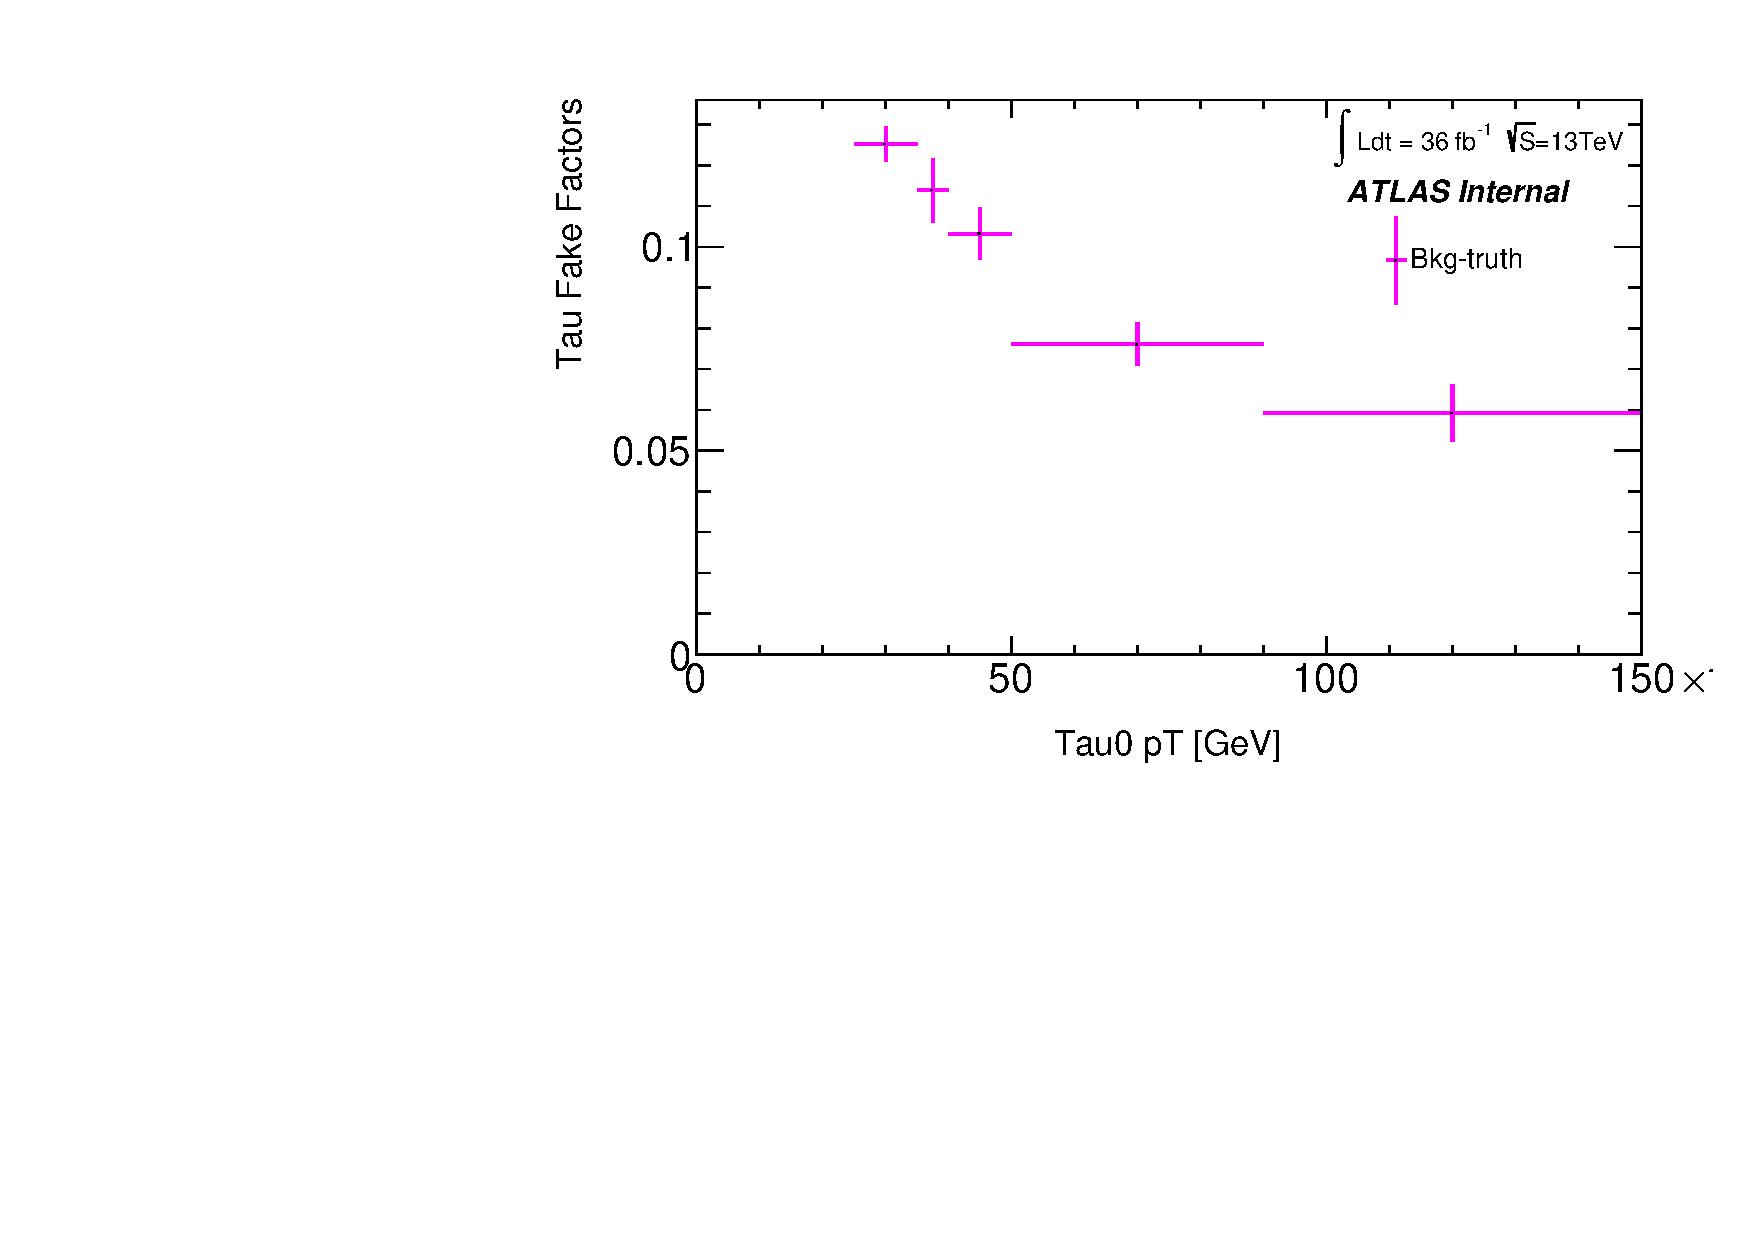
\includegraphics[width=1.\linewidth]{figures/FakesEstimate_data_pp8_nonallhad_new_SubtractionFix_newOverlay/FF_Faketau_Bkg-truth.pdf}
  	\caption{$p_T$-parametrized fake factors}
  	\label{fig:sub1}
	\end{subfigure}%
	\begin{subfigure}{.5\textwidth}
	\centering
	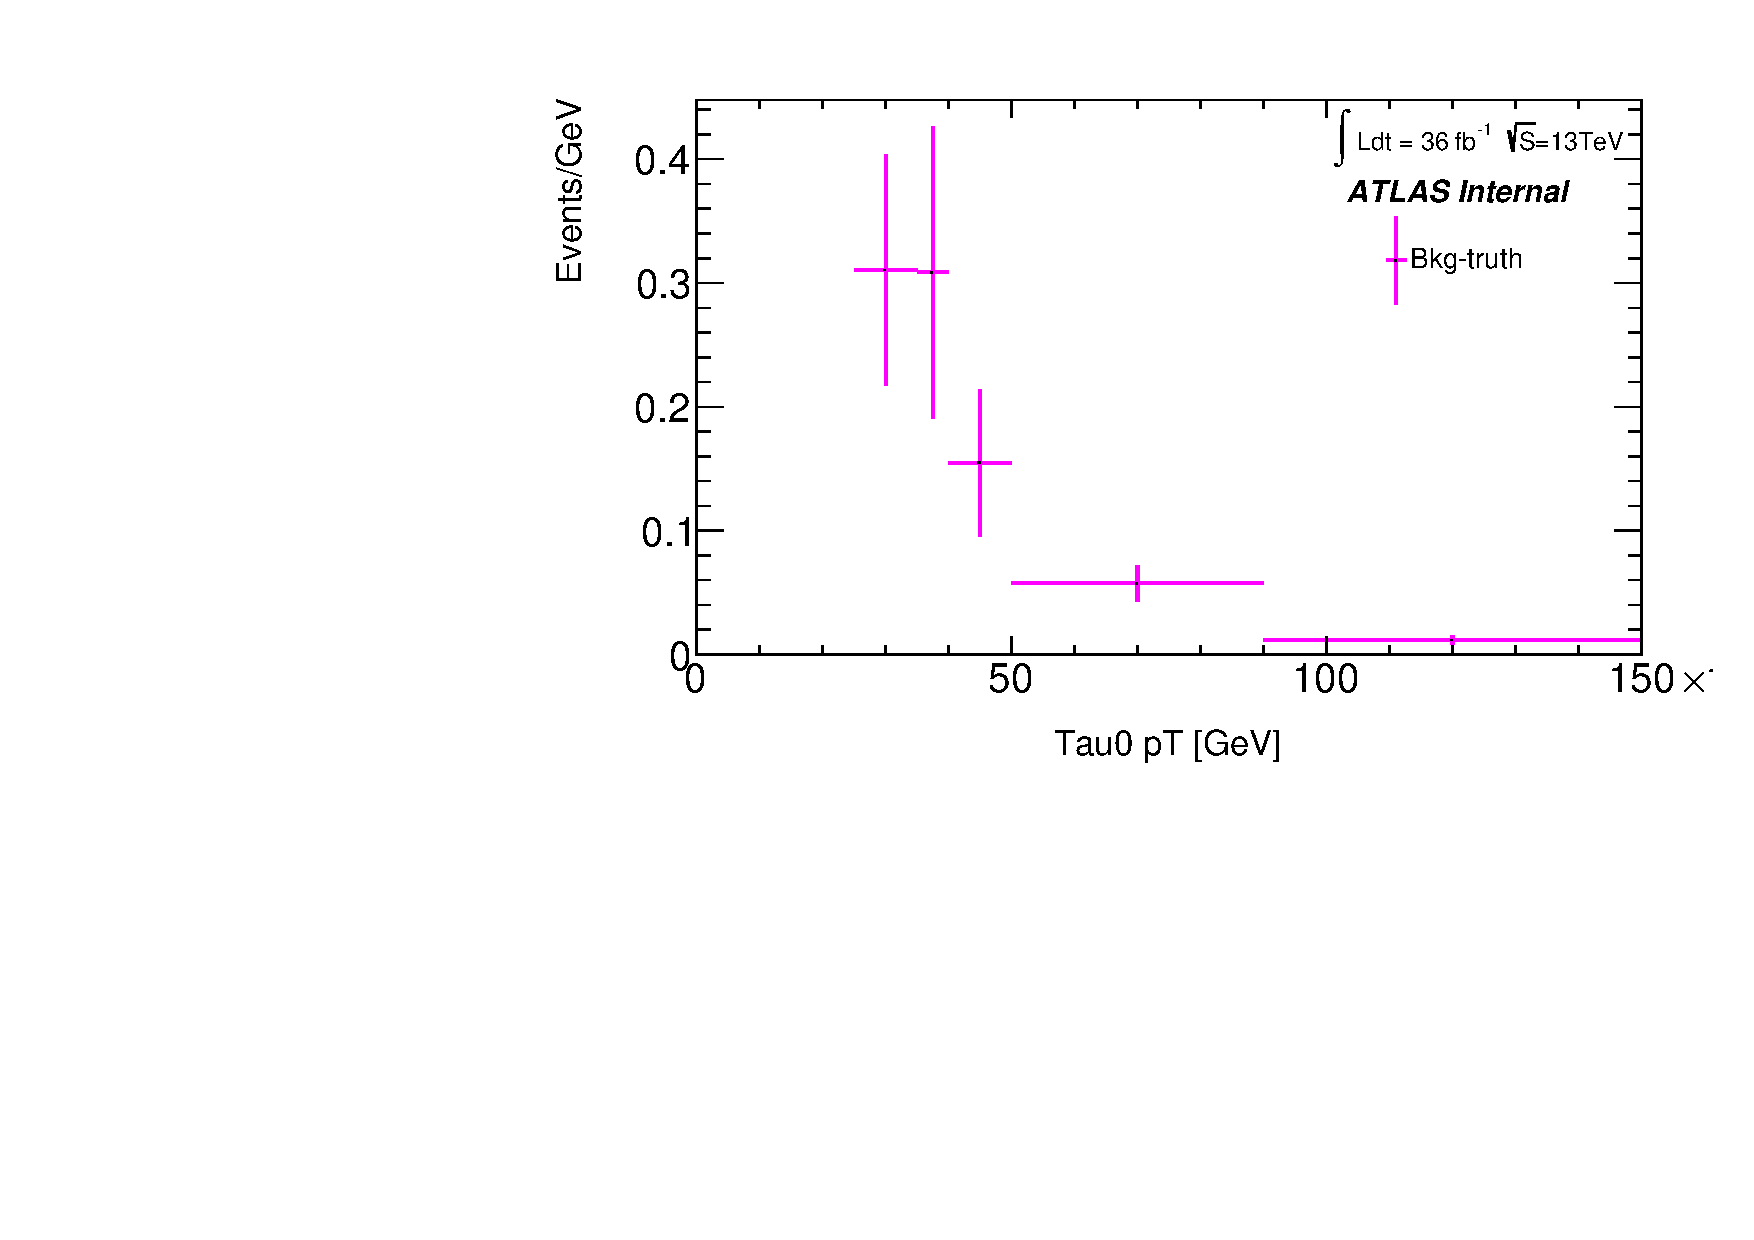
\includegraphics[width=1.\linewidth]{figures/FakesEstimate_data_pp8_nonallhad_new_SubtractionFix_newOverlay/hist_Extrapolation_Bkg-truth.pdf}
	\caption{Extrapolation sideband region $p_T$ spectrum}
	\end{subfigure}
	\caption{Fake factors and extrapolation sideband region, (All MC - Truth-matched MC - $t\bar{t}H$)}
	\end{figure}
	
	\begin{figure}[H]
	\centering
	\begin{subfigure}{.5\textwidth}
	\centering
	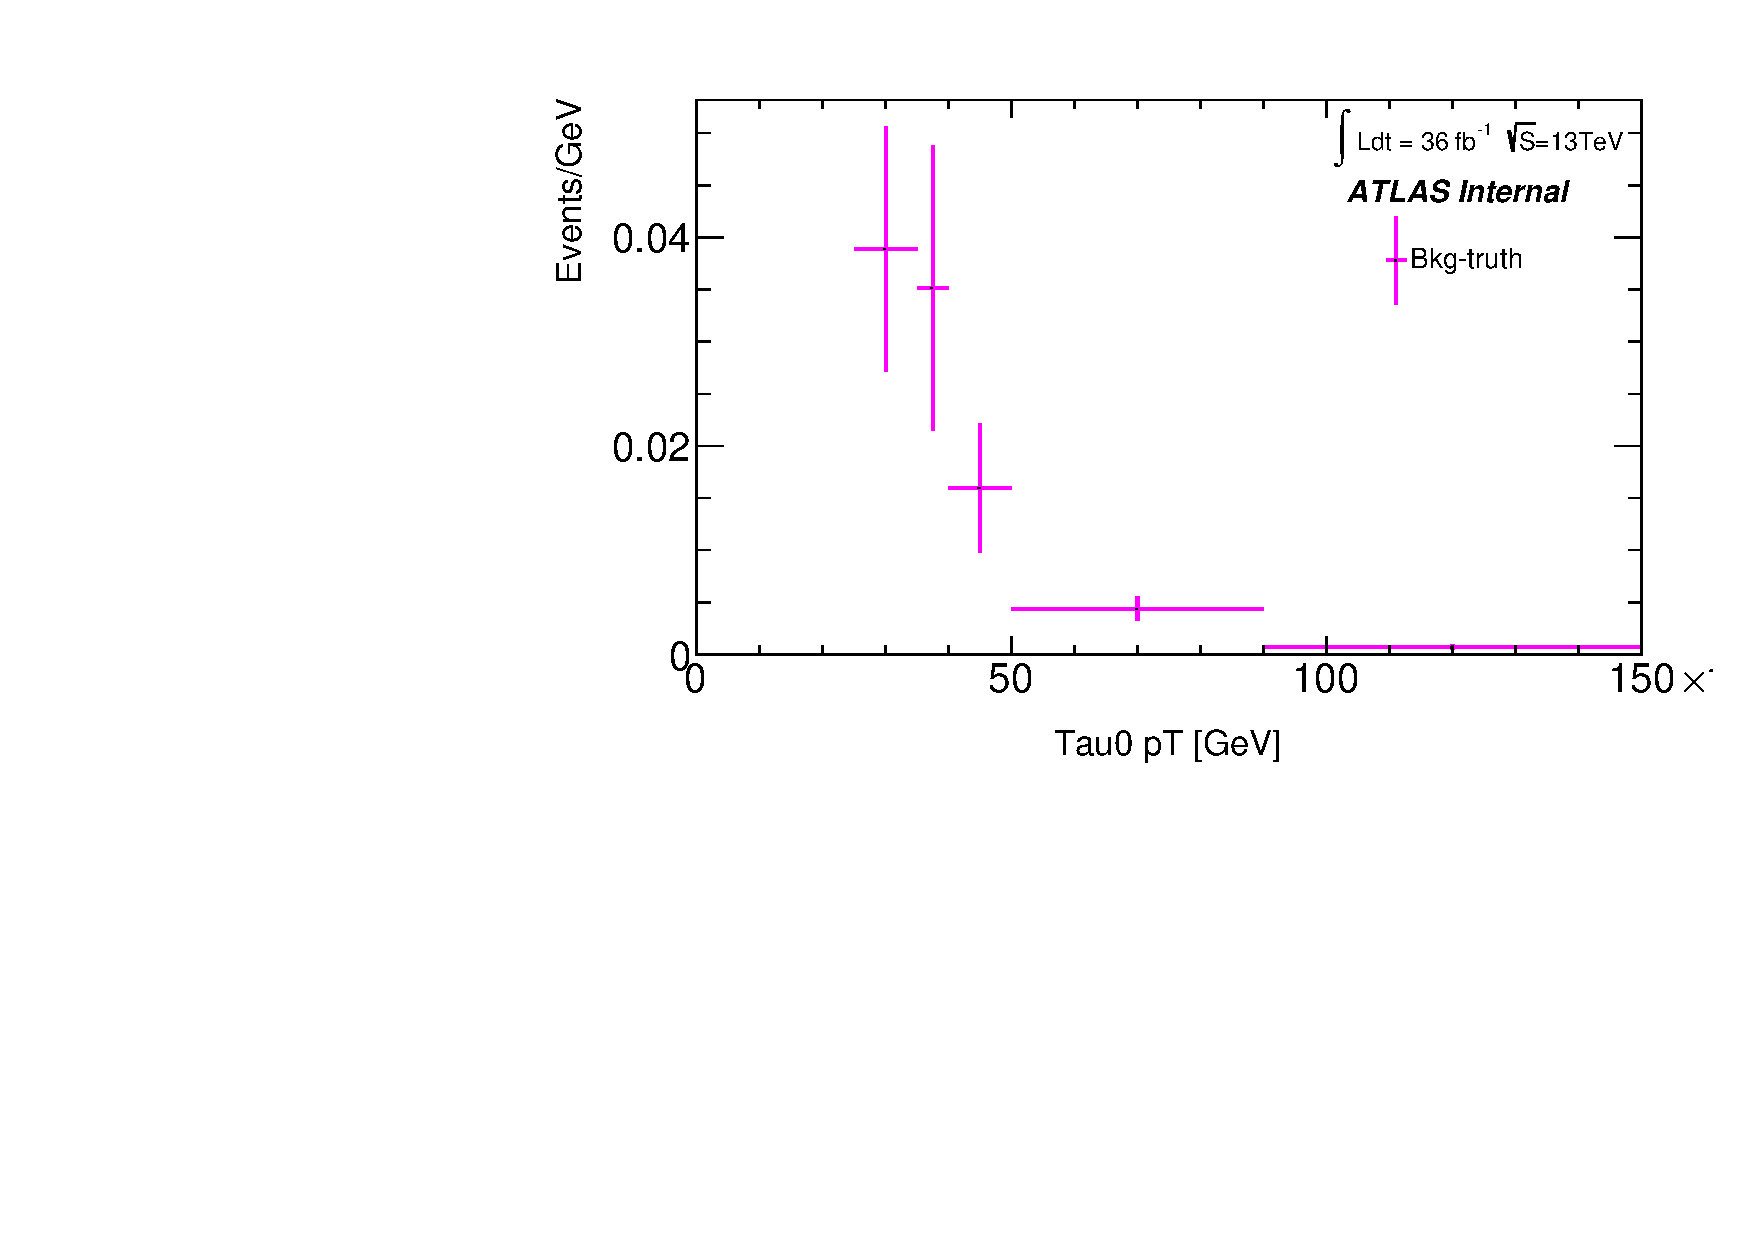
\includegraphics[width=1.\linewidth]{figures/FakesEstimate_data_pp8_nonallhad_new_SubtractionFix_newOverlay/hist_FakeEstimate_Bkg-truth.pdf}
  	\caption{Fake estimate in $p_T$ bins}
  	\label{fig:sub1}
	\end{subfigure}%
	\begin{subfigure}{.5\textwidth}
	\centering
	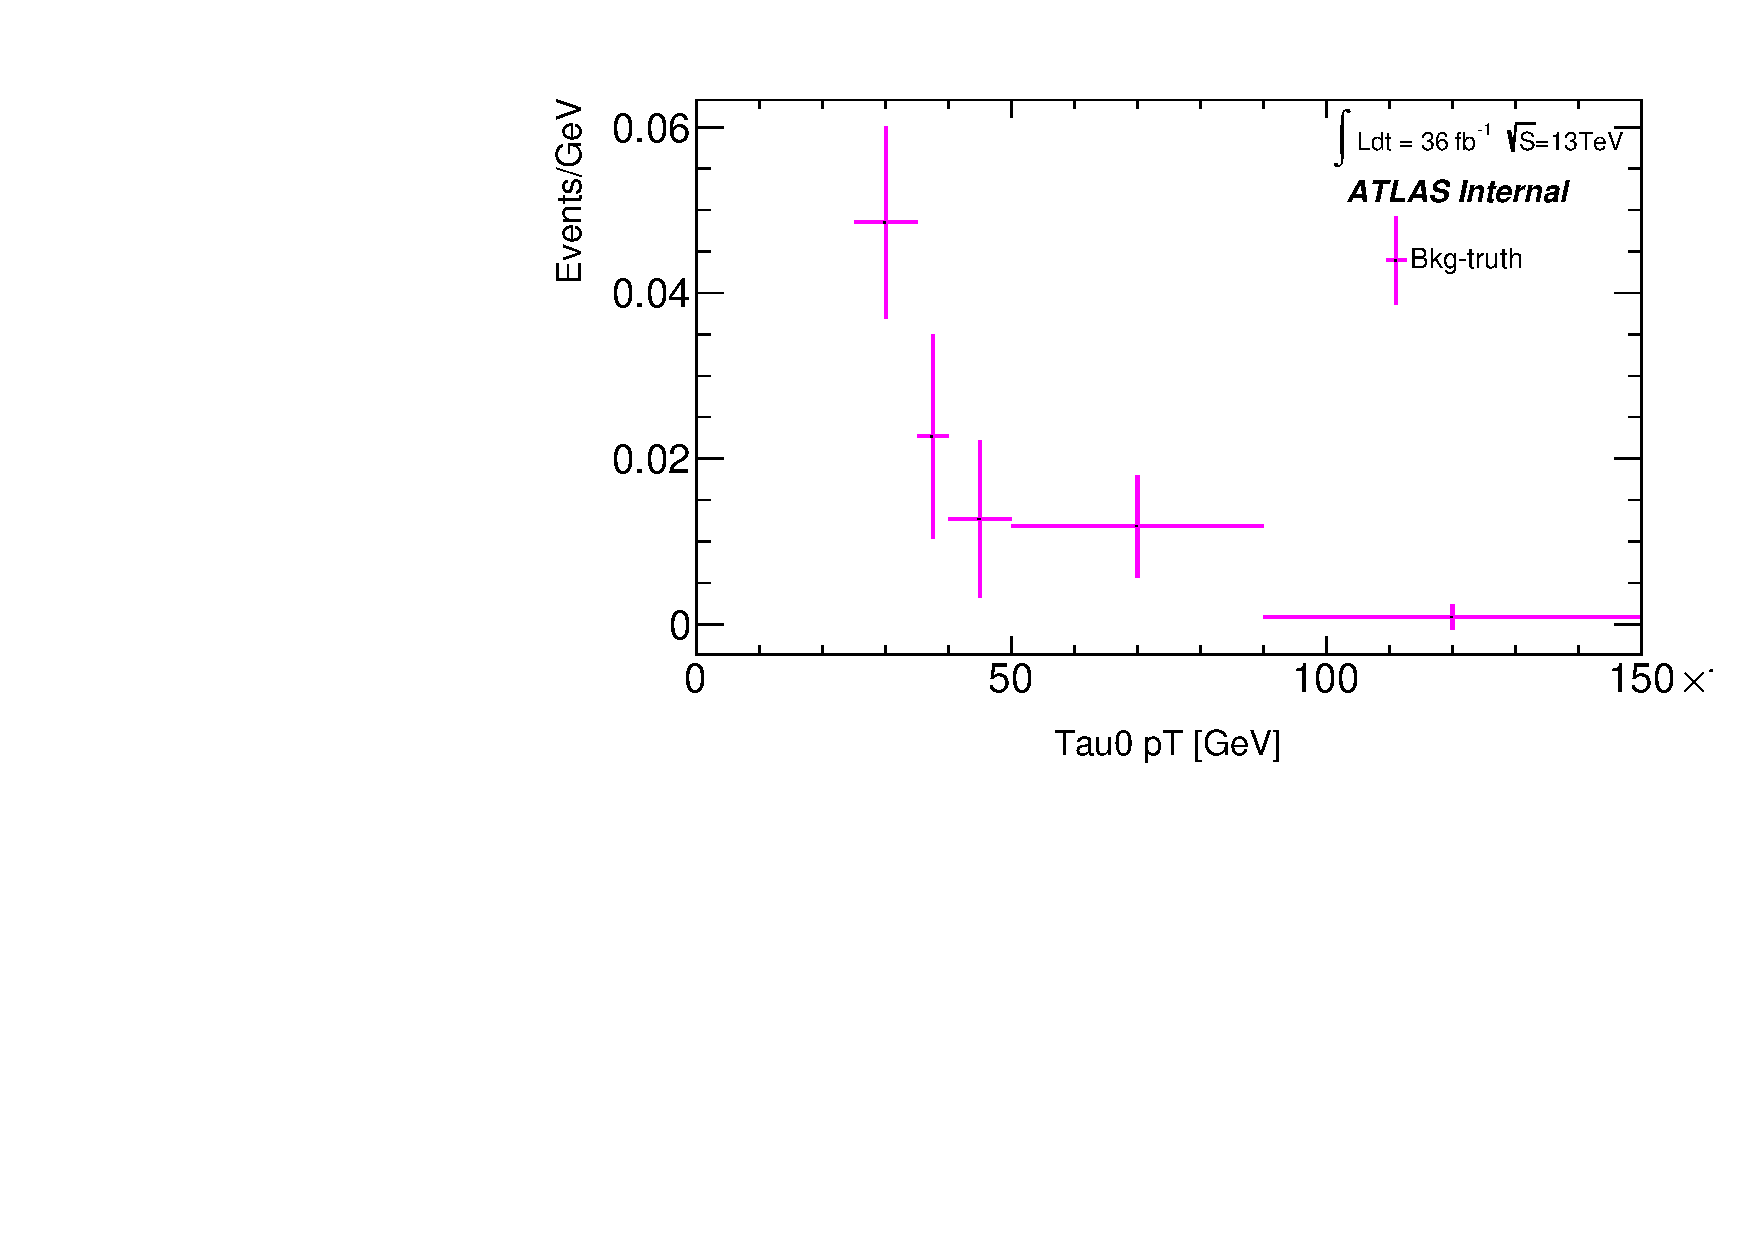
\includegraphics[width=1.\linewidth]{figures/FakesEstimate_data_pp8_nonallhad_new_SubtractionFix_newOverlay/hist_SRMC_Bkg-truth.pdf}
	\caption{MC SR yield in $p_T$ bins}
	\end{subfigure}
	\caption{$p_T$ spectra for fake estimate and MC yield, (All MC - Truth-matched MC - $t\bar{t}H$)}
	\end{figure}

	\begin{figure}[H]
		\centering
		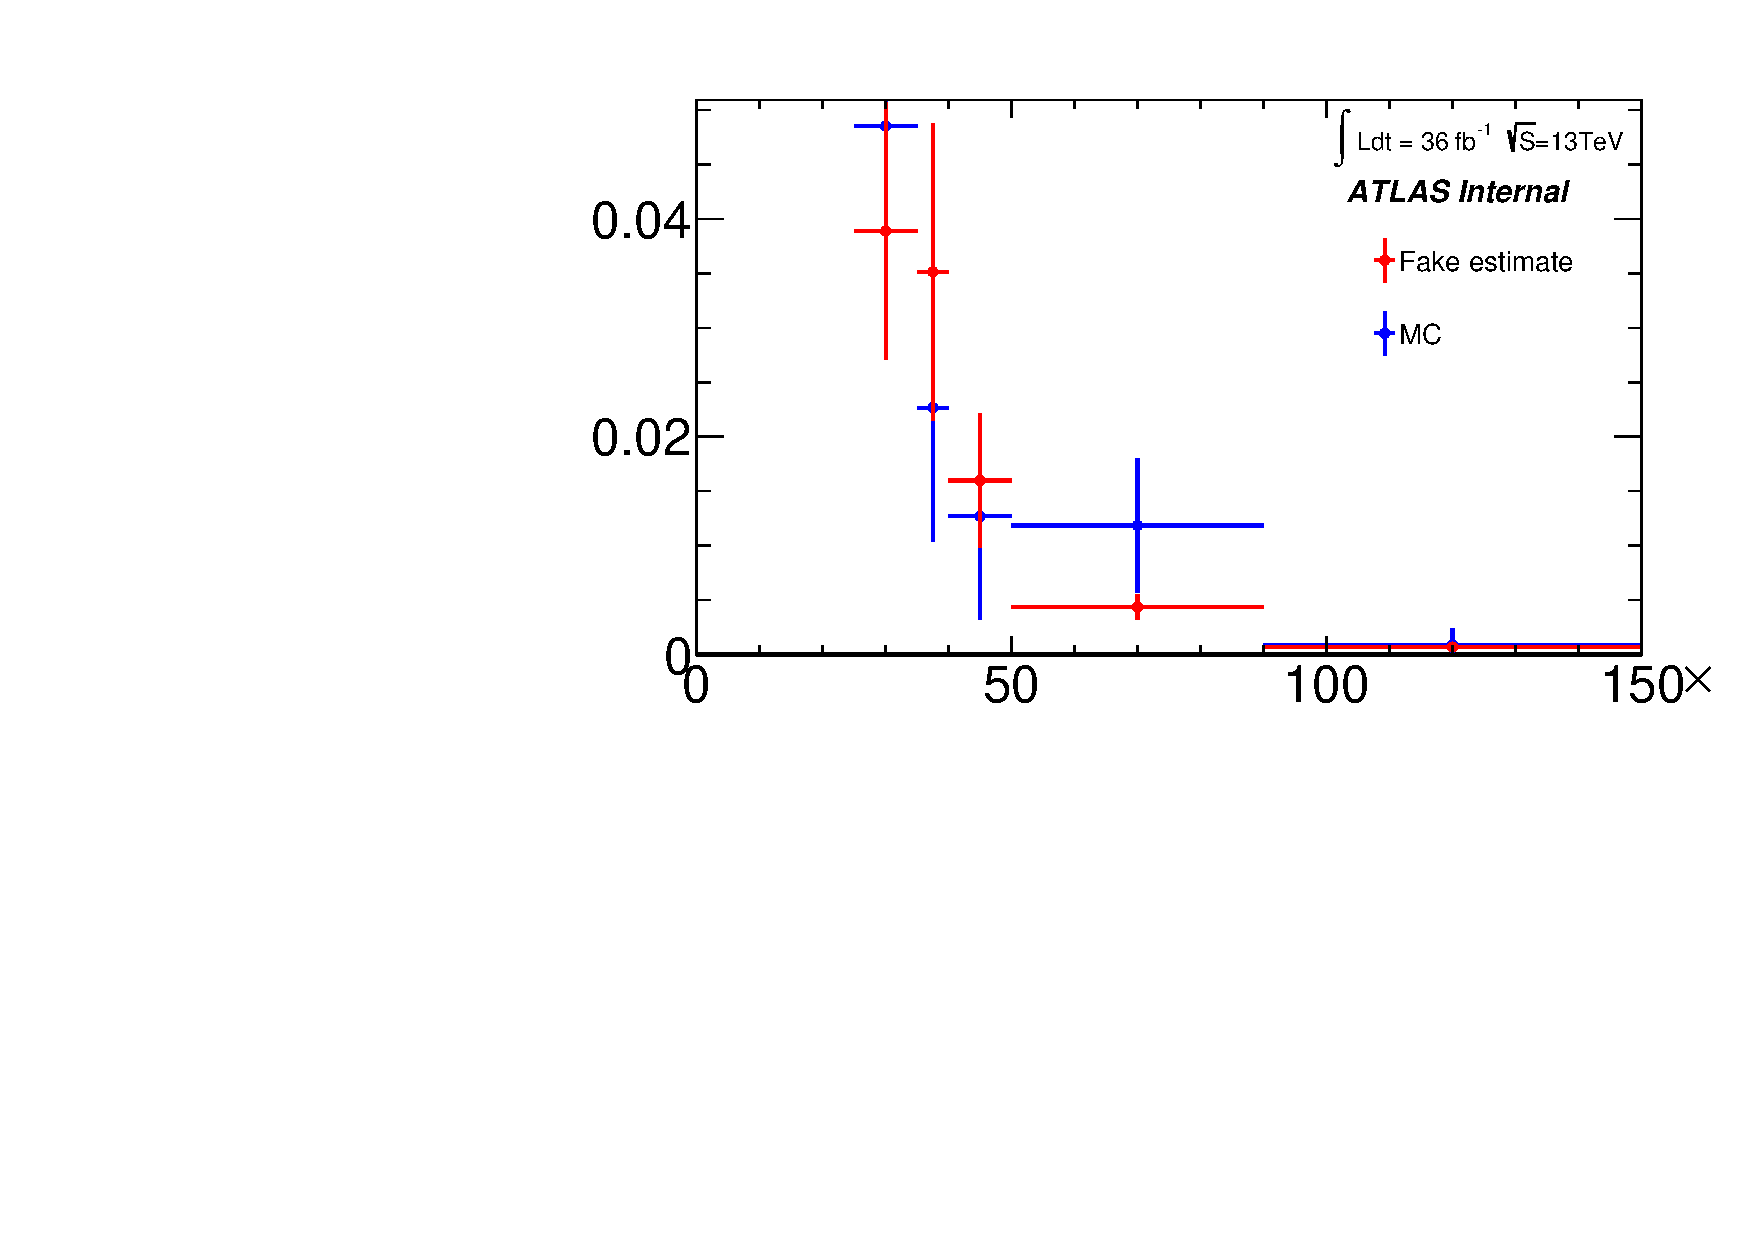
\includegraphics[width=0.7\linewidth]{figures/FakesEstimate_data_pp8_nonallhad_new_SubtractionFix_newOverlay/Overlay_FF_tau_pt_bkg.pdf}
		\caption{Overlaid fake estimate and MC prediction (All MC - Truth-matched MC - $t\bar{t}H$)}
	\end{figure}


	\begin{figure}[H]
	\centering
	\begin{subfigure}{.5\textwidth}
	\centering
	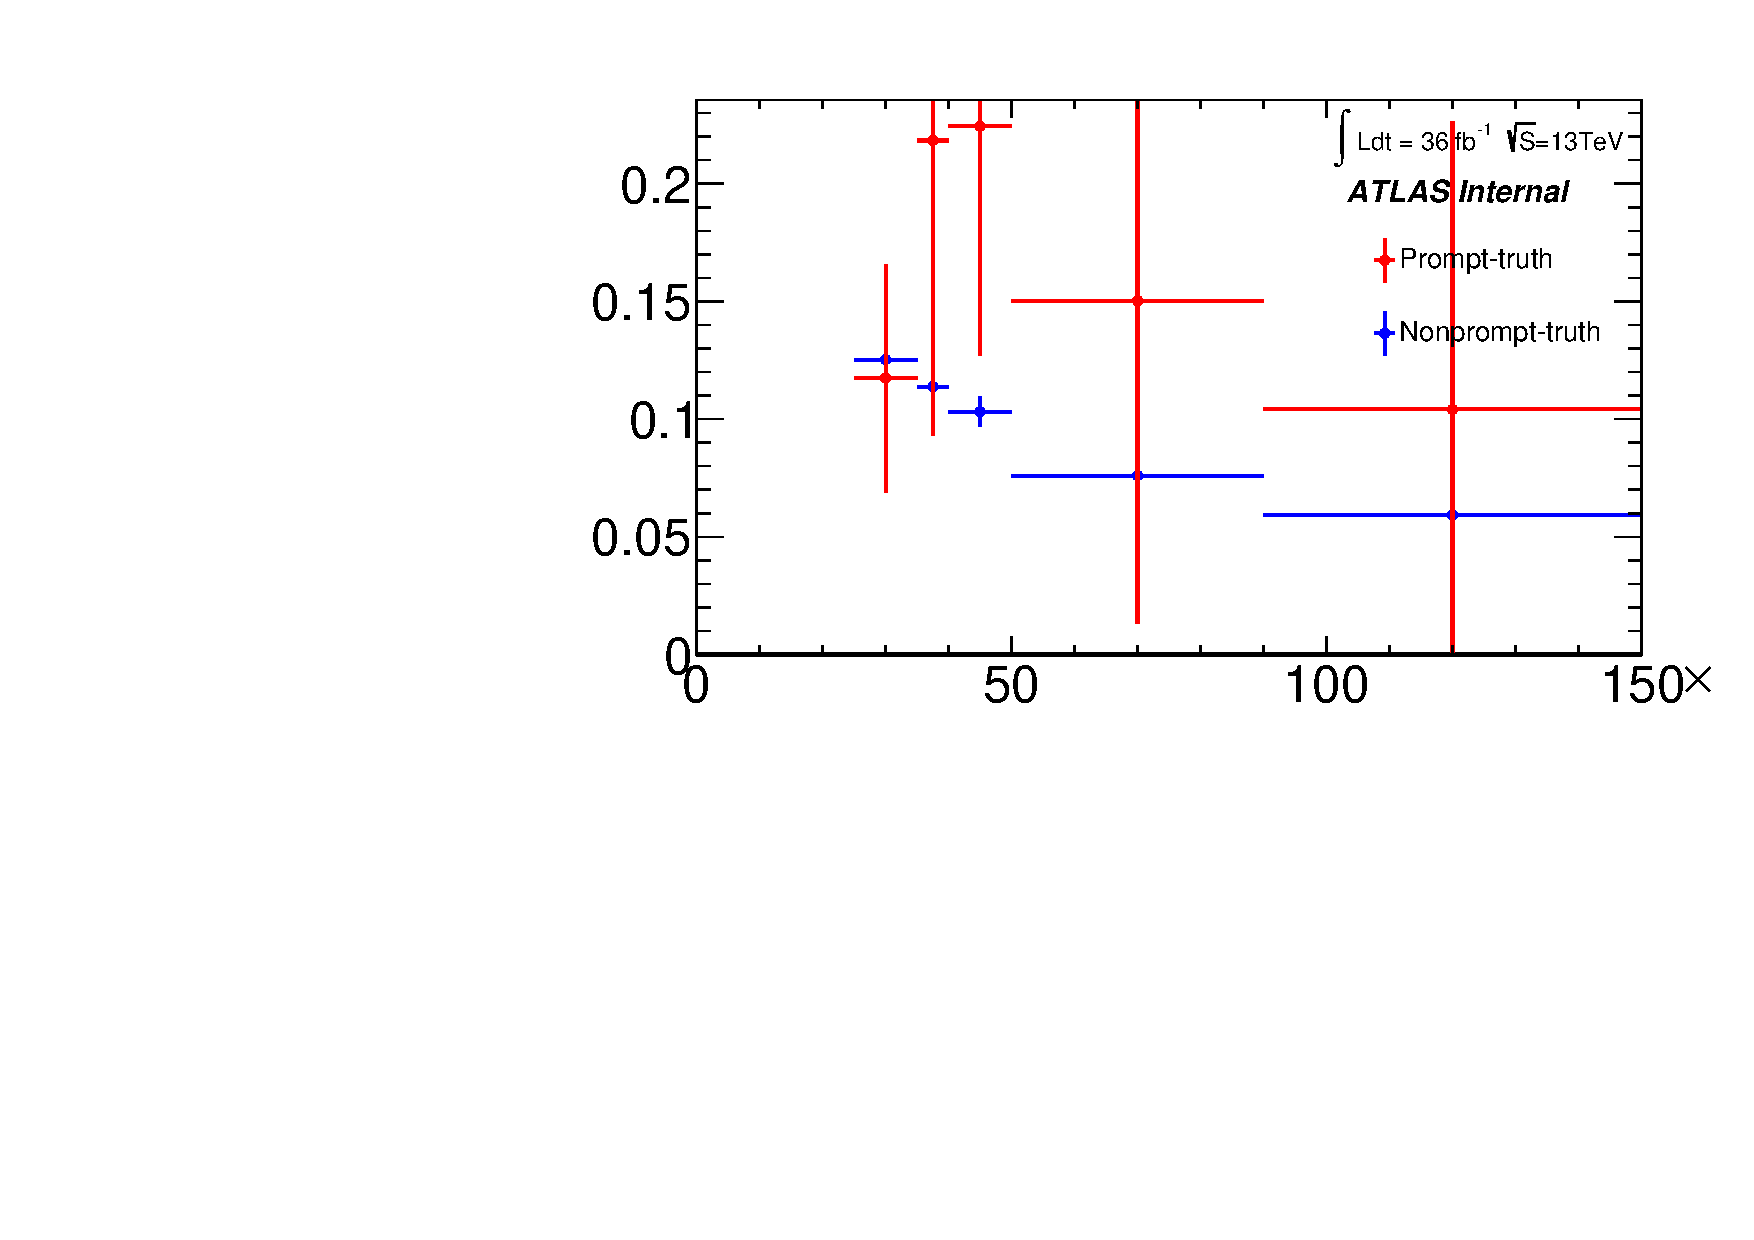
\includegraphics[width=1.\linewidth]{figures/FakesEstimate_data_pp8_nonallhad_new_SubtractionFix_newOverlay/Overlay_FF_CompareFF_prompt_nonprompt.pdf}
  	\caption{Prompt (red) and non-prompt (blue)  }
  	\label{fig:sub1}
	\end{subfigure}%
	\begin{subfigure}{.5\textwidth}
	\centering
	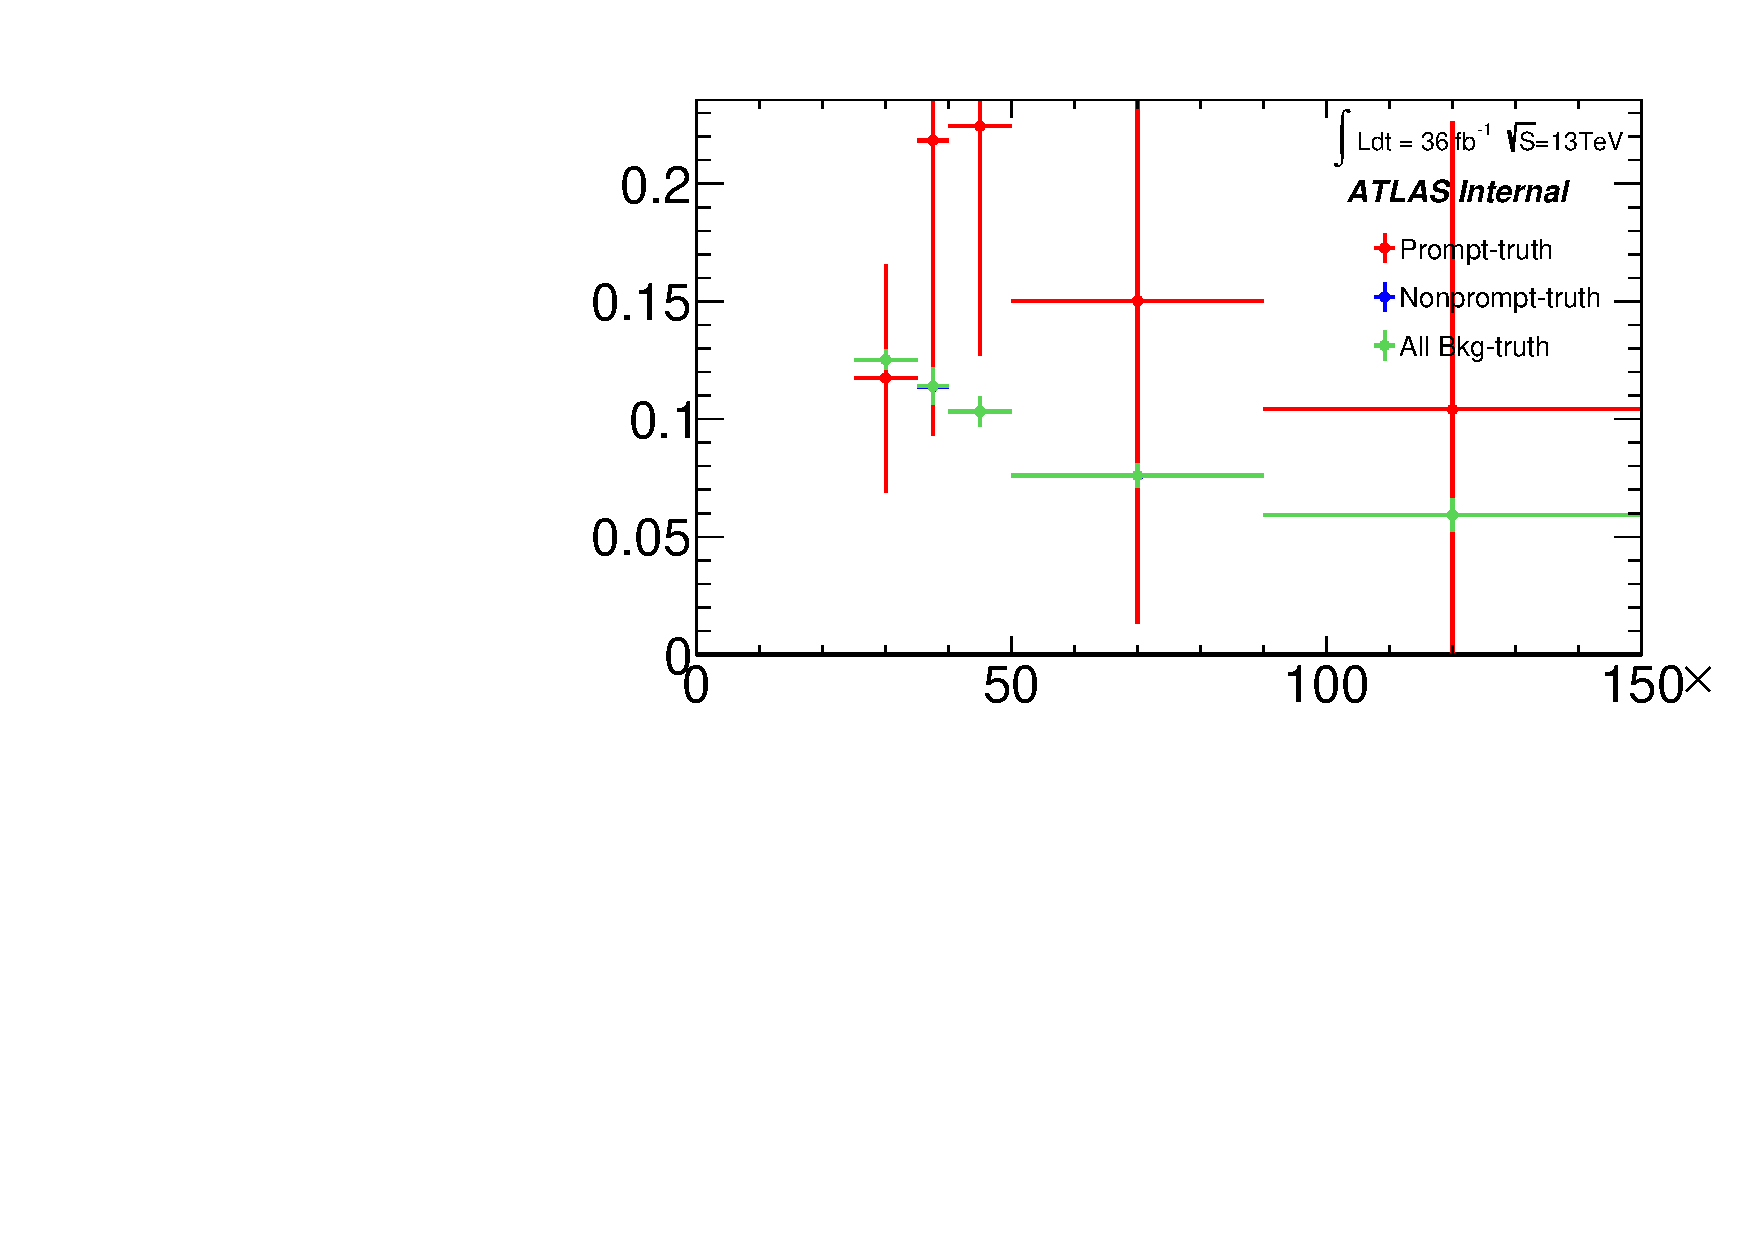
\includegraphics[width=1.\linewidth]{figures/FakesEstimate_data_pp8_nonallhad_new_SubtractionFix_newOverlay/Overlay_FF_CompareFF_all.pdf}
	\caption{Prompt, non-prompt and combined (green) }
	\end{subfigure}
	\caption{Comparison of fake factors derived from prompt MC, non-prompt MC and from the full combined (prompt + non-prompt - truth) method}
	\end{figure}
	
			
		
		
	\clearpage
	\subsection{Estimate with non-prompt MC - truth-matched} 
	\begin{equation}
		FF(p_T)_{MC} = \frac{N_\tau (p_T)^{\text{Non-prompt MC}} - N_\tau (p_T)^{\text{Truth-matched non-prompt MC}}}{N_{\cancel{\tau}} (p_T)^{\text{Non-prompt MC}} - N_{\cancel{\tau}} (p_T)^{\text{Truth-matched non-prompt MC}}}
	\end{equation}

	\begin{table}[htp]
	\caption{Extrapolation and closure test, (Non-prompt MC - truth-matched)}
	\begin{center}
	\begin{tabular}{|c|c|c|c|c|}
	\hline
	$t\bar{t}$ sample 	& Integrated fake estimate	& SR MC		&  	Raw, total ($t\bar{t}$) 	& Closure \\
	\hline
	PP8 non-all hadronic			& 	$0.574\pm0.143$ 		& $0.587\pm0.406$ 		& 138 (1)	&  $2\pm75$\% \\
	PP8 non-all hadronic, high stats	& 	$0.646\pm0.128$ 		& $0.393\pm0.215$ 		& 138 (1)	&  $-39\pm35$\% \\
	PP8 dilepton 					& 	$0.442\pm0.104$ 		& $0.414\pm0.236$ 		& 138 (1)	&  $-6\pm58$\% \\
	PP8 dilepton, high stats			& 	$0.519\pm0.088$ 		& $0.588\pm0.242$ 		& 140 (3)	&  $13\pm51$\% \\
	\hline
	\end{tabular}
	\end{center}
	\label{default}
	\end{table}%
		
	Figures are produced using the non-all hadronic high-stats sample. 
		
	\begin{figure}[H]
	\centering
	\begin{subfigure}{.5\textwidth}
	\centering
	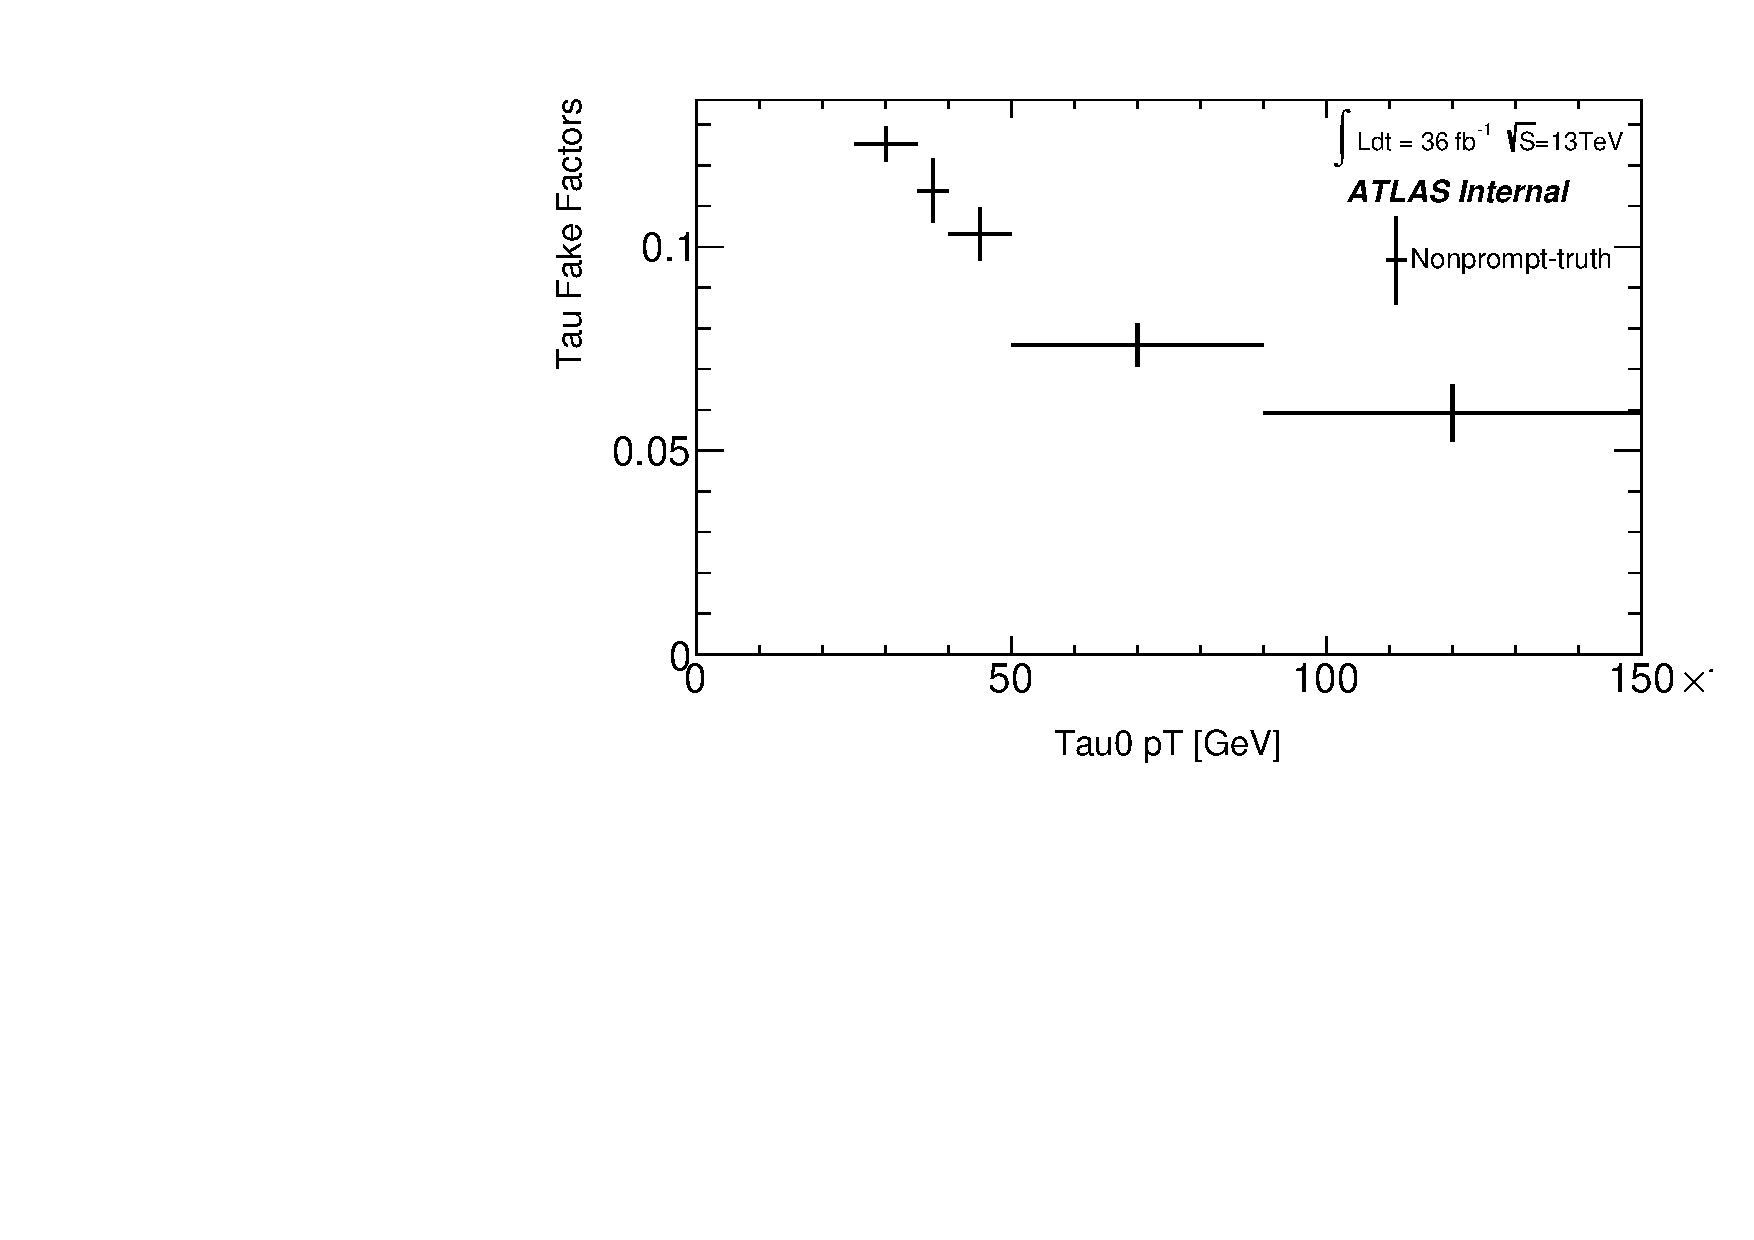
\includegraphics[width=0.95\linewidth]{figures/FakesEstimate_data_pp8_nonallhad_new_scaledHists/FF_Faketau_Nonprompt-truth.pdf}
  	\caption{$p_T$-parametrized fake factors}
  	\label{fig:sub1}
	\end{subfigure}%
	\begin{subfigure}{.5\textwidth}
	\centering
	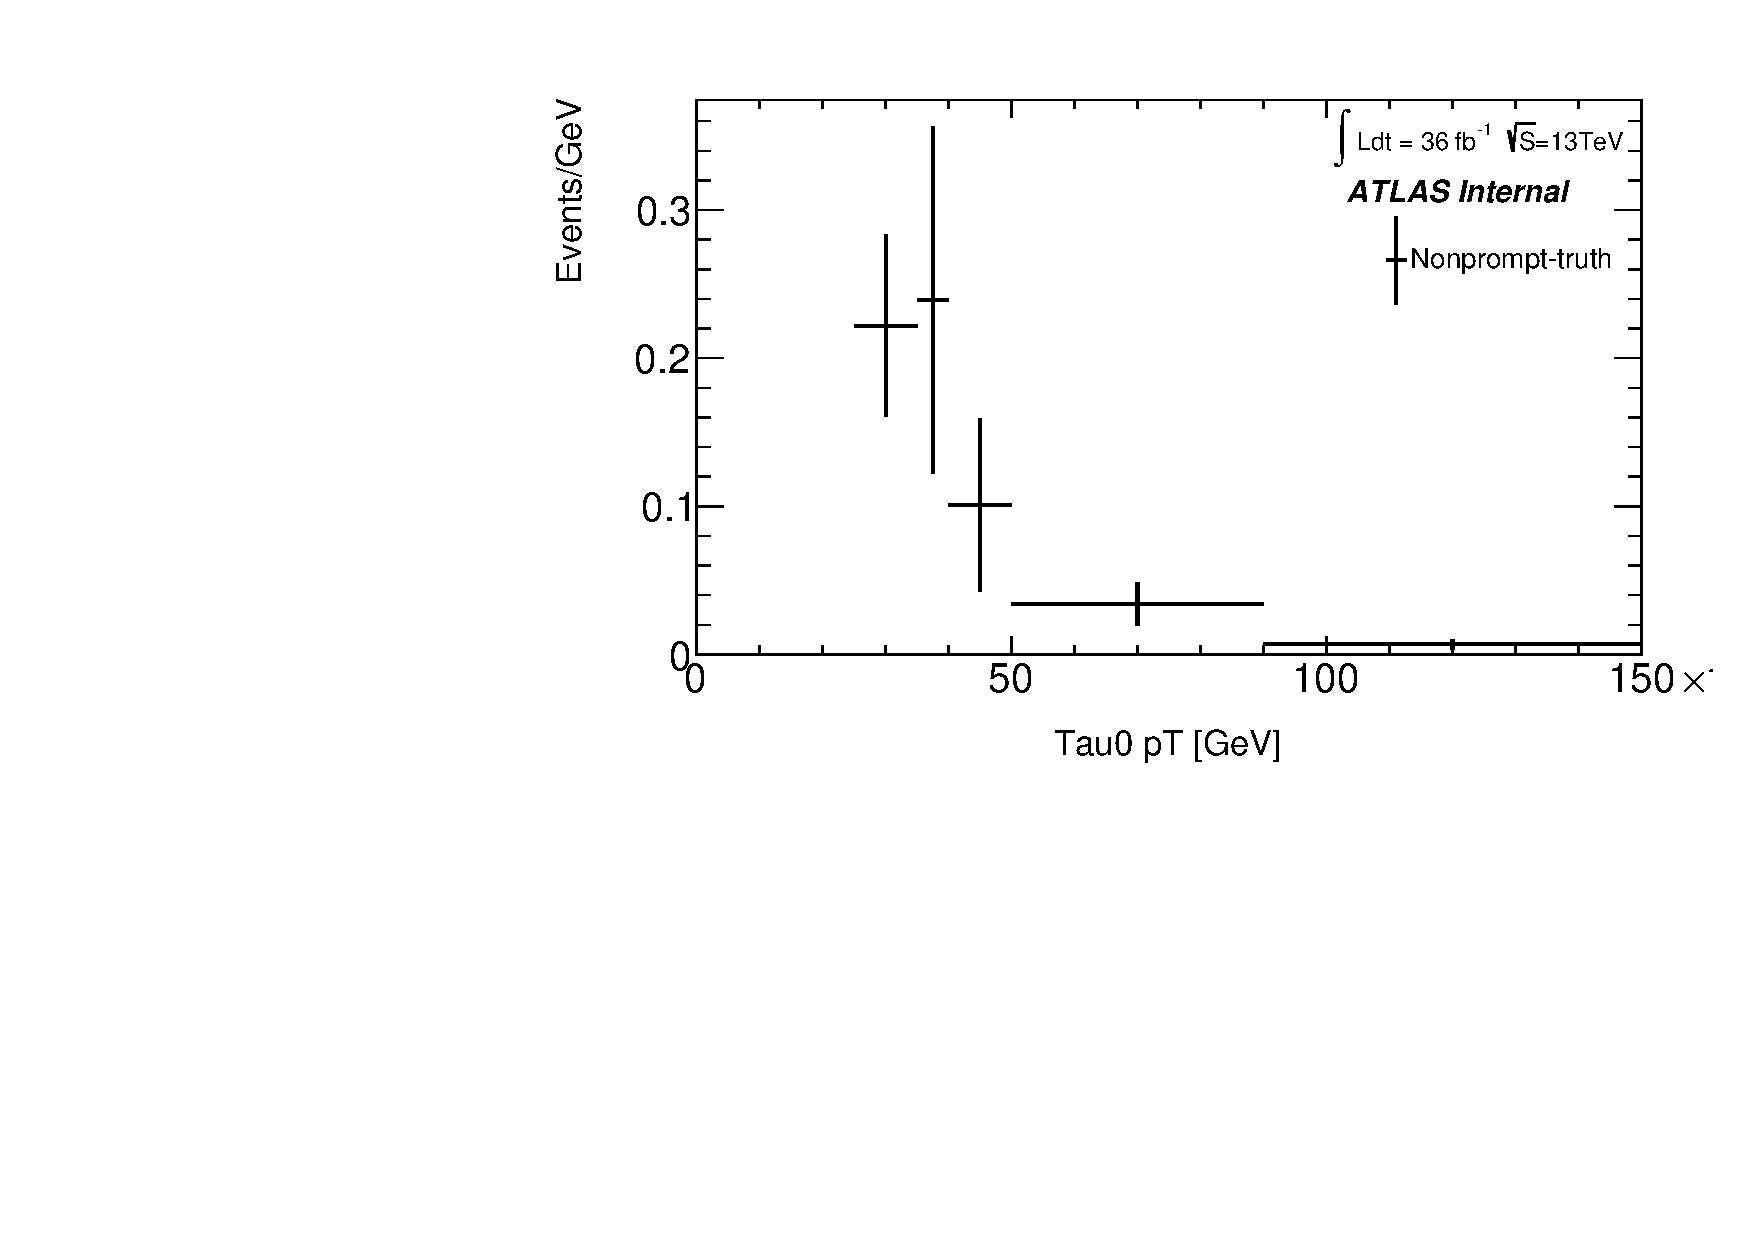
\includegraphics[width=0.95\linewidth]{figures/FakesEstimate_data_pp8_nonallhad_new_scaledHists/hist_Extrapolation_Nonprompt-truth.pdf}
	\caption{Extrapolation sideband region $p_T$ spectrum}
	\end{subfigure}
	\caption{Fake factors and extrapolation sideband region, (Non-prompt MC - truth)}
	\end{figure}
	
	\begin{figure}[H]
	\centering
	\begin{subfigure}{.5\textwidth}
	\centering
	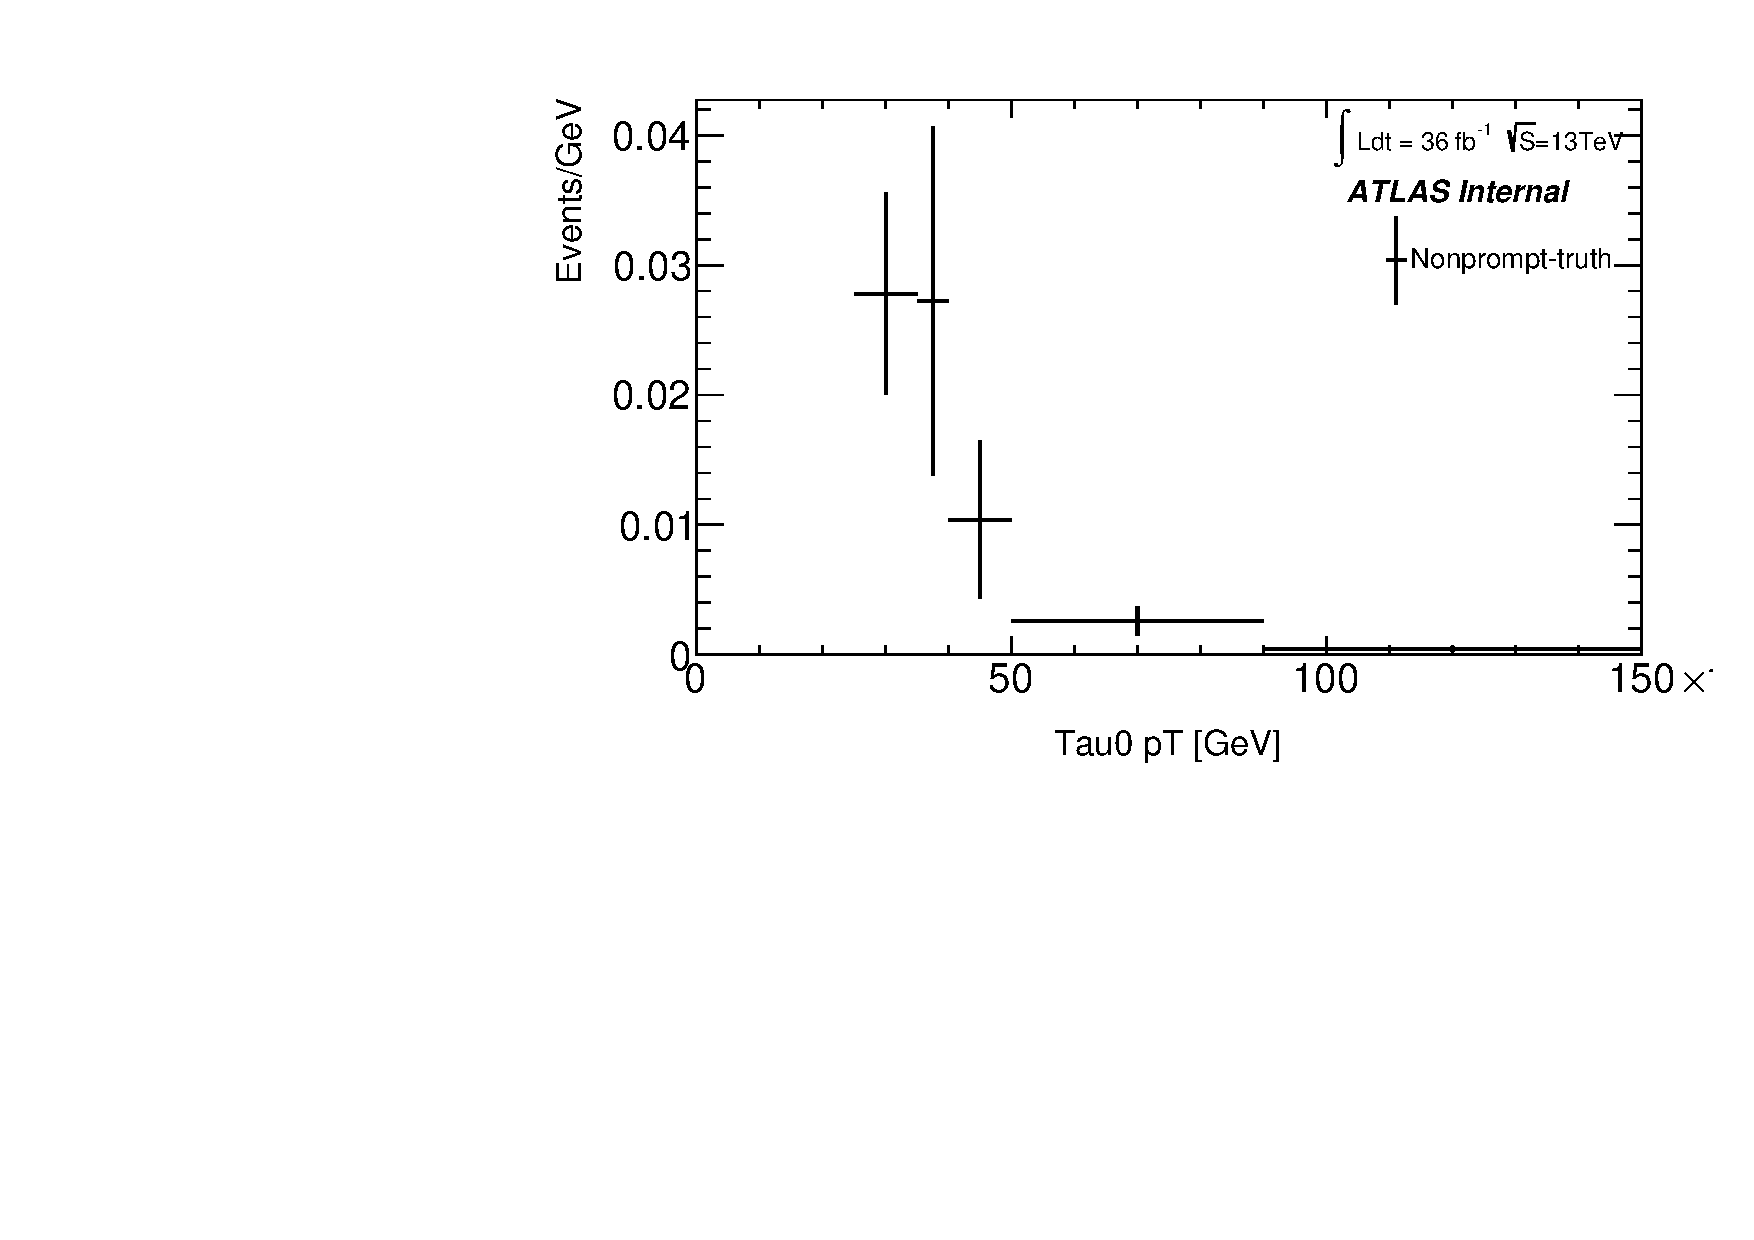
\includegraphics[width=0.95\linewidth]{figures/FakesEstimate_data_pp8_nonallhad_new_scaledHists/hist_FakeEstimate_Nonprompt-truth.pdf}
  	\caption{Fake estimate in $p_T$ bins}
  	\label{fig:sub1}
	\end{subfigure}%
	\begin{subfigure}{.5\textwidth}
	\centering
	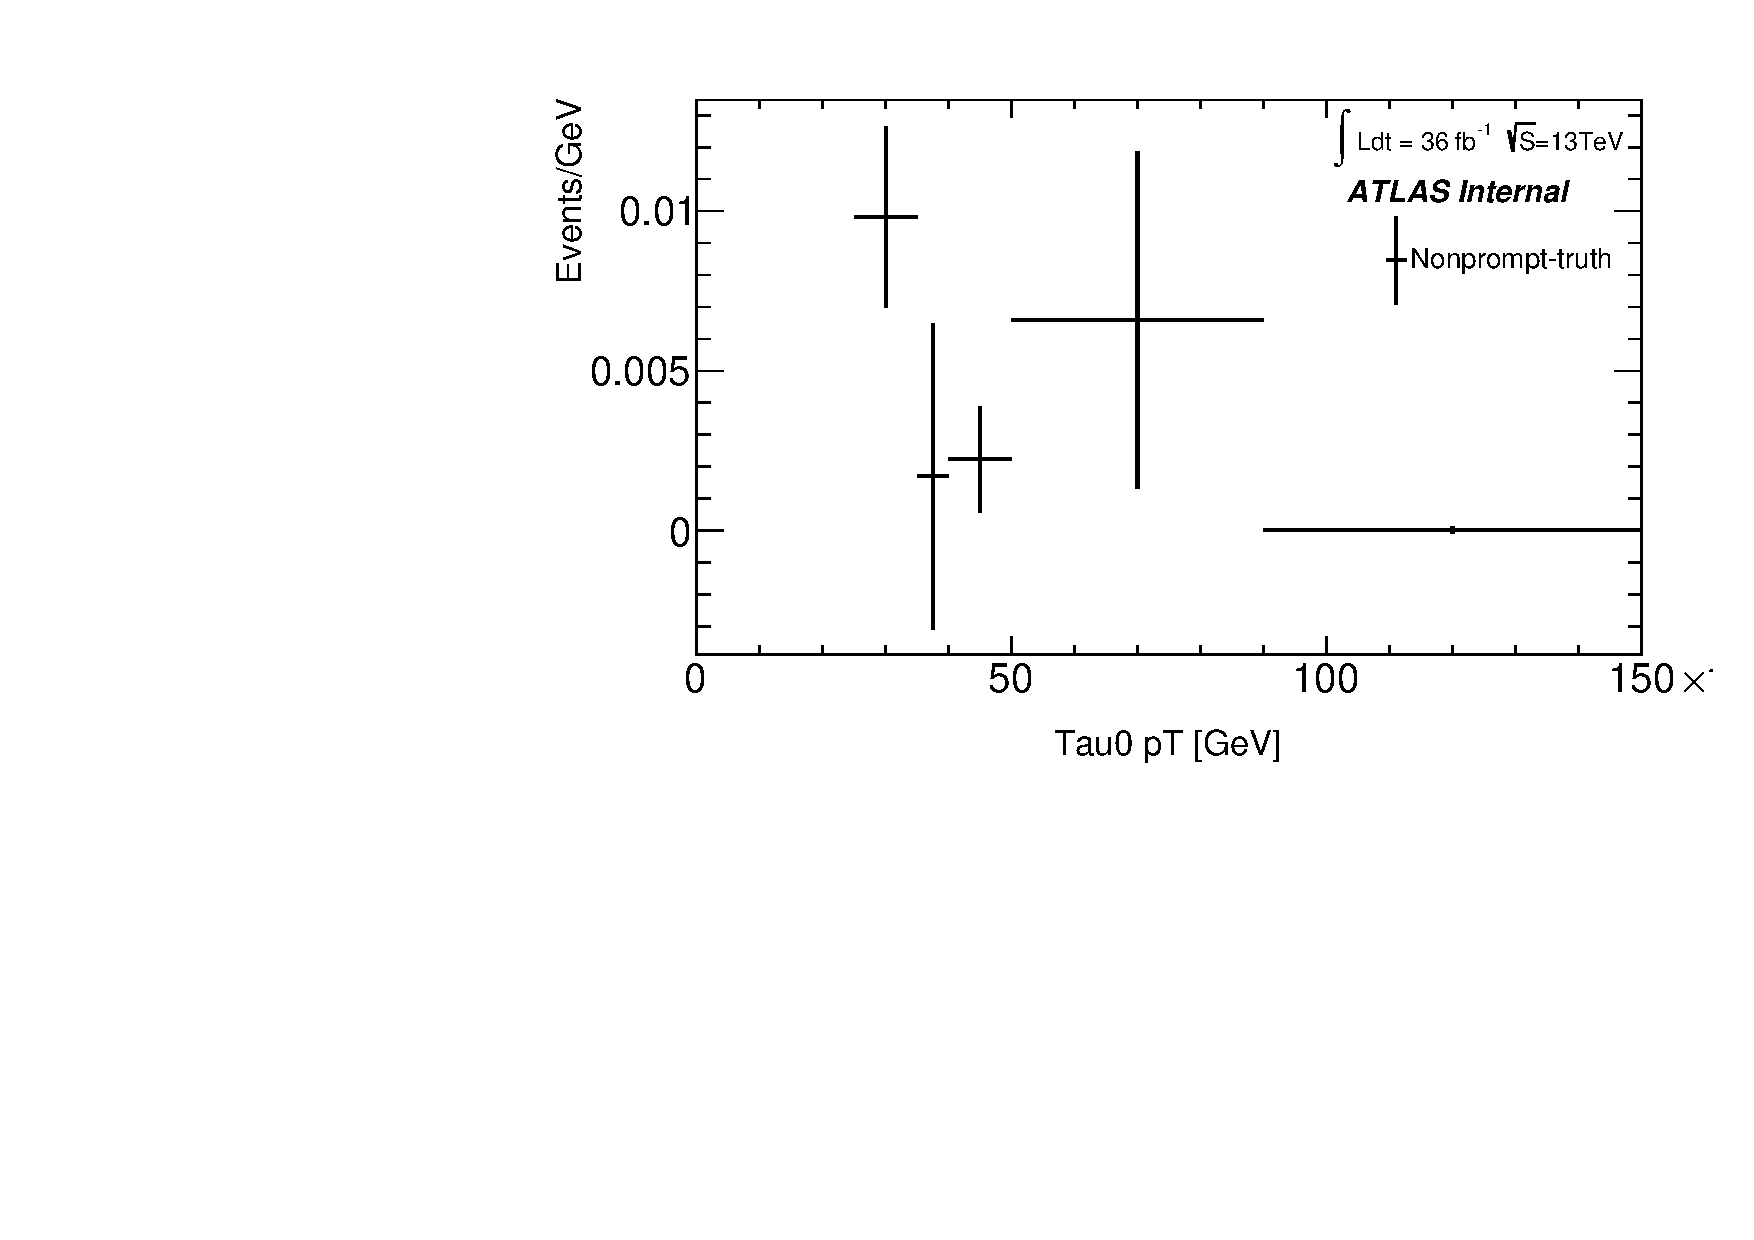
\includegraphics[width=0.95\linewidth]{figures/FakesEstimate_data_pp8_nonallhad_new_scaledHists/hist_SRMC_Nonprompt-truth.pdf}
	\caption{MC SR yield in $p_T$ bins}
	\end{subfigure}
	\caption{$p_T$ spectra for fake estimate and MC yield, (Non-prompt MC - truth)}
	\end{figure}

	\begin{figure}[H]
		\centering
		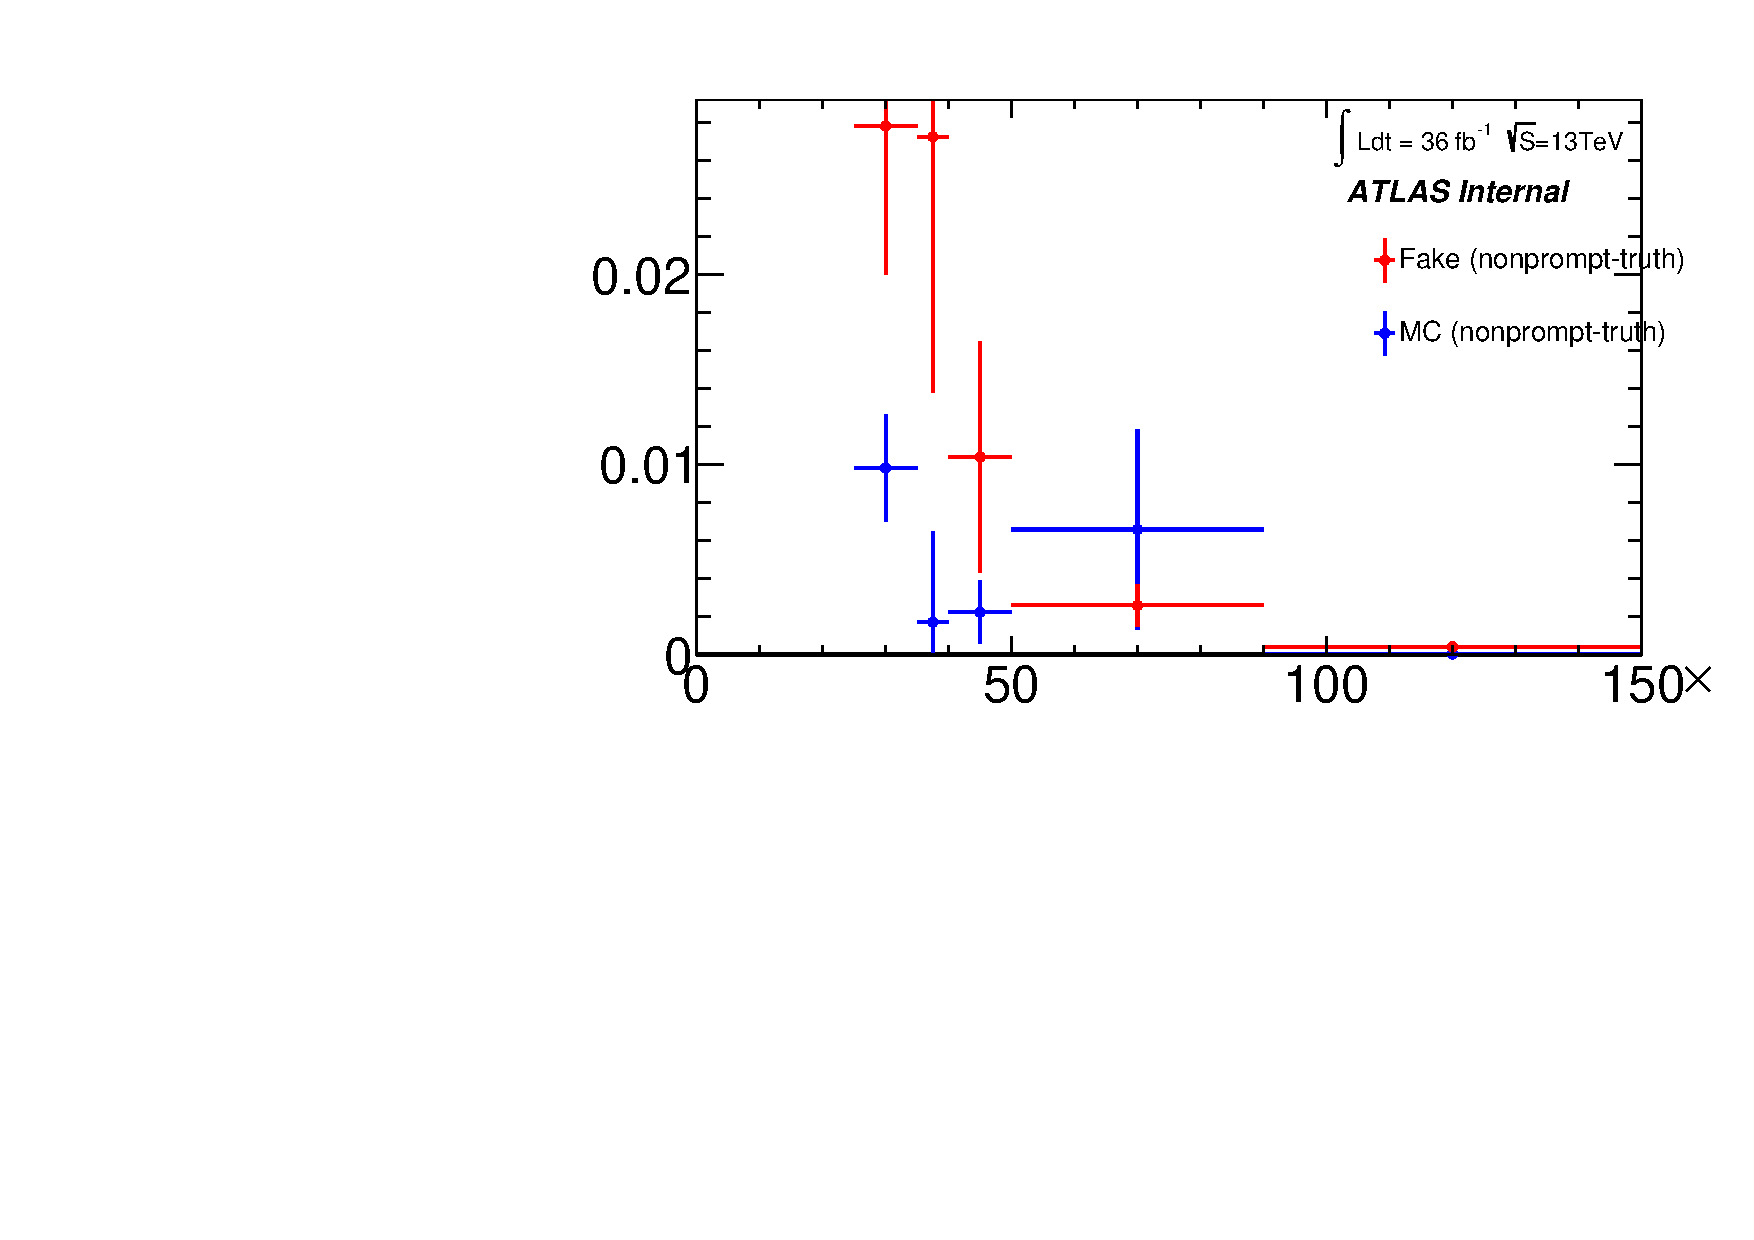
\includegraphics[width=0.7\linewidth]{figures/FakesEstimate_data_pp8_nonallhad_new_scaledHists/Overlay_FF_tau_pt_nonprompt-truth.pdf}
		\caption{Overlaid fake estimate and MC prediction (Non-prompt MC - truth)}
	\end{figure}	

		\begin{table}[htp]
		\caption{Raw yield comparison for signal region comparing low-stats $t\bar{t}$ non-all hadronic and dilepton low-stats samples}
		\resizebox{1.0\textwidth}{!}{
 		\begin{tabular}{|c|c|c|c|c|c|}
 		\hline
 			              & ttH                        & Prompt bkg                 & Nonprompt bkg (no ttbar)                 & ttbar non-all hadronic                     & ttbar dilepton                               \\
		\hline
		Input            & $7196834.000 \pm 2682.692$ & $5923407.000 \pm 2433.805$ & $155015314.000 \pm 12450.515$ & $11452200.000 \pm 3384.110$ & $6562556.000 \pm 2561.749$ \\
 		CutBlind         & $7196834.000 \pm 2682.692$ & $5923407.000 \pm 2433.805$ & $155015314.000 \pm 12450.515$ & $11452200.000 \pm 3384.110$ & $6562556.000 \pm 2561.749$ \\
		Cleaning         & $7196834.000 \pm 2682.692$ & $5923407.000 \pm 2433.805$ & $155015314.000 \pm 12450.515$ & $11452200.000 \pm 3384.110$ & $6562556.000 \pm 2561.749$ \\
		CutSLORDLTrigger & $5124841.000 \pm 2263.811$ & $4621965.000 \pm 2149.876$ & $120080497.000 \pm 10958.125$ &  $7944424.000 \pm 2818.585$ & $5279307.000 \pm 2297.674$ \\
		Cut3Leptons      &   $247338.000 \pm 497.331$ &   $770943.000 \pm 878.034$ &    $1235939.000 \pm 1111.728$ &     $51759.000 \pm 227.506$ &    $80321.000 \pm 283.410$\\
 		CutLepTightMVA   &   $103371.000 \pm 321.514$ &   $466468.000 \pm 682.985$ &      $574917.000 \pm 758.233$ &        $996.000 \pm 31.559$ &      $1639.000 \pm 40.485$ \\
		CutTrigFlat      &   $102924.000 \pm 320.818$ &   $465119.000 \pm 681.996$ &      $574130.000 \pm 757.714$ &        $987.000 \pm 31.417$ &      $1624.000     \pm 40.299$    \\
		CutZCandVeto     &    $88789.000 \pm 297.975$ &   $121906.000 \pm 349.150$ &      $105100.000 \pm 324.191$ &        $869.000 \pm 29.479$ &      $1409.000     \pm 37.537$  \\
		CutLowMass12     &    $87981.000 \pm 296.616$ &   $115654.000 \pm 340.079$ &      $102436.000 \pm 320.056$ &        $849.000 \pm 29.138$ &      $1390.000     \pm 37.283$   \\
		CutNTau          &      $5888.000 \pm 76.733$ &      $4825.000 \pm 69.462$ &          $896.000 \pm 29.933$ &           $4.000 \pm 2.000$ &          $4.000     \pm 2.000$\\
		Cut3LepCharge    &      $5519.000 \pm 74.290$ &      $4080.000 \pm 63.875$ &          $613.000 \pm 24.759$ &           $4.000 \pm 2.000$ &          $3.000     \pm 1.732$ \\
		CutNJet          &      $4991.000 \pm 70.647$ &      $3004.000 \pm 54.809$ &          $356.000 \pm 18.868$ &           $2.000 \pm 1.414$ &          $1.000     \pm 1.000$ \\
 		Cut1BTag         &      $4113.000 \pm 64.133$ &      $2173.000 \pm 46.615$ &          $237.000 \pm 15.395$ &           $1.000 \pm 1.000$ &          $1.000     \pm 1.000$ \\
 		CutTauTruthMatch &      $3627.000 \pm 60.225$ &      $1354.000 \pm 36.797$ &          $100.000 \pm 10.000$ &           $0.000 \pm 0.000$ &          $0.000     \pm 0.000$ \\
 		\hline
 		\end{tabular}}
	\end{table}
		
	\begin{table}[htp]
		\caption{Raw yield comparison for signal region comparing low-stats $t\bar{t}$ non-all hadronic and dilepton high-stats samples}
		\resizebox{1.0\textwidth}{!}{
		\begin{tabular}{|c|c|c|c|c|c|}
		\hline
                	 & ttH                        & Prompt bkg                 & Nonprompt bkg (no ttbar)                 & ttbar non-all hadronic                     & ttbar dilepton                   \\
		\hline
		Input            & $7196834.000 \pm 2682.692$ & $5923407.000 \pm 2433.805$ & $155015314.000 \pm 12450.515$ & $22070812.000 \pm 4697.958$ & $12822814.000 \pm 3580.896$ \\
		CutBlind         & $7196834.000 \pm 2682.692$ & $5923407.000 \pm 2433.805$ & $155015314.000 \pm 12450.515$ & $22070812.000 \pm 4697.958$ & $12822814.000 \pm 3580.896$ \\
		Cleaning         & $7196834.000 \pm 2682.692$ & $5923407.000 \pm 2433.805$ & $155015314.000 \pm 12450.515$ & $22070812.000 \pm 4697.958$ & $12822814.000 \pm 3580.896$ \\
		CutSLORDLTrigger & $5124841.000 \pm 2263.811$ & $4621965.000 \pm 2149.876$ & $120080497.000 \pm 10958.125$ & $15309277.000 \pm 3912.707$ & $10316107.000 \pm 3211.870$  \\
		Cut3Leptons      &   $247338.000 \pm 497.331$ &   $770943.000 \pm 878.034$ &    $1235939.000 \pm 1111.728$ &     $99709.000 \pm 315.767$ &    $156885.000 \pm 396.087$    \\
		CutLepTightMVA   &   $103371.000 \pm 321.514$ &   $466468.000 \pm 682.985$ &      $574917.000 \pm 758.233$ &       $1985.000 \pm 44.553$ &       $3263.000 \pm 57.123$   \\
		CutTrigFlat      &   $102924.000 \pm 320.818$ &   $465119.000 \pm 681.996$ &      $574130.000 \pm 757.714$ &       $1963.000 \pm 44.306$ &       $3235.000 \pm 56.877$   \\
		CutZCandVeto     &    $88789.000 \pm 297.975$ &   $121906.000 \pm 349.150$ &      $105100.000 \pm 324.191$ &       $1718.000 \pm 41.449$ &       $2819.000 \pm 53.094$     \\
		CutLowMass12     &    $87981.000 \pm 296.616$ &   $115654.000 \pm 340.079$ &      $102436.000 \pm 320.056$ &       $1682.000 \pm 41.012$ &       $2781.000 \pm 52.735$    \\
		CutNTau          &      $5888.000 \pm 76.733$ &      $4825.000 \pm 69.462$ &          $896.000 \pm 29.933$ &          $11.000 \pm 3.317$ &          $15.000 \pm 3.873$ \\
		Cut3LepCharge    &      $5519.000 \pm 74.290$ &      $4080.000 \pm 63.875$ &          $613.000 \pm 24.759$ &           $7.000 \pm 2.646$ &          $10.000 \pm 3.162$ \\
		CutNJet          &      $4991.000 \pm 70.647$ &      $3004.000 \pm 54.809$ &          $356.000 \pm 18.868$ &           $2.000 \pm 1.414$ &           $5.000 \pm 2.236$\\
		Cut1BTag         &      $4113.000 \pm 64.133$ &      $2173.000 \pm 46.615$ &          $237.000 \pm 15.395$ &           $1.000 \pm 1.000$ &           $3.000 \pm 1.732$ \\
		CutTauTruthMatch &      $3627.000 \pm 60.225$ &      $1354.000 \pm 36.797$ &          $100.000 \pm 10.000$ &           $0.000 \pm 0.000$ &           $0.000 \pm 0.000$ \\
		\hline
		\end{tabular}}
	\end{table}
	
	


	\clearpage
	\subsection{Estimate with (Prompt MC - truth-matched MC)} 
	\begin{equation}
		FF(p_T)_{MC} = \frac{N_\tau (p_T)^{\text{Prompt MC}} - N_\tau (p_T)^{\text{Truth-matched prompt MC}}}{N_{\cancel{\tau}} (p_T)^{\text{Prompt MC}} - N_{\cancel{\tau}} (p_T)^{\text{Truth-matched prompt MC}}}
	\end{equation}

	\begin{table}[htp]
	\caption{Extrapolation and closure test, (Prompt MC - truth-matched)}
	\begin{center}
	\begin{tabular}{|c|c|c|}
	\hline
	Integrated fake estimate	& SR MC	& Closure \\
	\hline
	$0.471\pm0.178$ 		& $0.859\pm0.191$ 		& $82\pm80$\% \\
	\hline
	\end{tabular}
	\end{center}
	\label{default}
	\end{table}%
	
	As is the case with the prompt MC without truth-match subtraction, most of the non-closure comes from the low-$p_T$ bin. Omitting this bin, the fake estimate ($0.368\pm0.152$) and MC prediction ($0.472\pm0.163$) close to within $28\pm70$\%. 
	
	\begin{figure}[H]
	\centering
	\begin{subfigure}{.5\textwidth}
	\centering
	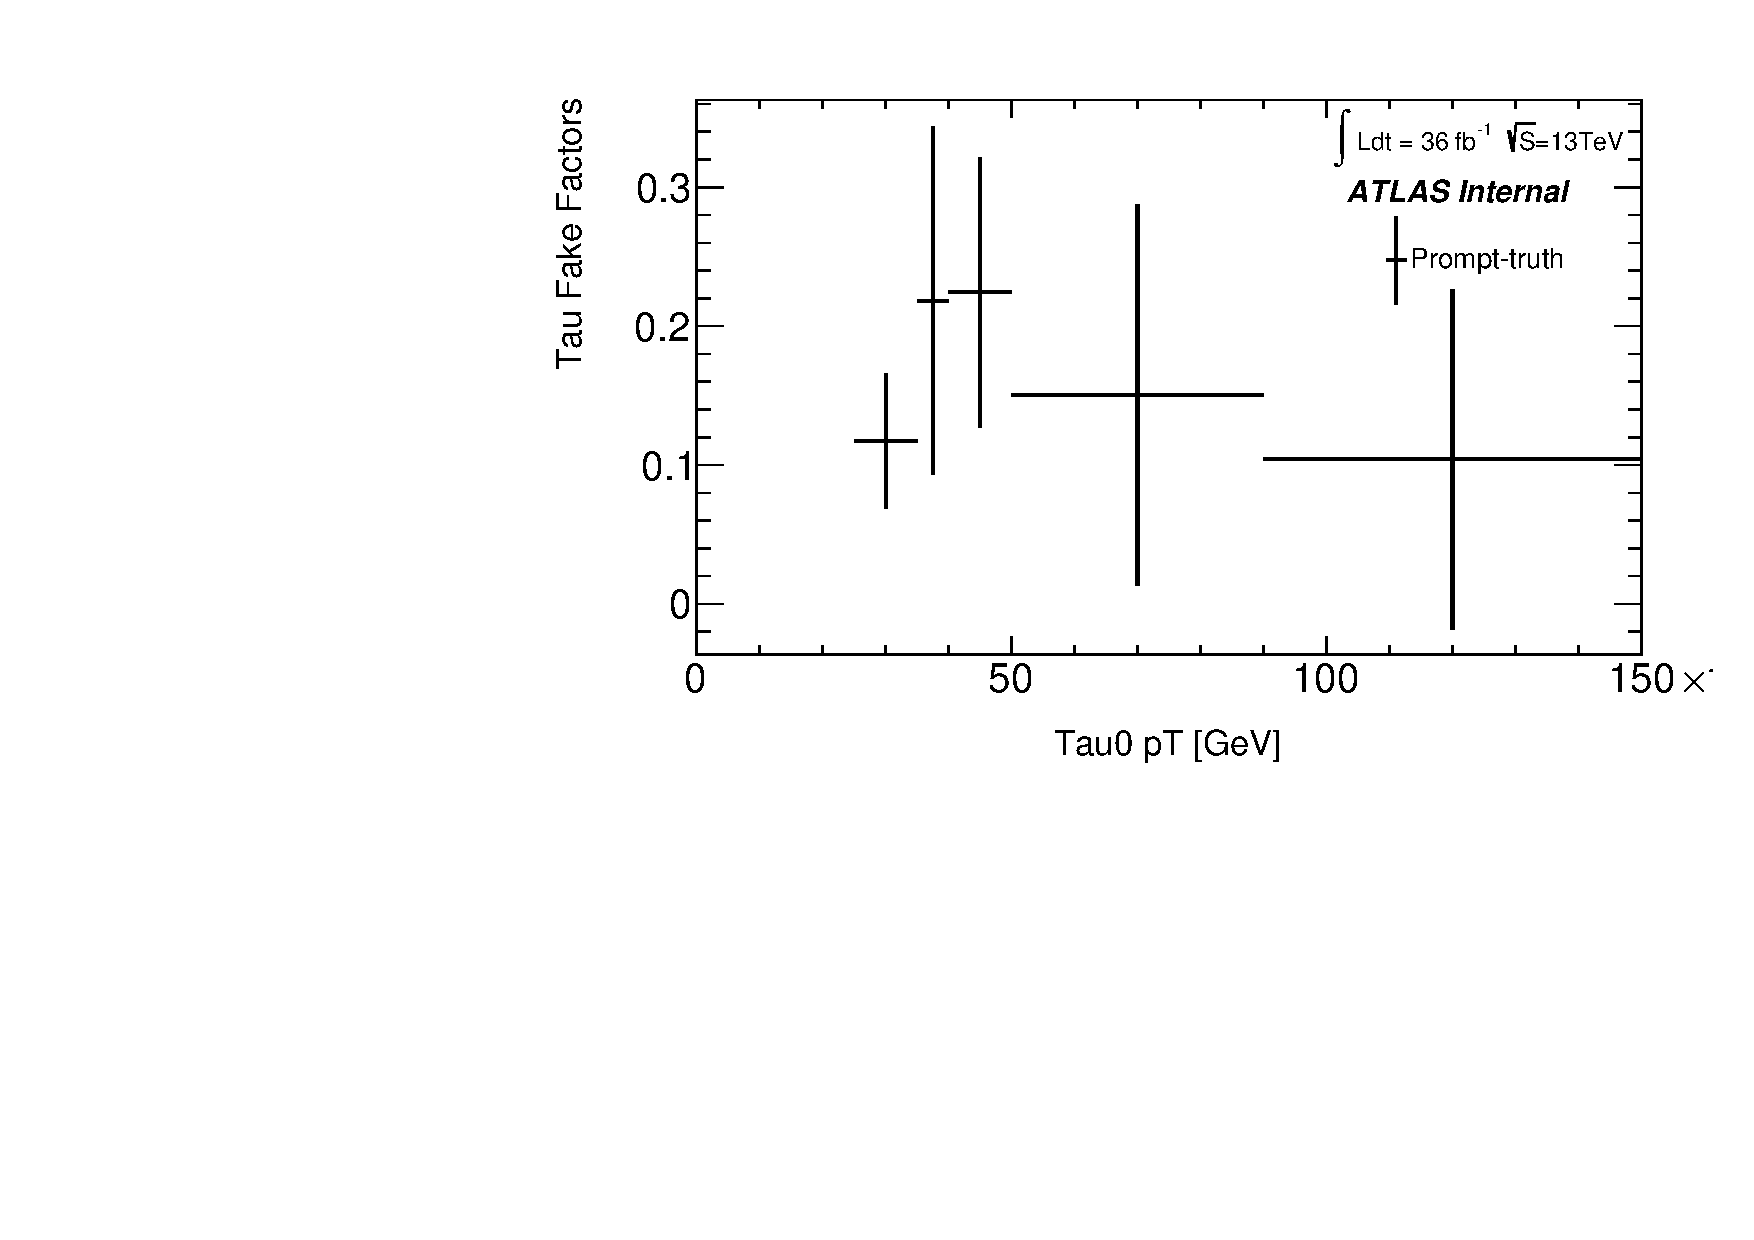
\includegraphics[width=0.95\linewidth]{figures/FakesEstimate_data_pp8_nonallhad_new_scaledHists/FF_Faketau_Prompt-truth.pdf}
  	\caption{$p_T$-parametrized fake factors}
  	\label{fig:sub1}
	\end{subfigure}%
	\begin{subfigure}{.5\textwidth}
	\centering
	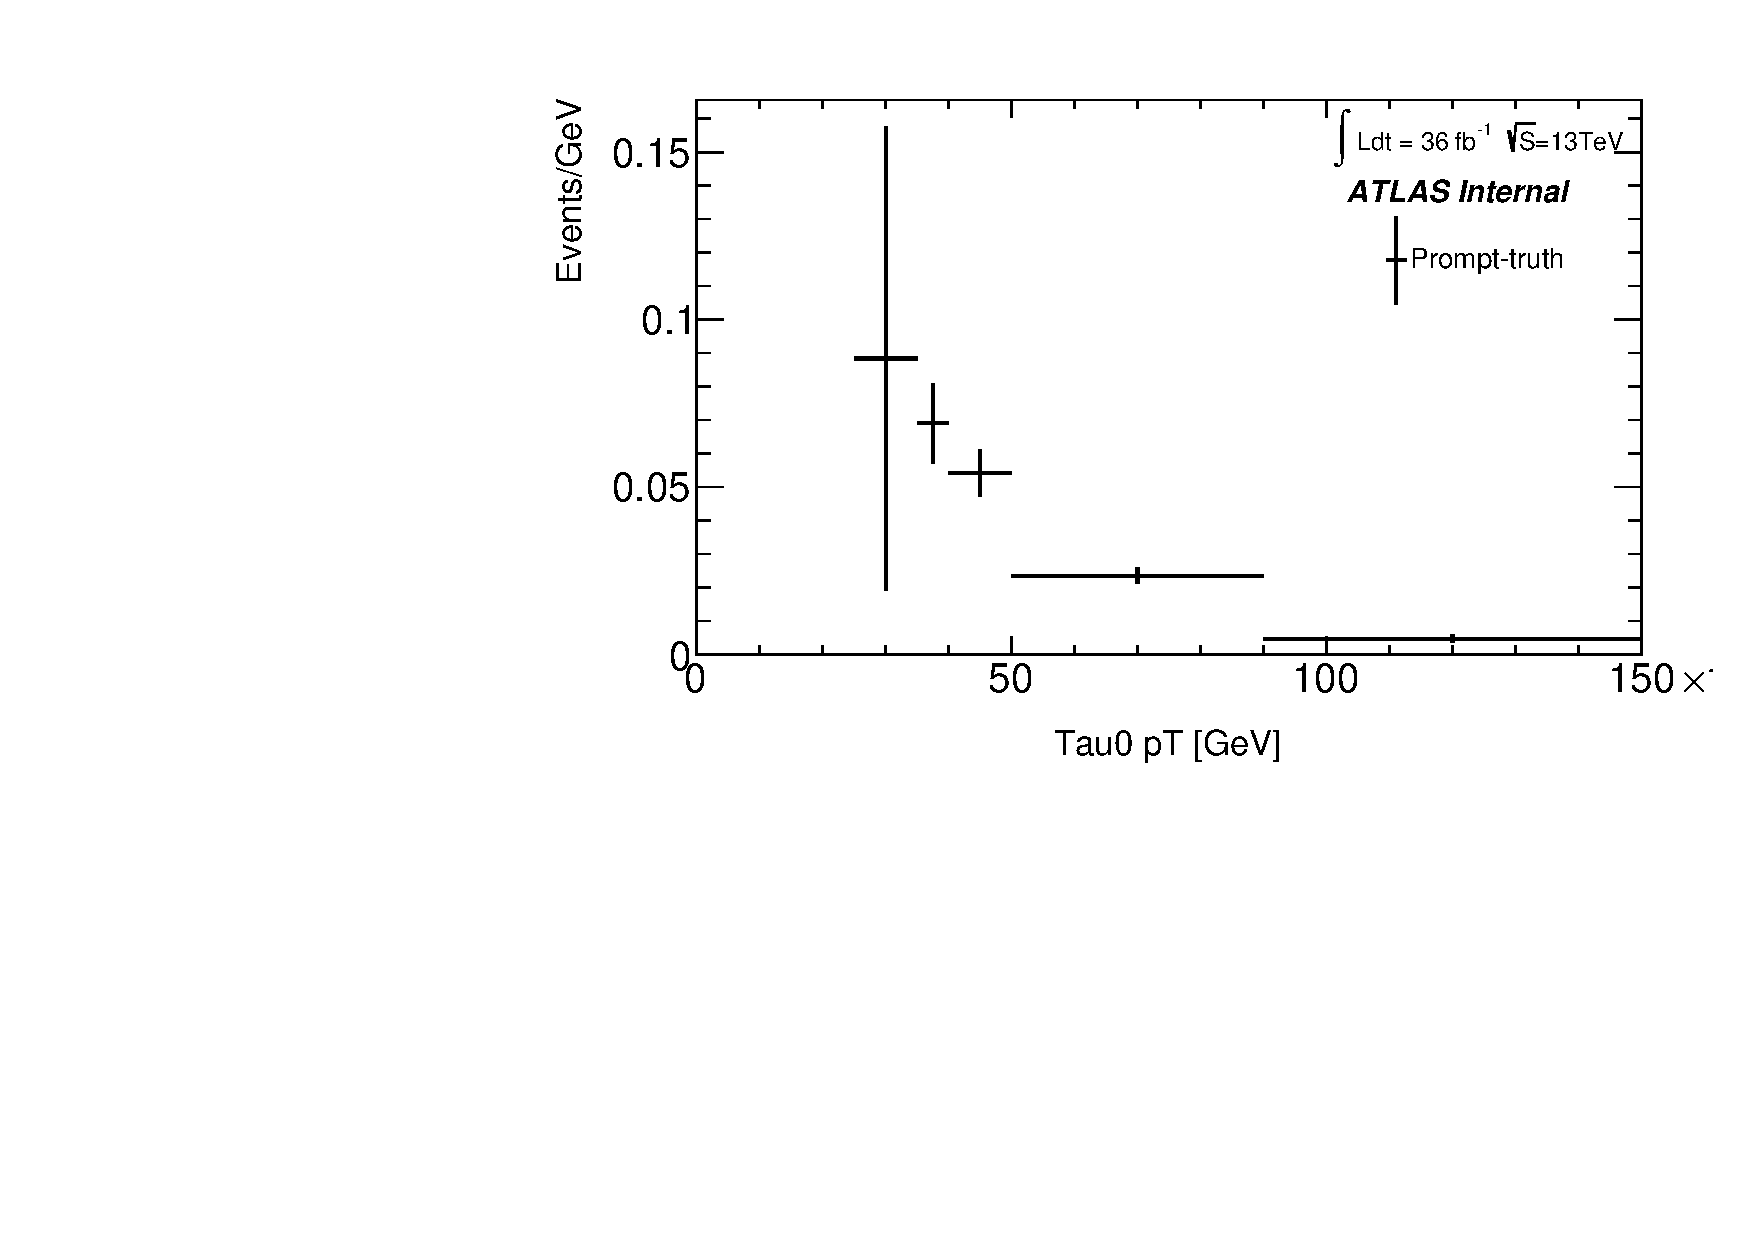
\includegraphics[width=0.95\linewidth]{figures/FakesEstimate_data_pp8_nonallhad_new_scaledHists/hist_Extrapolation_Prompt-truth.pdf}
	\caption{Extrapolation sideband region $p_T$ spectrum}
	\end{subfigure}
	\caption{Fake factors and extrapolation sideband region, (Prompt MC - truth)}
	\end{figure}
	
	\begin{figure}[H]
	\centering
	\begin{subfigure}{.5\textwidth}
	\centering
	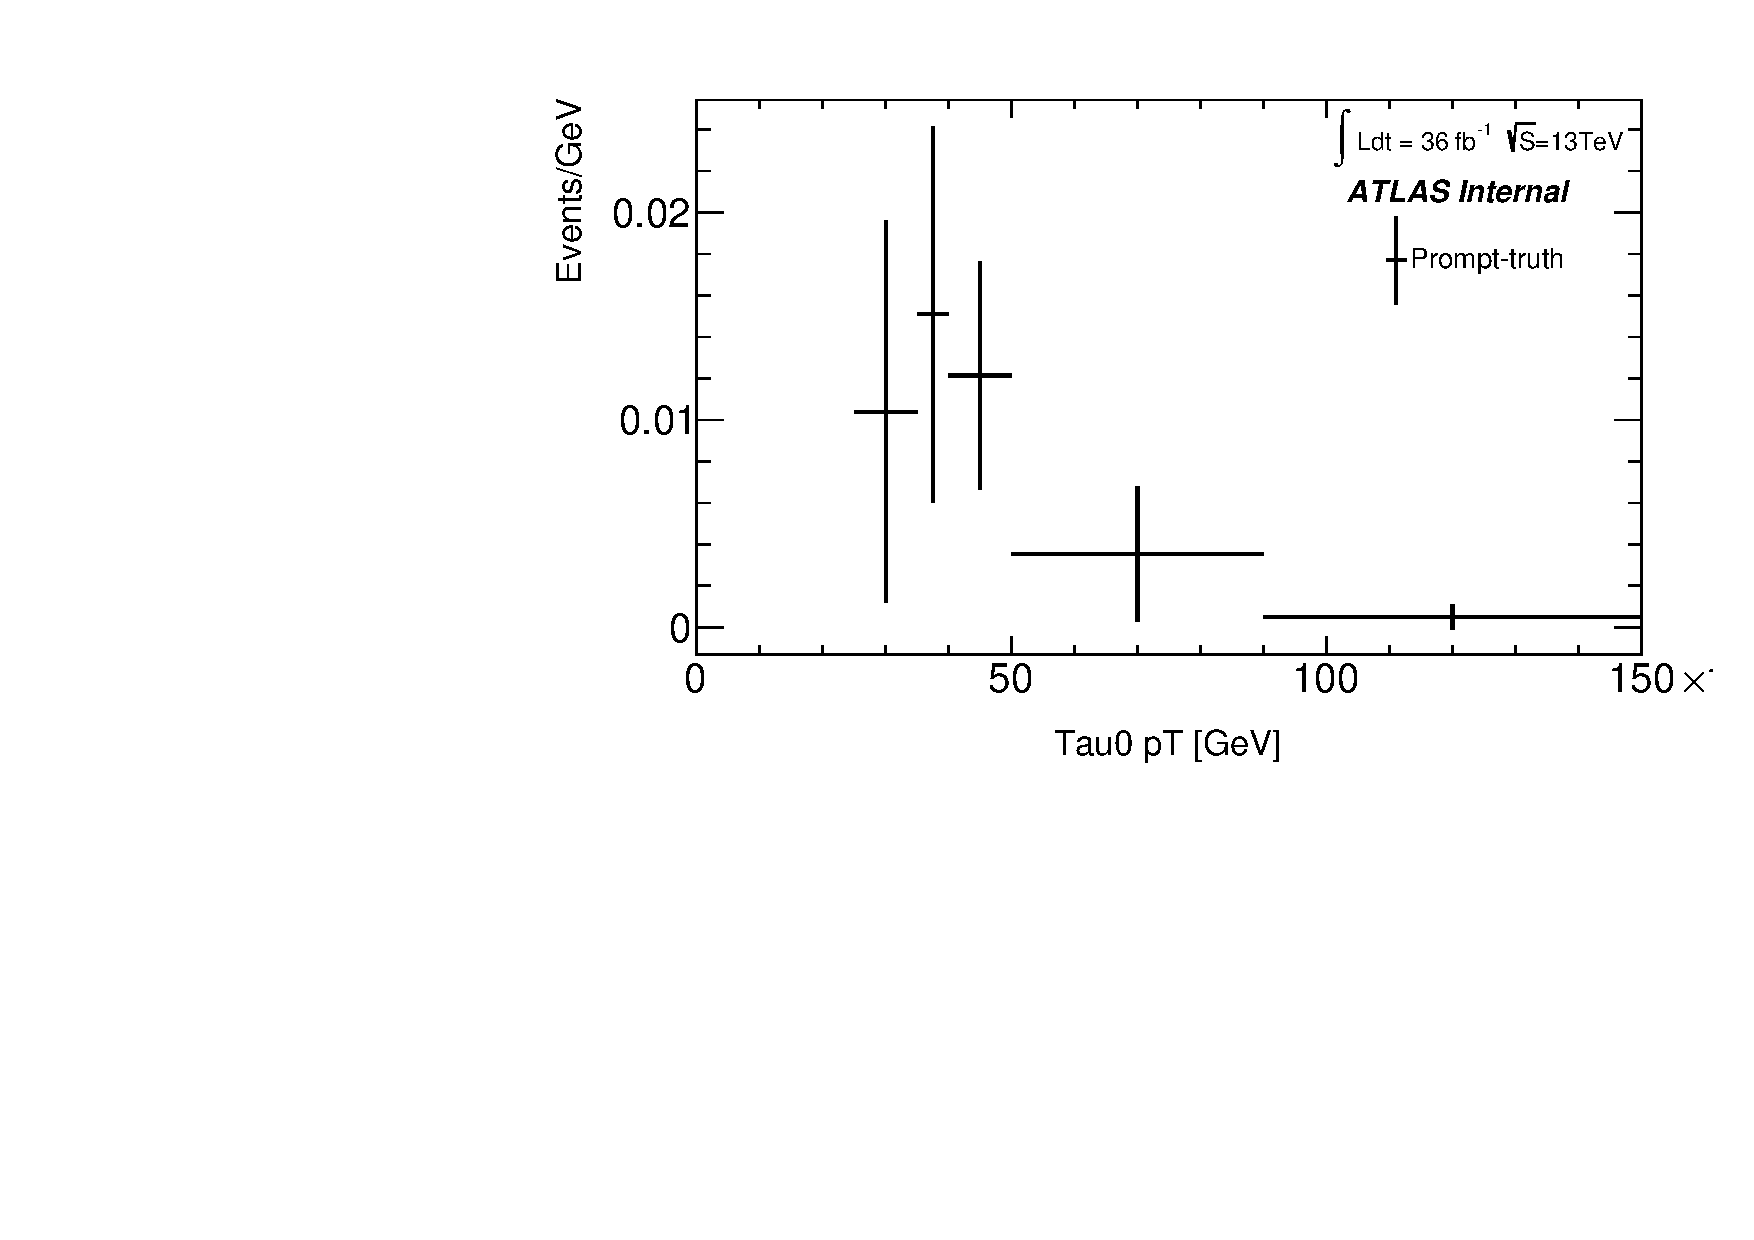
\includegraphics[width=0.95\linewidth]{figures/FakesEstimate_data_pp8_nonallhad_new_scaledHists/hist_FakeEstimate_Prompt-truth.pdf}
  	\caption{Fake estimate in $p_T$ bins}
  	\label{fig:sub1}
	\end{subfigure}%
	\begin{subfigure}{.5\textwidth}
	\centering
	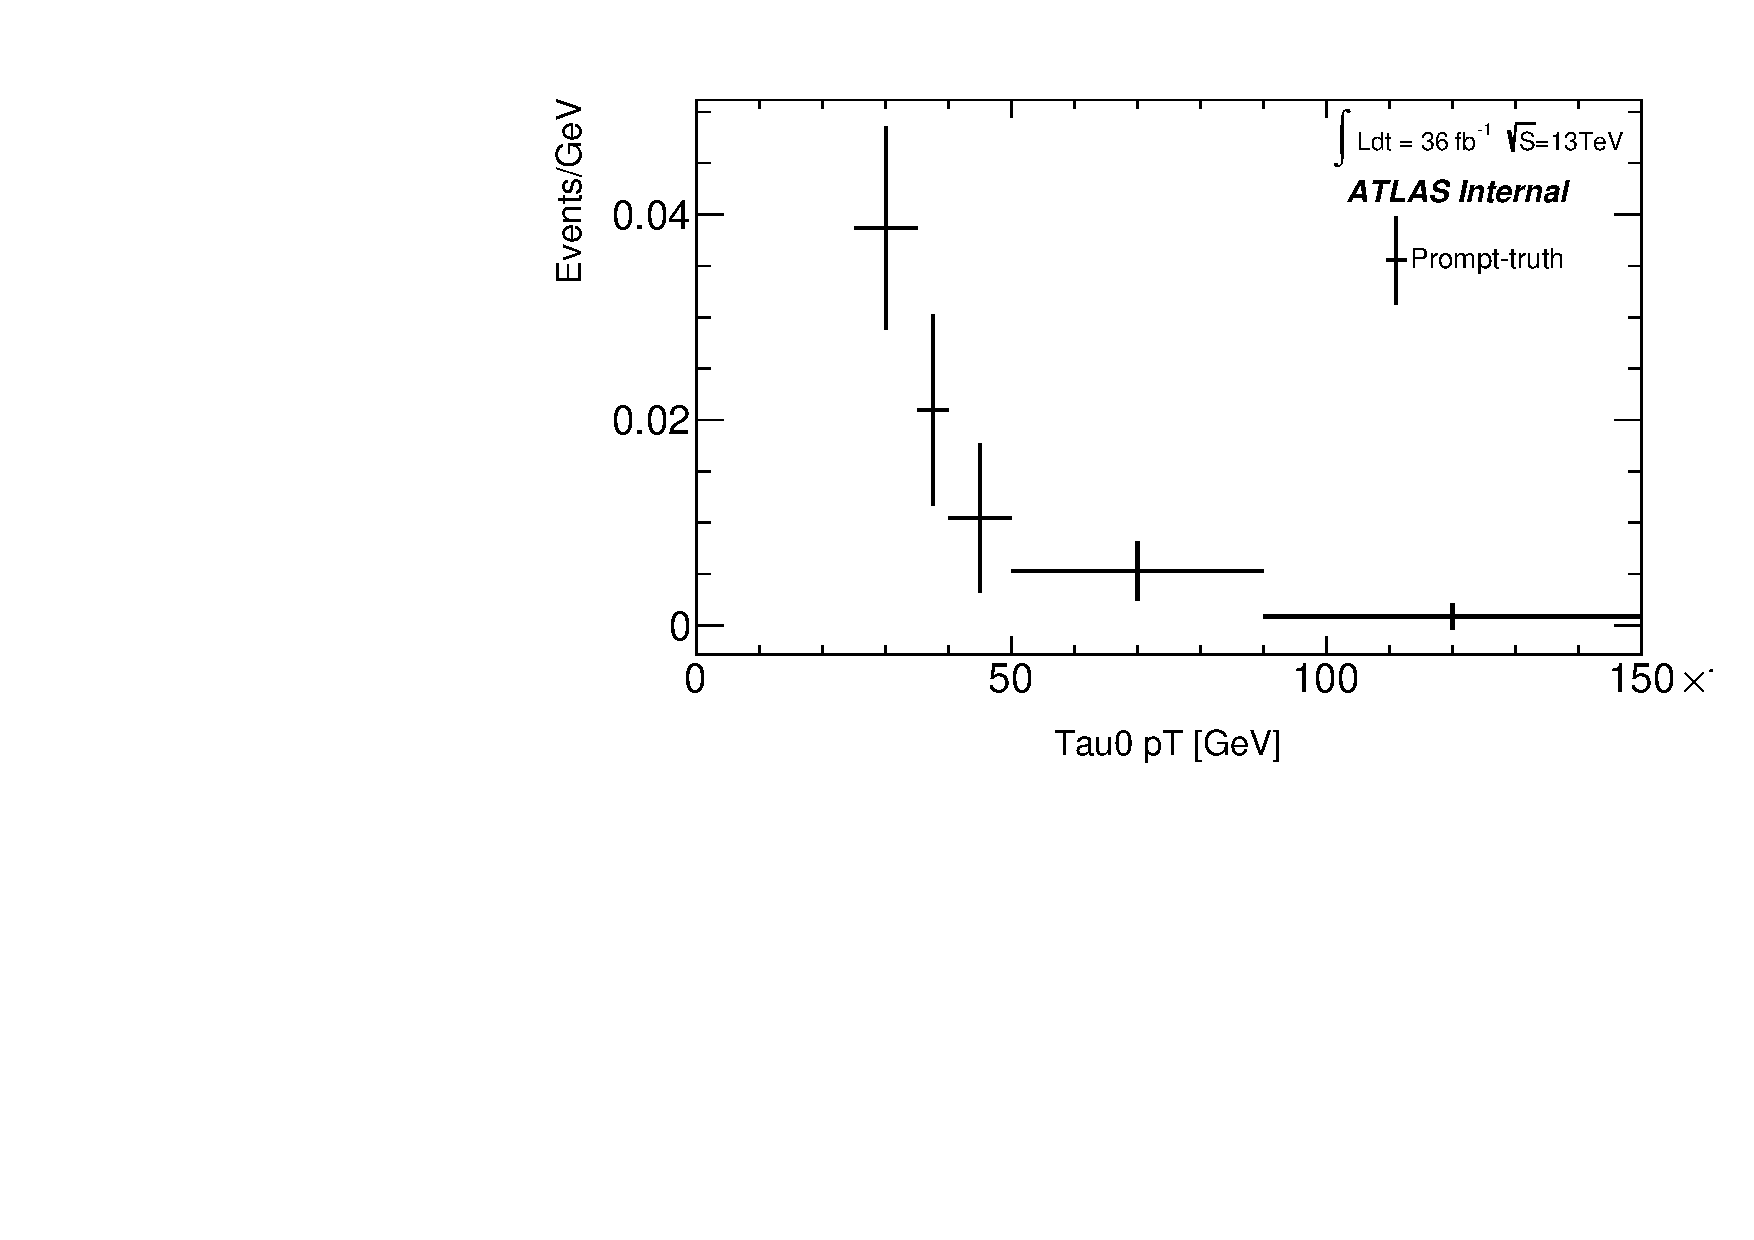
\includegraphics[width=0.95\linewidth]{figures/FakesEstimate_data_pp8_nonallhad_new_scaledHists/hist_SRMC_Prompt-truth.pdf}
	\caption{MC SR yield in $p_T$ bins}
	\end{subfigure}
	\caption{$p_T$ spectra for fake estimate and MC yield, (Prompt MC - truth)}
	\end{figure}

	\begin{figure}[H]
		\centering
		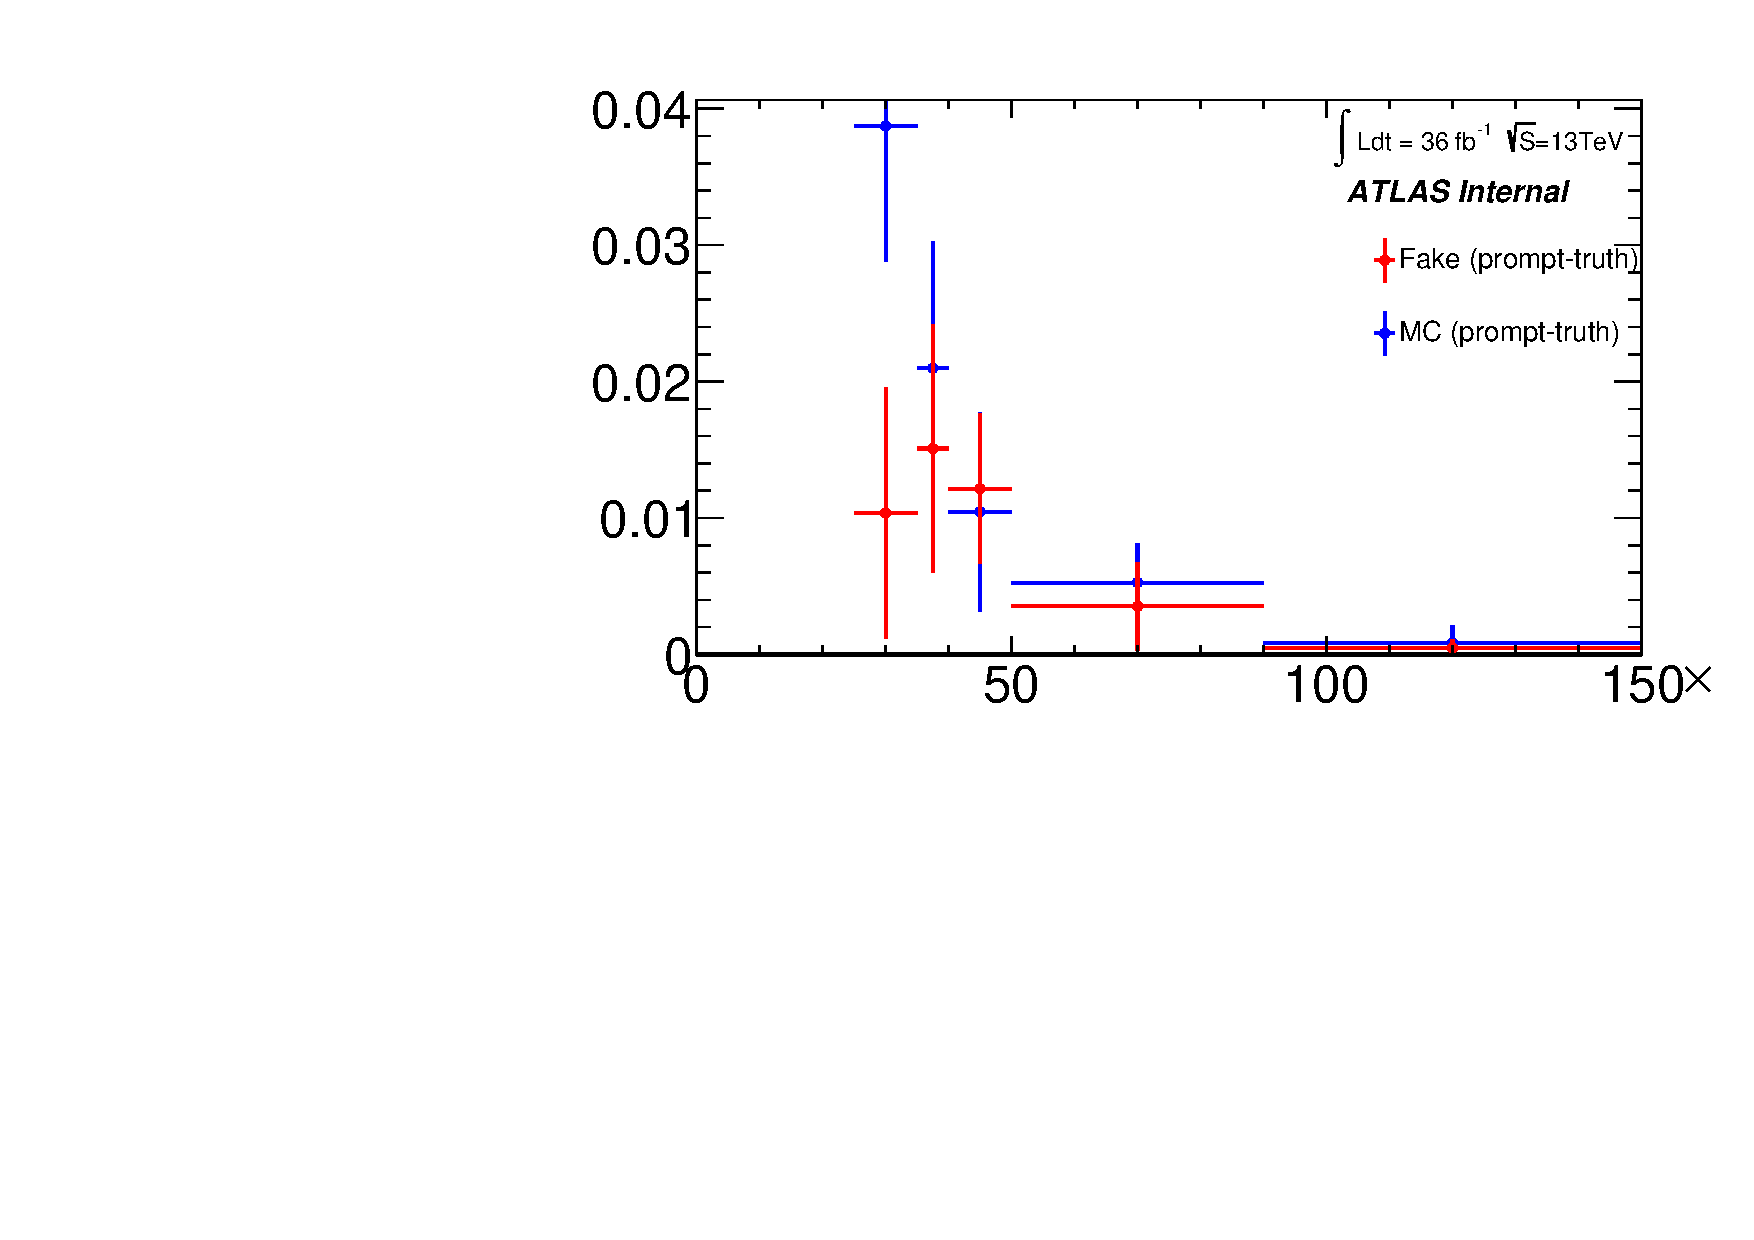
\includegraphics[width=0.7\linewidth]{figures/FakesEstimate_data_pp8_nonallhad_new_scaledHists/Overlay_FF_tau_pt_prompt-truth.pdf}
		\caption{Overlaid fake estimate and MC prediction (Prompt MC - truth)}
	\end{figure}		
			
			
	\subsection{$\tau_{had}$ Truth origin studies} 	
			
	\begin{figure}[H]
		\begin{subfigure}[b]{.5\textwidth}
			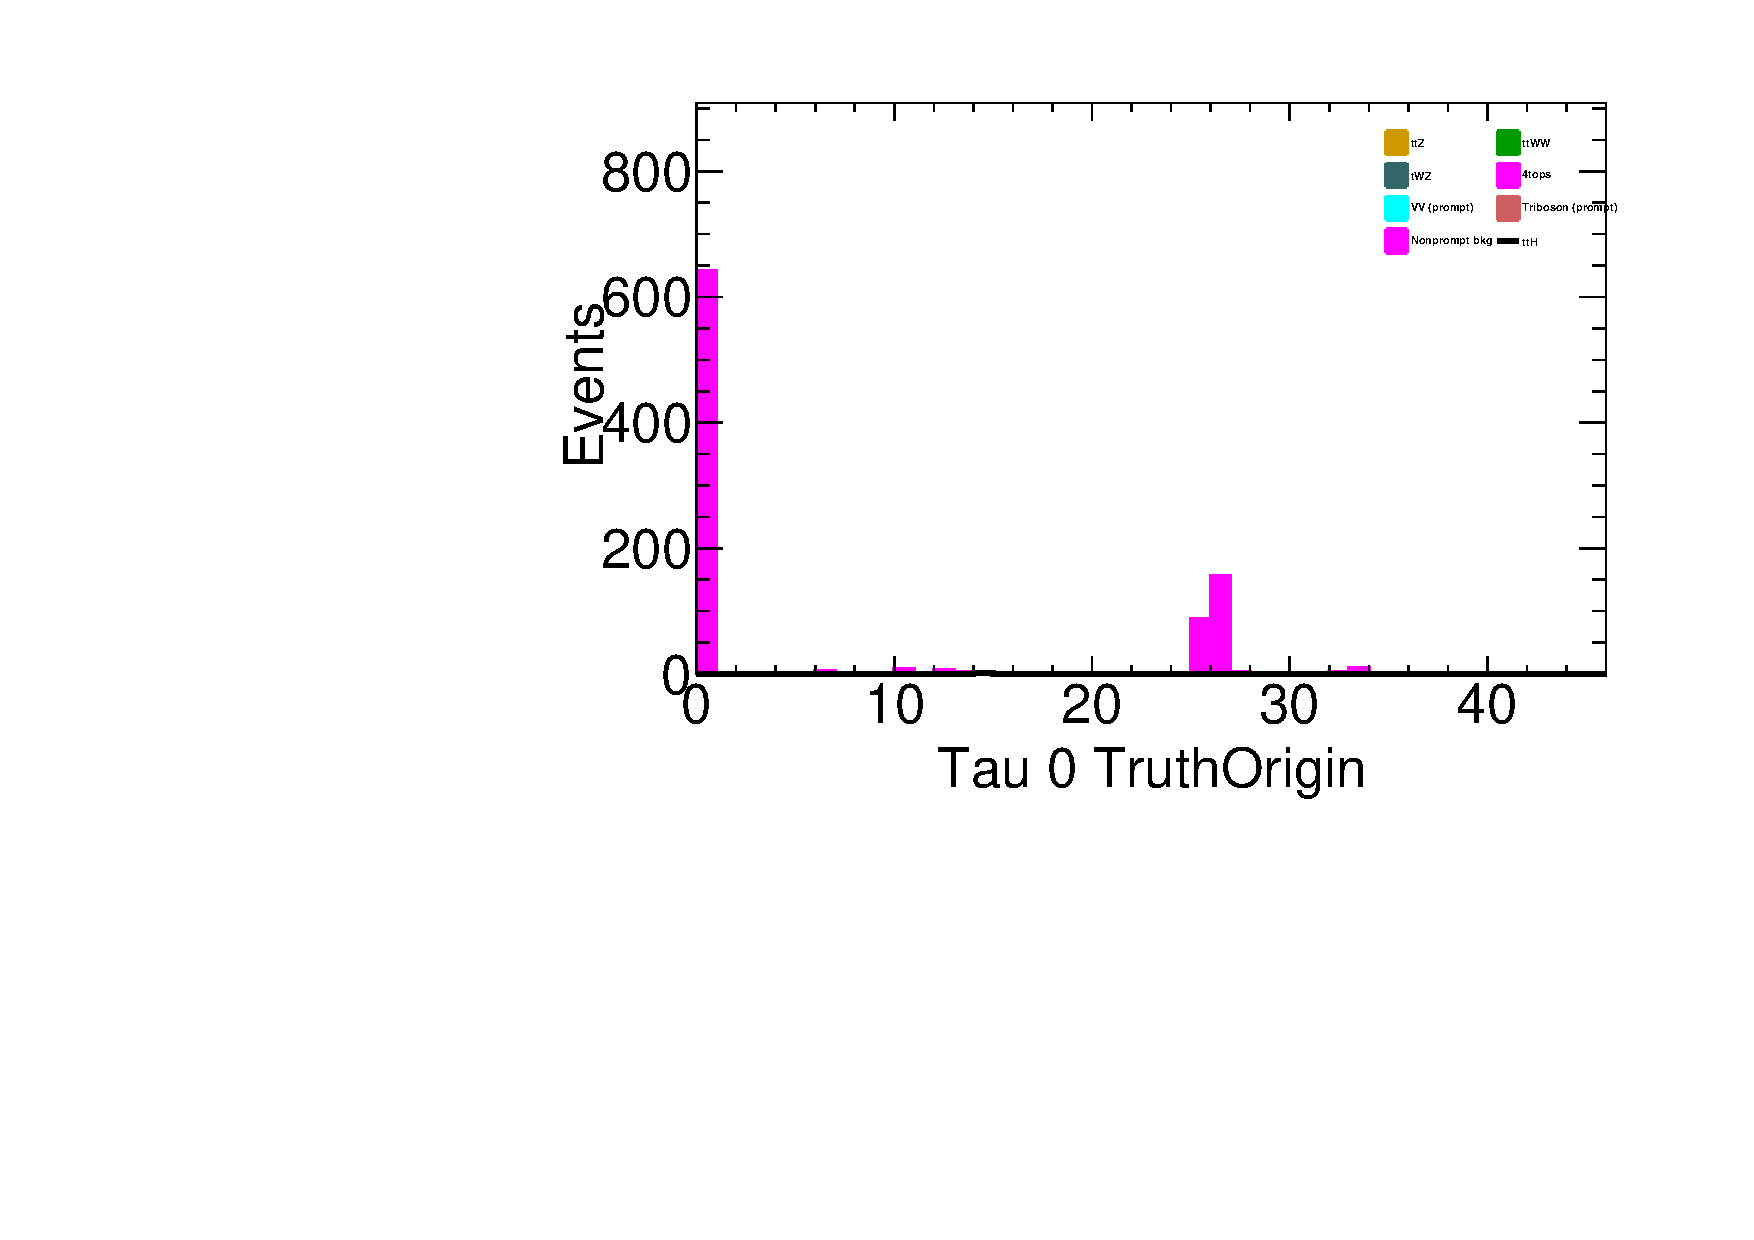
\includegraphics[width=0.82\linewidth]{figures/Plots_MC_April10_pp8-new_PromptPlots/2lOStau_CR_TightLepMVA_TauMedium_eq2j_ge1b_Tau0TruthOrigin.pdf}
  			\caption{Numerator region}
		\end{subfigure}
		\hfill
		\begin{subfigure}[b]{.5\textwidth}
			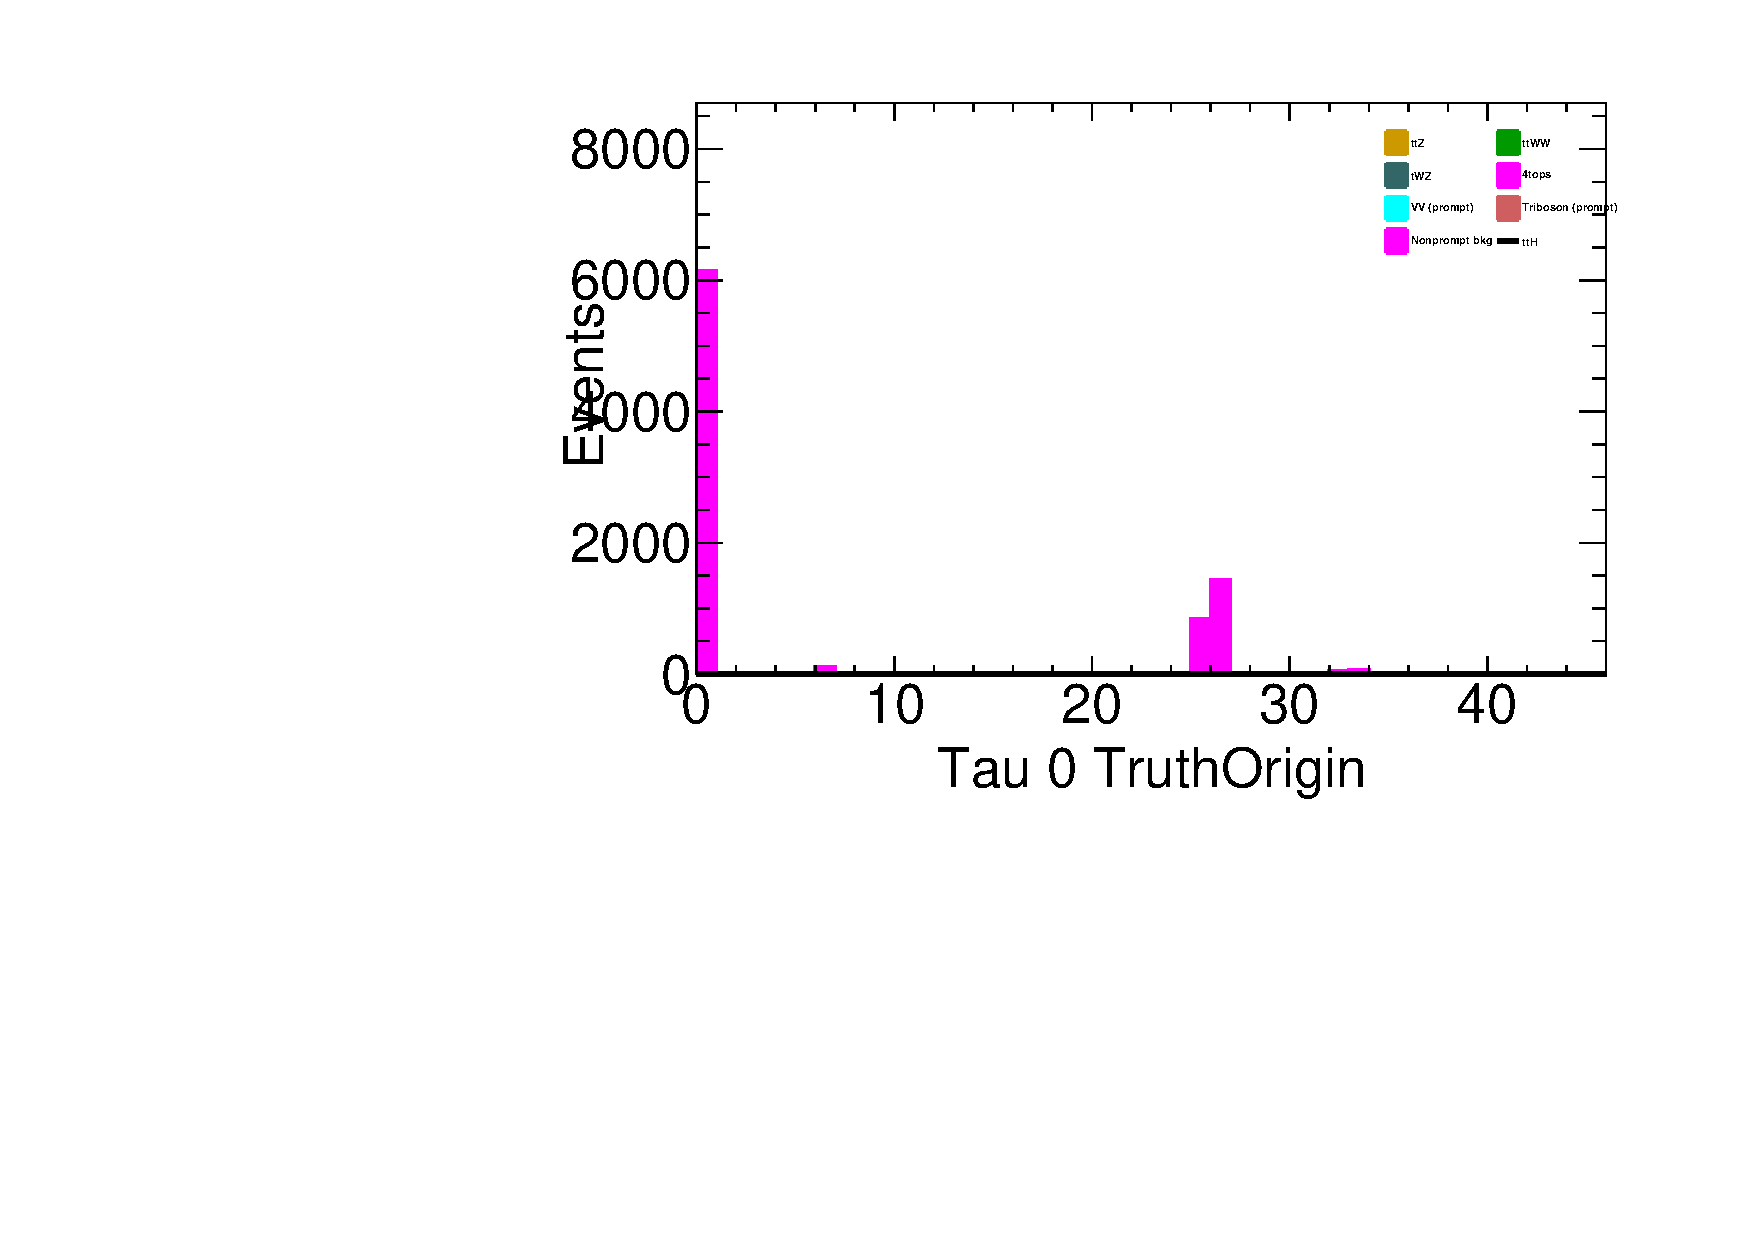
\includegraphics[width=0.82\linewidth]{figures/Plots_MC_April10_pp8-new_PromptPlots/2lOStau_CR_TightLepMVA_TauVeryLooseNotMedium_eq2j_ge1b_Tau0TruthOrigin.pdf}
			\caption{Denominator ($\cancel{\tau}$) region }
		\end{subfigure}%
		\vskip\baselineskip
		\begin{subfigure}[b]{.5\textwidth}
			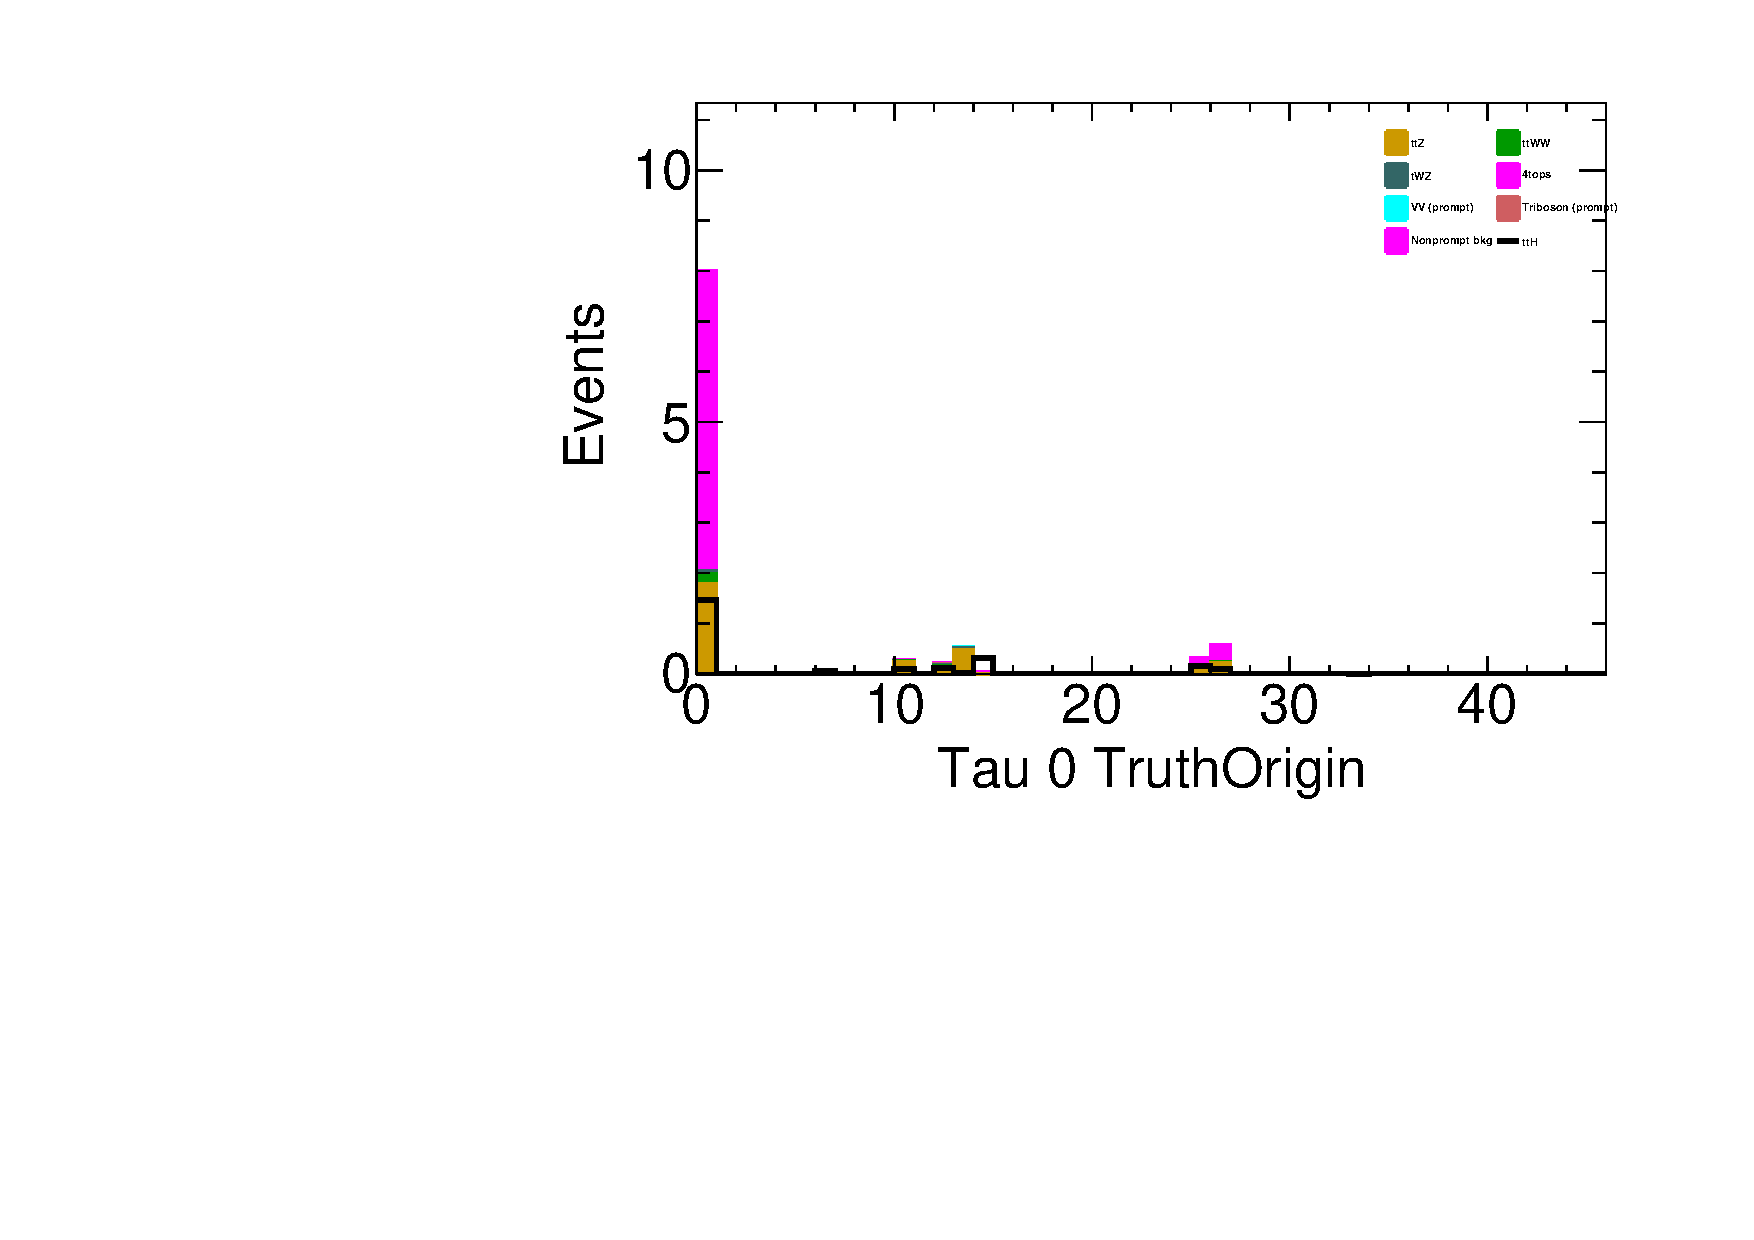
\includegraphics[width=0.82\linewidth]{figures/Plots_MC_April10_pp8-new_PromptPlots/3ltau_SR_TightLepMVA_TauVeryLooseNotMedium_Tau0TruthOrigin.pdf}
			\caption{Extrapolation region}
		\end{subfigure}
		\quad
		\begin{subfigure}[b]{.5\textwidth}
			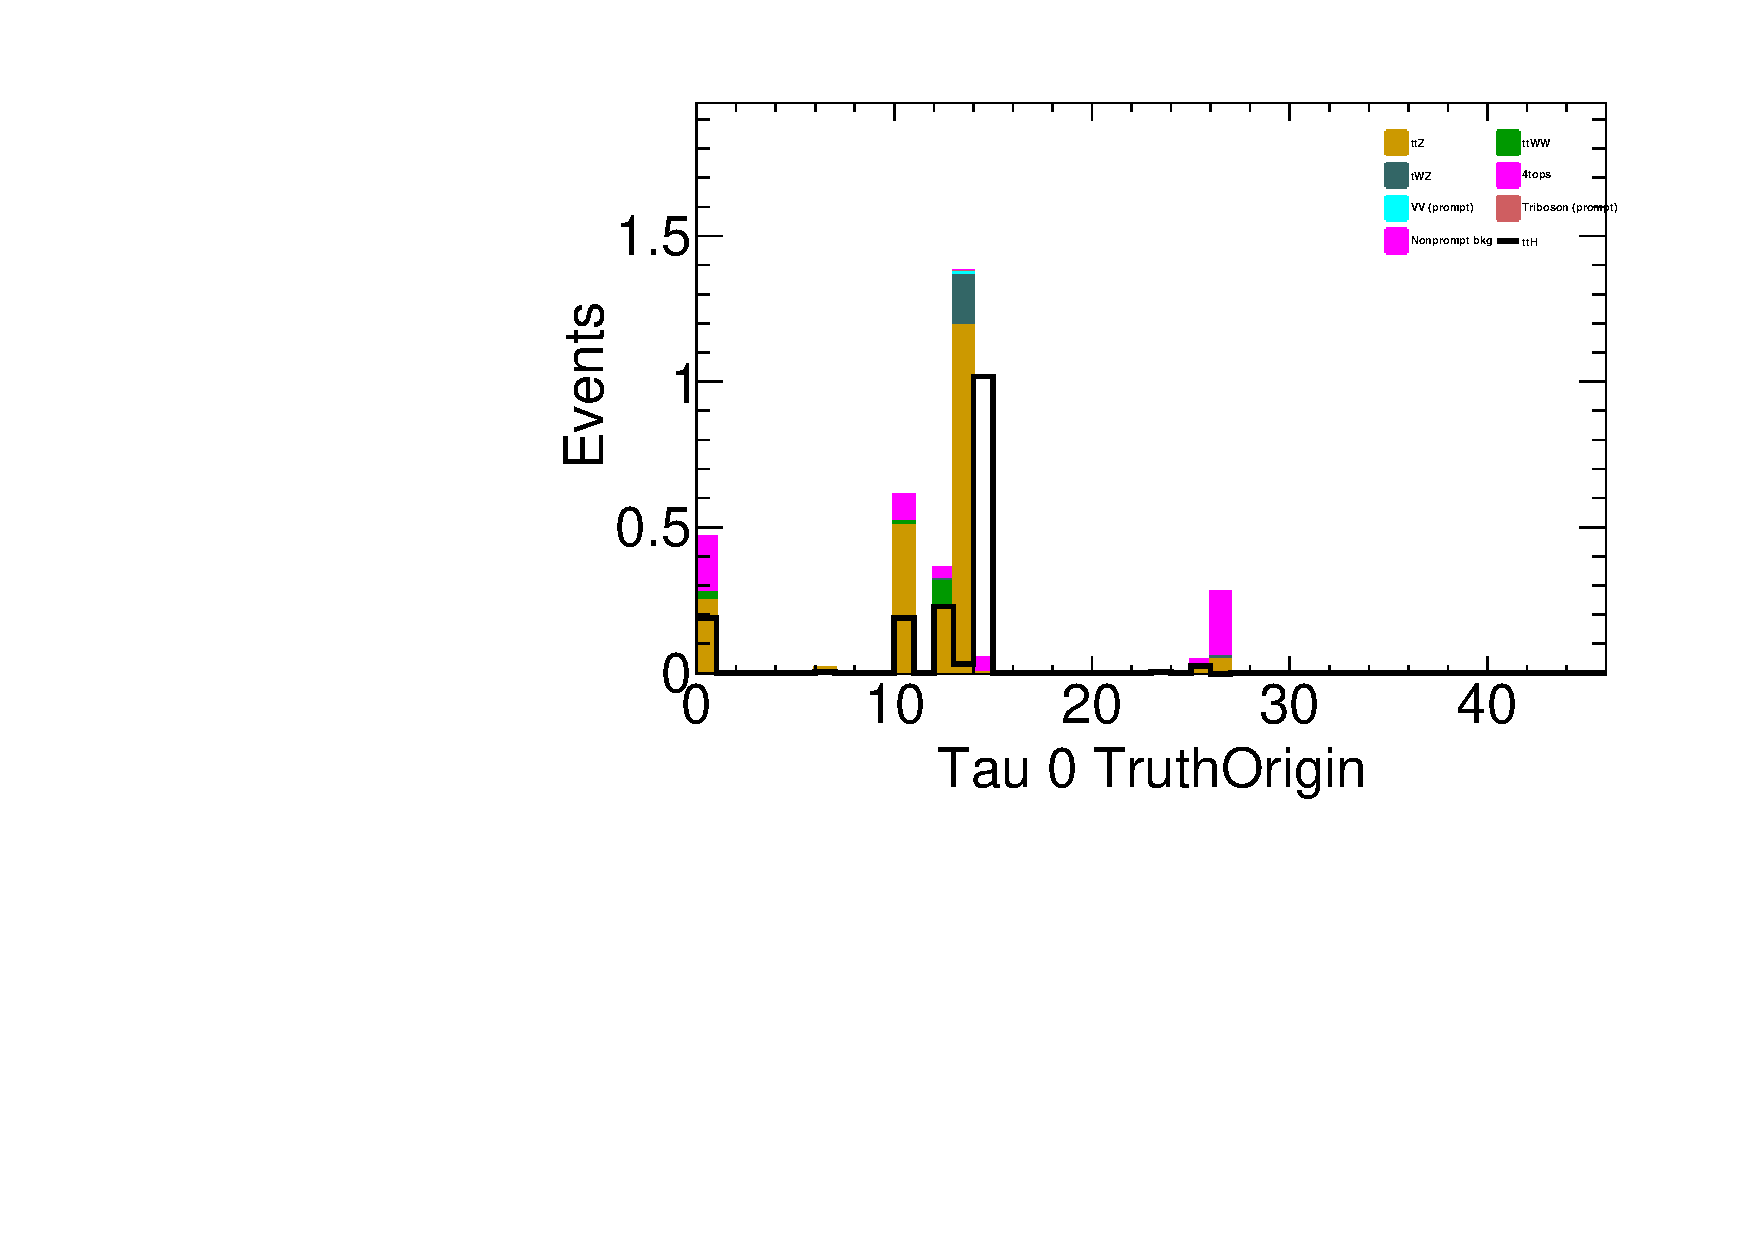
\includegraphics[width=0.82\linewidth]{figures/Plots_MC_April10_pp8-new_PromptPlots/3ltau_SR_TightLepMVA_TauMedium_Tau0TruthOrigin.pdf}
			\caption{Signal region}
		\end{subfigure}
		\caption{Truth origin of $\tau_{had}$ in fake-estimate control regions and signal region}
	\end{figure}
			
	\begin{figure}[H]
		\centering
		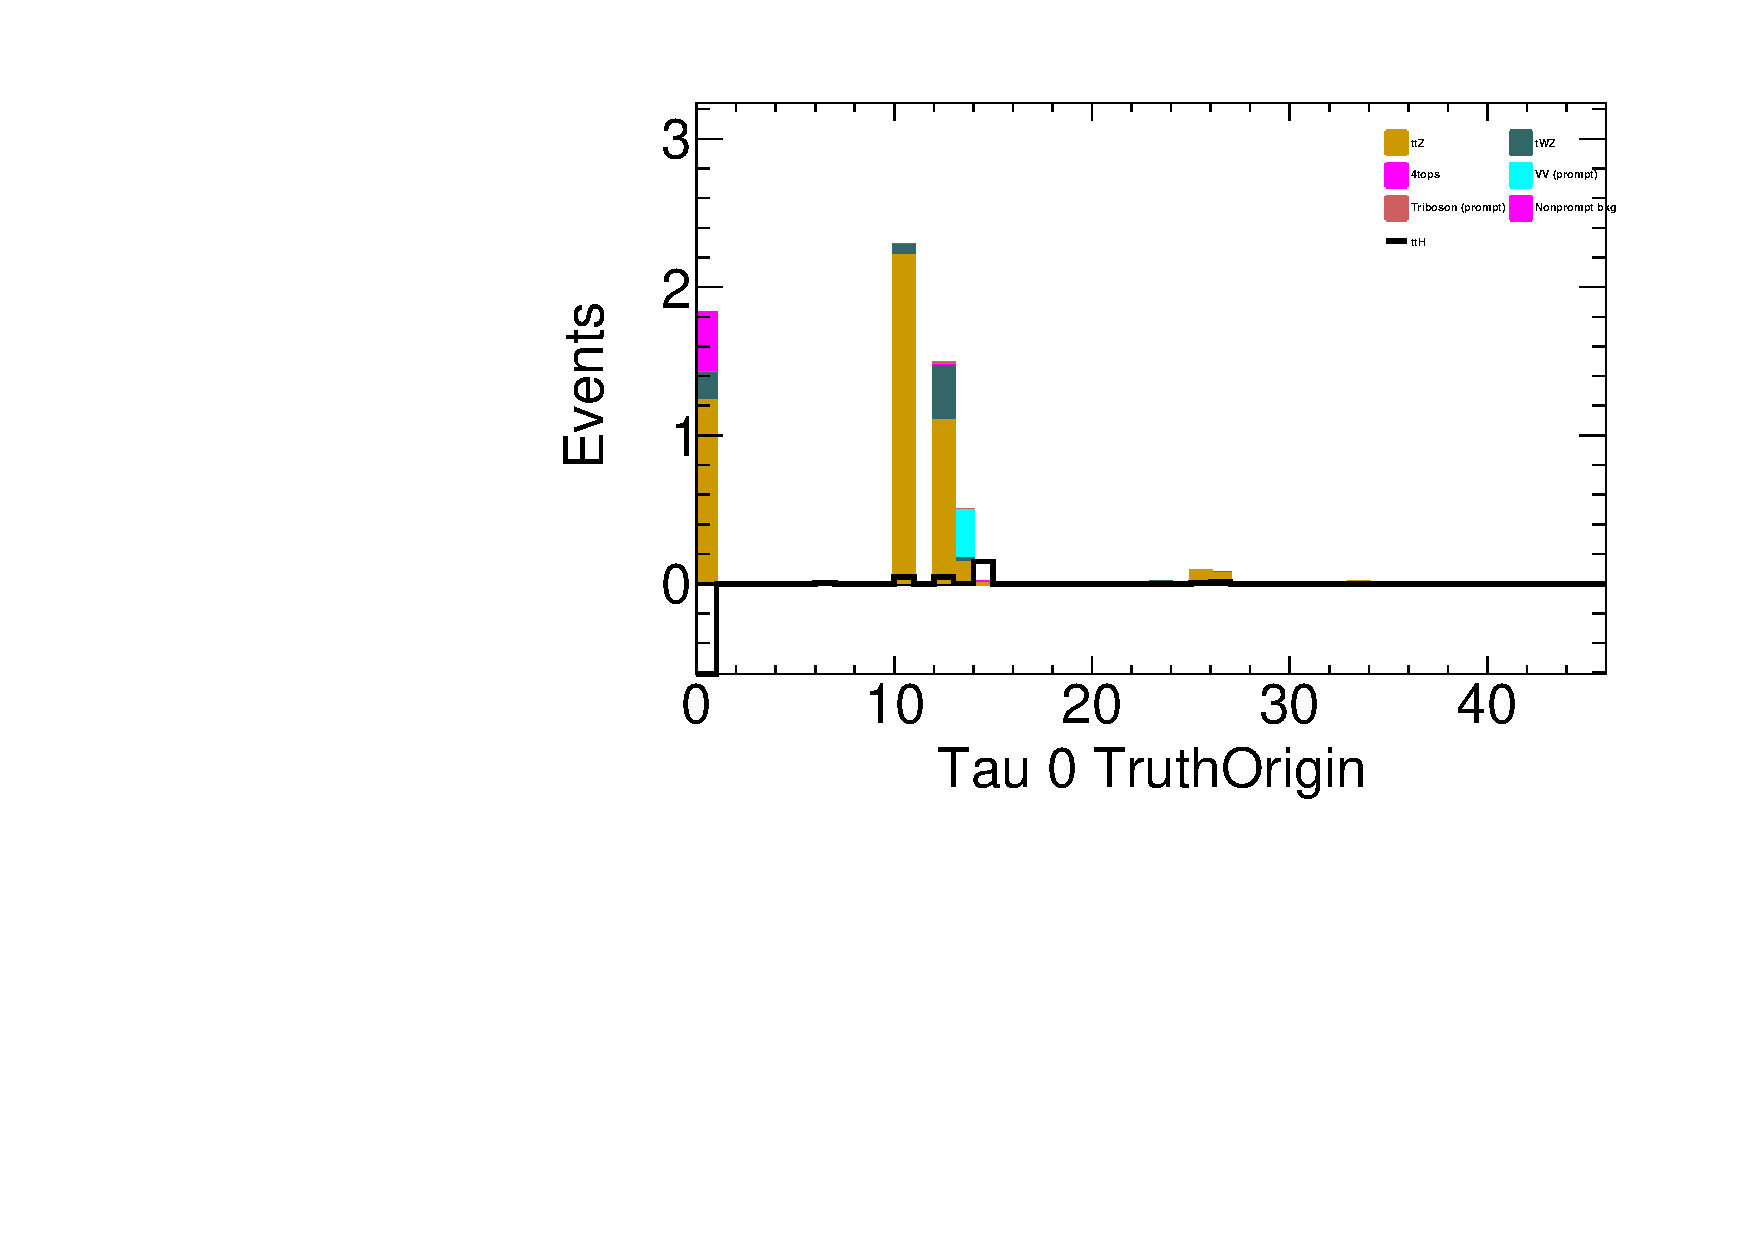
\includegraphics[width=0.65\linewidth]{figures/Plots_MC_April10_pp8-new_PromptPlots/3ltau_ttZ_CR_TightLepMVA_TauMedium_Tau0TruthOrigin.pdf}
		\caption{Truth origin of $\tau_{had}$ in $t\bar{t}Z$ control region (signal region selection + selecting events with 1 pair of OS-SF leptons within the Z-mass window}
	\end{figure}		
			
		

	\begin{table}[htp]
		\caption{Monte Carlo samples \& categorization}
		\begin{center}
			\begin{tabular}{|l|p{10cm}|}
			\hline
			ttH & \textcolor{blue}{343365} \textcolor{blue}{343366} \textcolor{blue}{343367} \\
			\hline
			Prompt bkg & ttZ, ttWW, tWZ, 4top, VH, diboson (4l) and triboson (4l): \textcolor{blue}{342284} \textcolor{blue}{342285} \textcolor{blue}{361063} \textcolor{blue}{361072} \textcolor{blue}{361073} \textcolor{blue}{361621} \textcolor{blue}{361623} \textcolor{blue}{361625} \textcolor{blue}{361626} \textcolor{blue}{410080} \textcolor{blue}{410081} \textcolor{blue}{410156} \textcolor{blue}{410157} \textcolor{blue}{410215} \textcolor{blue}{410218} \textcolor{blue}{410219} \textcolor{blue}{410220} \\
			\hline
			Nonprompt bkg &  tZ, ttW, 3top, single top, Z+jets, W+jets, diboson (non-4l), triboson (non-4l), tHbj, ttbar: \textcolor{blue}{304014} \textcolor{blue}{341998} \textcolor{blue}{342001} \textcolor{blue}{342004} \textcolor{blue}{343267} \textcolor{blue}{343270} \textcolor{blue}{343273} \textcolor{blue}{361064} \textcolor{blue}{361065} \textcolor{blue}{361066} \textcolor{blue}{361067} \textcolor{blue}{361068} \textcolor{blue}{361069} \textcolor{blue}{361070} \textcolor{blue}{361071} \textcolor{blue}{361077} \textcolor{blue}{361091} \textcolor{blue}{361092} \textcolor{blue}{361093} \textcolor{blue}{361094} \textcolor{blue}{361095} \textcolor{blue}{361096} \textcolor{blue}{361097} \textcolor{blue}{361620} \textcolor{blue}{361622} \textcolor{blue}{361624} \textcolor{blue}{361627} \textcolor{blue}{364100} \textcolor{blue}{364101} \textcolor{blue}{364102} \textcolor{blue}{364103} \textcolor{blue}{364104} \textcolor{blue}{364105} \textcolor{blue}{364106} \textcolor{blue}{364107} \textcolor{blue}{364108} \textcolor{blue}{364109} \textcolor{blue}{364110} \textcolor{blue}{364111} \textcolor{blue}{364112} \textcolor{blue}{364113} \textcolor{blue}{364114} \textcolor{blue}{364115} \textcolor{blue}{364116} \textcolor{blue}{364117} \textcolor{blue}{364118} \textcolor{blue}{364119} \textcolor{blue}{364120} \textcolor{blue}{364121} \textcolor{blue}{364122} \textcolor{blue}{364123} \textcolor{blue}{364124} \textcolor{blue}{364125} \textcolor{blue}{364126} \textcolor{blue}{364127} \textcolor{blue}{364128} \textcolor{blue}{364129} \textcolor{blue}{364130} \textcolor{blue}{364131} \textcolor{blue}{364132} \textcolor{blue}{364133} \textcolor{blue}{364134} \textcolor{blue}{364135} \textcolor{blue}{364136} \textcolor{blue}{364137} \textcolor{blue}{364138} \textcolor{blue}{364139} \textcolor{blue}{364140} \textcolor{blue}{364141} \textcolor{blue}{364156} \textcolor{blue}{364157} \textcolor{blue}{364158} \textcolor{blue}{364159} \textcolor{blue}{364160} \textcolor{blue}{364161} \textcolor{blue}{364162} \textcolor{blue}{364163} \textcolor{blue}{364164} \textcolor{blue}{364165} \textcolor{blue}{364166} \textcolor{blue}{364167} \textcolor{blue}{364168} \textcolor{blue}{364169} \textcolor{blue}{364170} \textcolor{blue}{364171} \textcolor{blue}{364172} \textcolor{blue}{364173} \textcolor{blue}{364174} \textcolor{blue}{364175} \textcolor{blue}{364176} \textcolor{blue}{364177} \textcolor{blue}{364178} \textcolor{blue}{364179} \textcolor{blue}{364180} \textcolor{blue}{364181} \textcolor{blue}{364182} \textcolor{blue}{364183} \textcolor{blue}{364184} \textcolor{blue}{364185} \textcolor{blue}{364186} \textcolor{blue}{364187} \textcolor{blue}{364188} \textcolor{blue}{364189} \textcolor{blue}{364190} \textcolor{blue}{364191} \textcolor{blue}{364192} \textcolor{blue}{364193} \textcolor{blue}{364194} \textcolor{blue}{364195} \textcolor{blue}{364196} \textcolor{blue}{364197} \textcolor{blue}{364198} \textcolor{blue}{364199} \textcolor{blue}{364200} \textcolor{blue}{364201} \textcolor{blue}{364202} \textcolor{blue}{364203} \textcolor{blue}{364204} \textcolor{blue}{364205} \textcolor{blue}{364206} \textcolor{blue}{364207} \textcolor{blue}{364208} \textcolor{blue}{364209} \textcolor{blue}{364210} \textcolor{blue}{364211} \textcolor{blue}{364212} \textcolor{blue}{364213} \textcolor{blue}{364214} \textcolor{blue}{364215} \textcolor{blue}{410011} \textcolor{blue}{410012} \textcolor{blue}{410015} \textcolor{blue}{410016} \textcolor{blue}{410025} \textcolor{blue}{410026} \textcolor{blue}{410049} \textcolor{blue}{410155} \textcolor{blue}{410501}\\
			\hline
			\end{tabular}
		\end{center}
		\label{mc_samples}
	\end{table}





	\clearpage
	\subsection{Estimate with non-prompt MC} 
	Here there is no subtraction performed and the estimate and closure test is done on the non-prompt MC only. 
	\begin{equation}
		FF(p_T)_{MC} = \frac{N_\tau (p_T)^{\text{Non-prompt MC}}}{N_{\cancel{\tau}} (p_T)^{\text{Non-prompt MC}}}
	\end{equation}

	
	\begin{table}[htp]
	\caption{Extrapolation and closure test, (Non-prompt MC)}
	\begin{center}
	\begin{tabular}{|c|c|c|c|c|}
	\hline
	$t\bar{t}$ sample 	& Integrated fake estimate	& SR MC		& Raw		& 	 Closure \\
	\hline
	PP8 non-all hadronic			& 	$0.590\pm0.146$ 		& $0.704\pm0.405$ 		& 238	&  $19\pm75$\% \\
	PP8 non-all hadronic, high stats	& 	$0.661\pm0.130$ 		& $0.510\pm0.213$ 		& 238	&  $-23\pm36$\% \\
	PP8 dilepton 					& 	$0.454\pm0.105$ 		& $0.532\pm0.234$ 		& 238	&  $17\pm58$\% \\
	PP8 dilepton, high stats			& 	$0.530\pm0.089$ 		& $0.706\pm0.241$ 		& 240	&  $33\pm50$\% \\
	\hline
	\end{tabular}
	\end{center}
	\label{default}
	\end{table}%
		
	Figures are produced using the non-all hadronic high-stats sample. 
	
	\begin{figure}[H]
	\centering
	\begin{subfigure}{.5\textwidth}
	\centering
	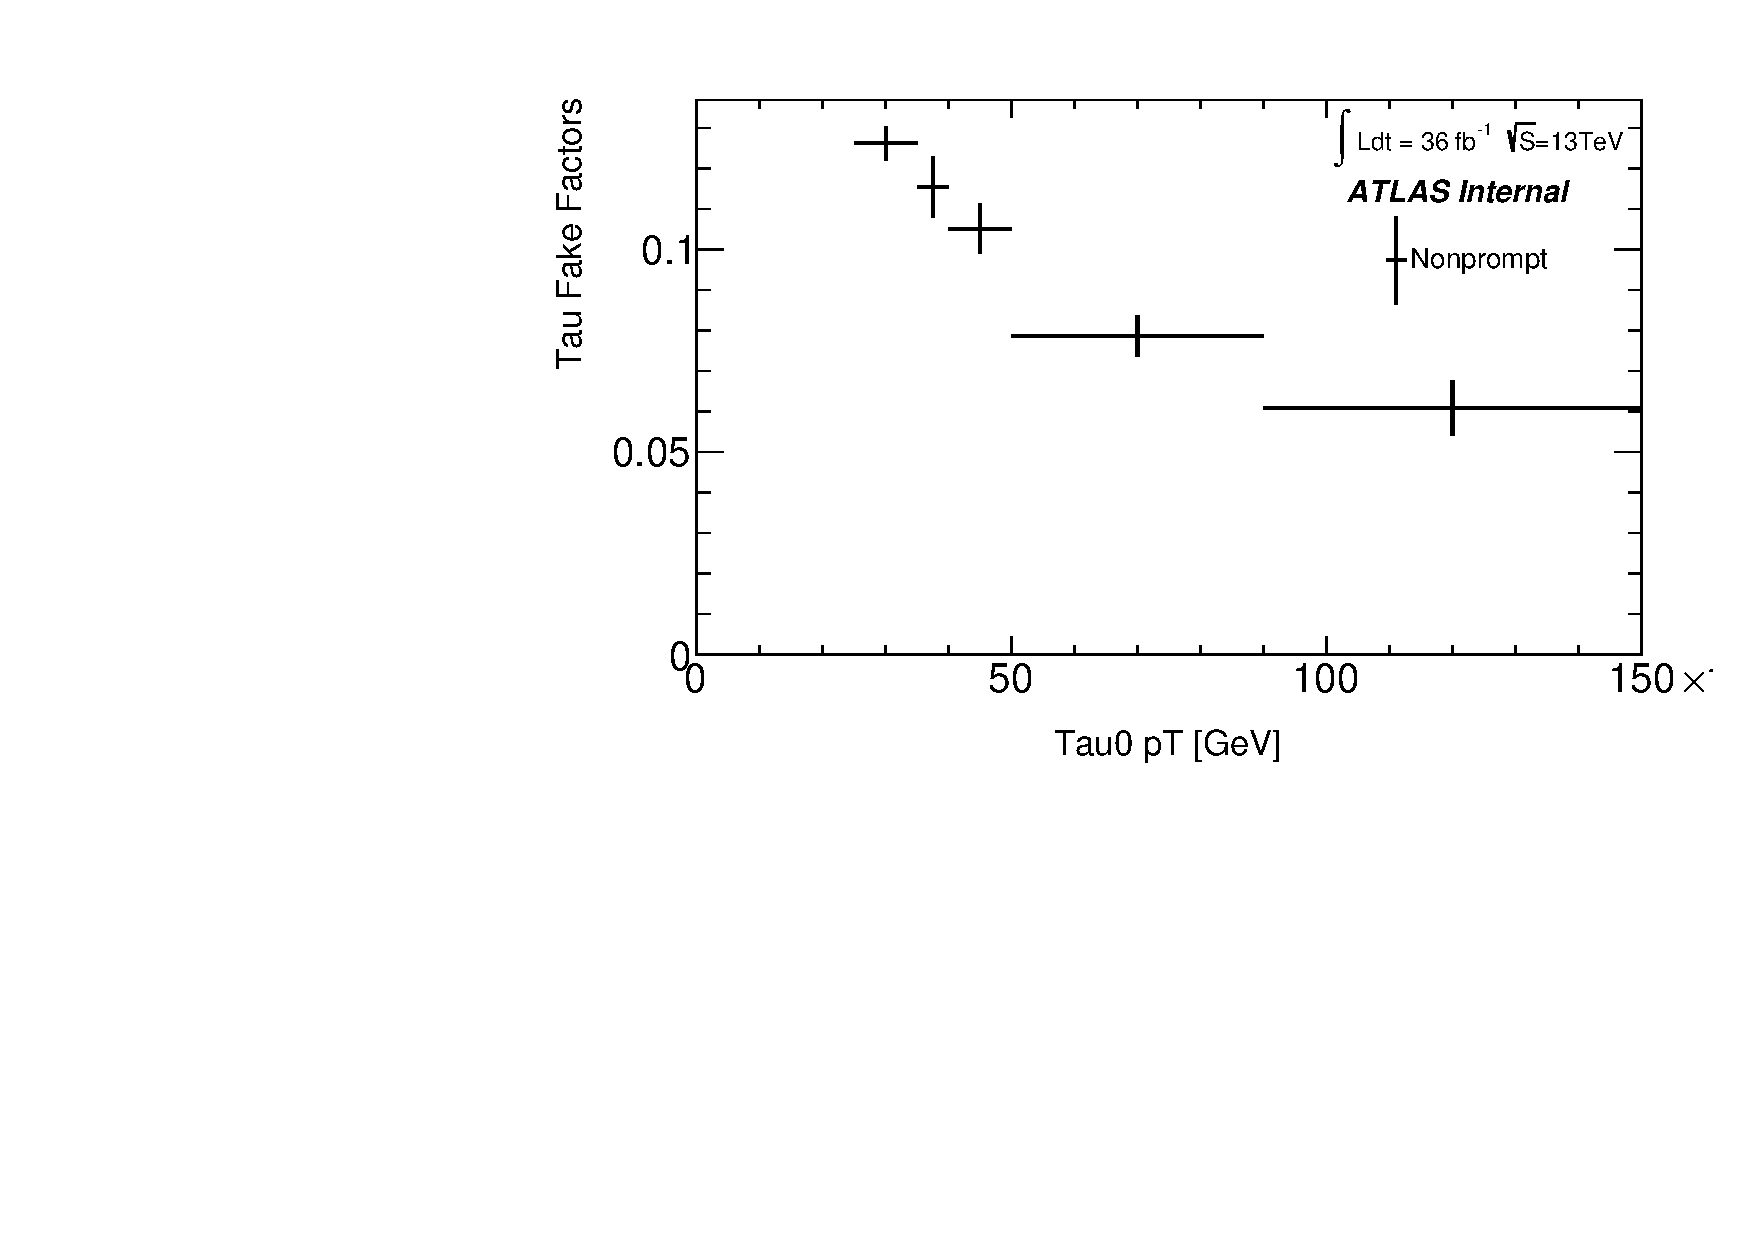
\includegraphics[width=0.95\linewidth]{figures/FakesEstimate_data_pp8_nonallhad_new_scaledHists/FF_Faketau_Nonprompt.pdf}
  	\caption{$p_T$-parametrized fake factors}
  	\label{fig:sub1}
	\end{subfigure}%
	\begin{subfigure}{.5\textwidth}
	\centering
	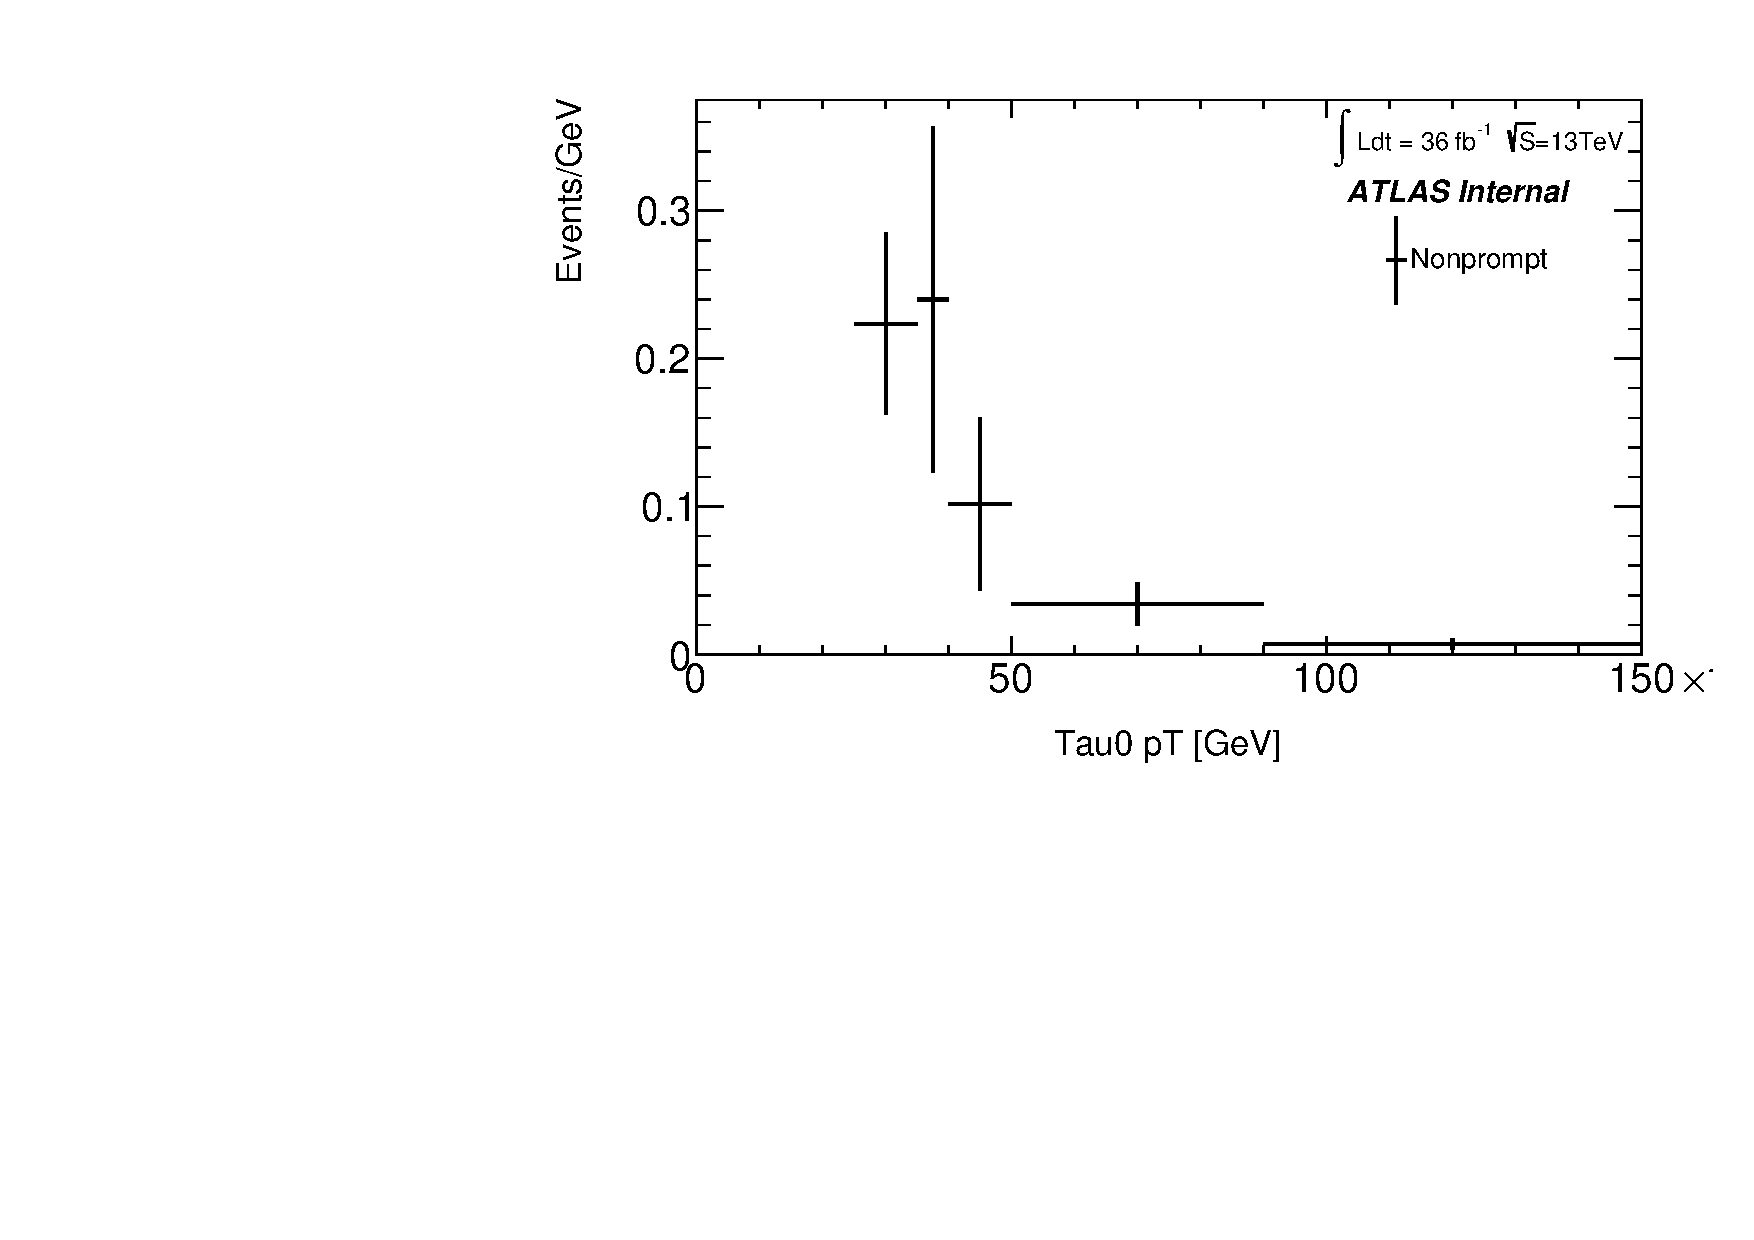
\includegraphics[width=0.95\linewidth]{figures/FakesEstimate_data_pp8_nonallhad_new_scaledHists/hist_Extrapolation_Nonprompt.pdf}
	\caption{Extrapolation sideband region $p_T$ spectrum}
	\end{subfigure}
	\caption{Fake factors and extrapolation sideband region, (Non-prompt MC)}
	\end{figure}
	
	\begin{figure}[H]
	\centering
	\begin{subfigure}{.5\textwidth}
	\centering
	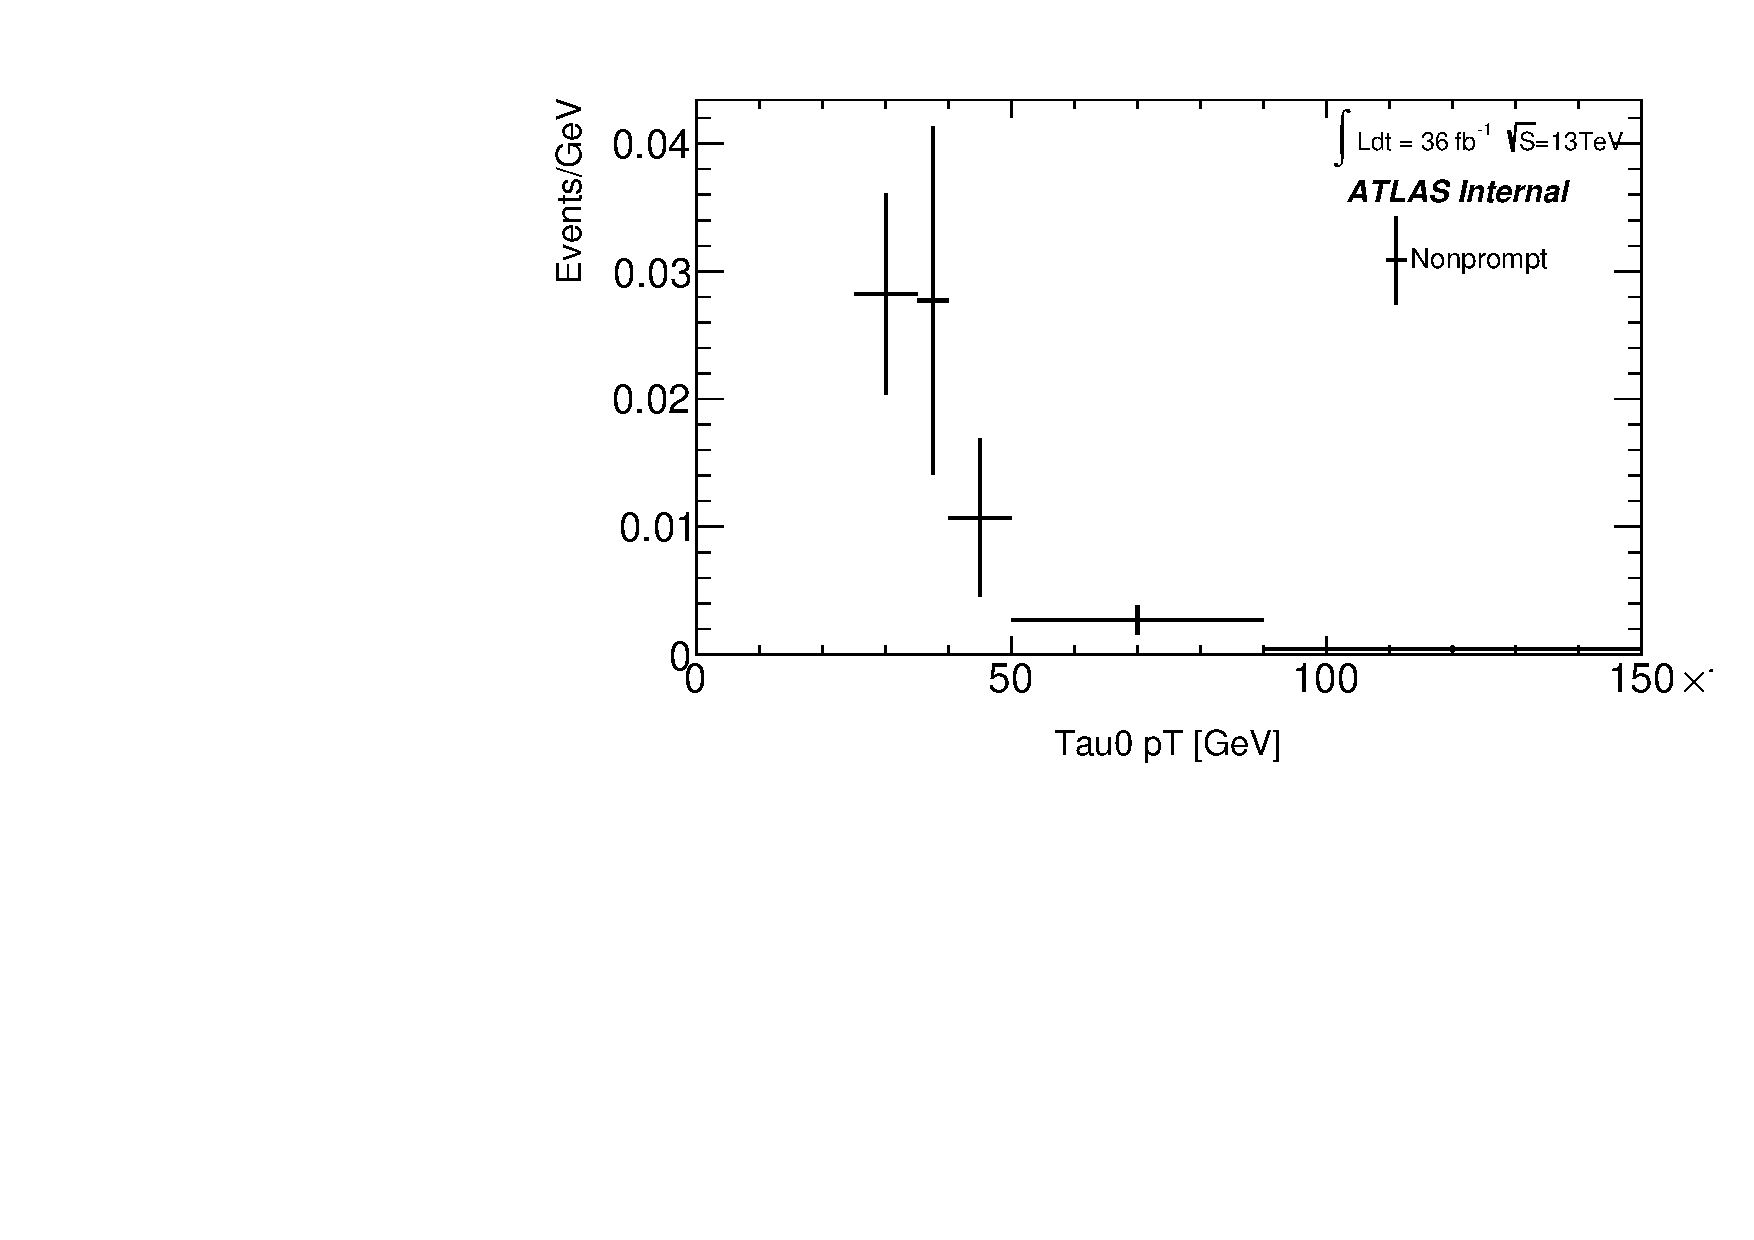
\includegraphics[width=0.95\linewidth]{figures/FakesEstimate_data_pp8_nonallhad_new_scaledHists/hist_FakeEstimate_Nonprompt.pdf}
  	\caption{Fake estimate in $p_T$ bins}
  	\label{fig:sub1}
	\end{subfigure}%
	\begin{subfigure}{.5\textwidth}
	\centering
	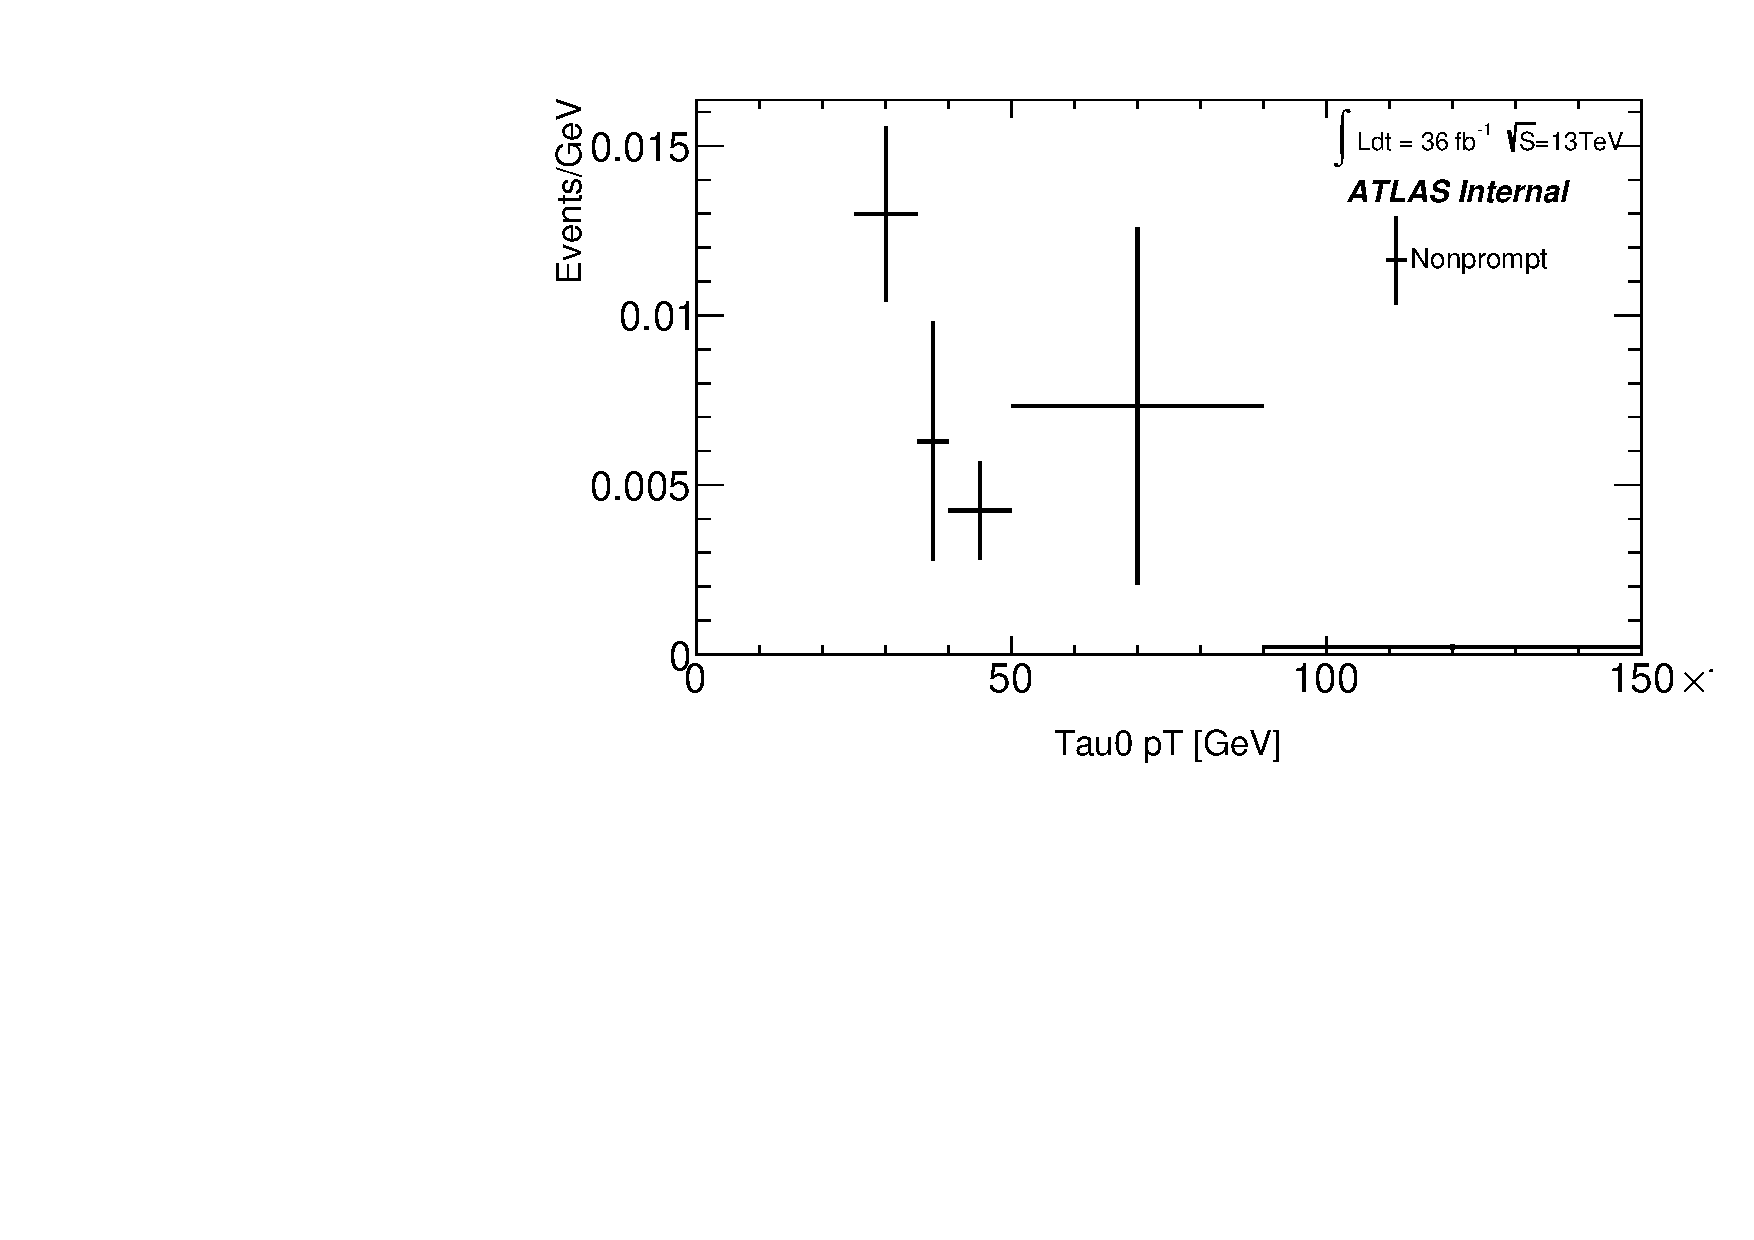
\includegraphics[width=0.95\linewidth]{figures/FakesEstimate_data_pp8_nonallhad_new_scaledHists/hist_SRMC_Nonprompt.pdf}
	\caption{MC SR yield in $p_T$ bins}
	\end{subfigure}
	\caption{$p_T$ spectra for fake estimate and MC yield, (Non-prompt MC)}
	\end{figure}

	\begin{figure}[H]
		\centering
		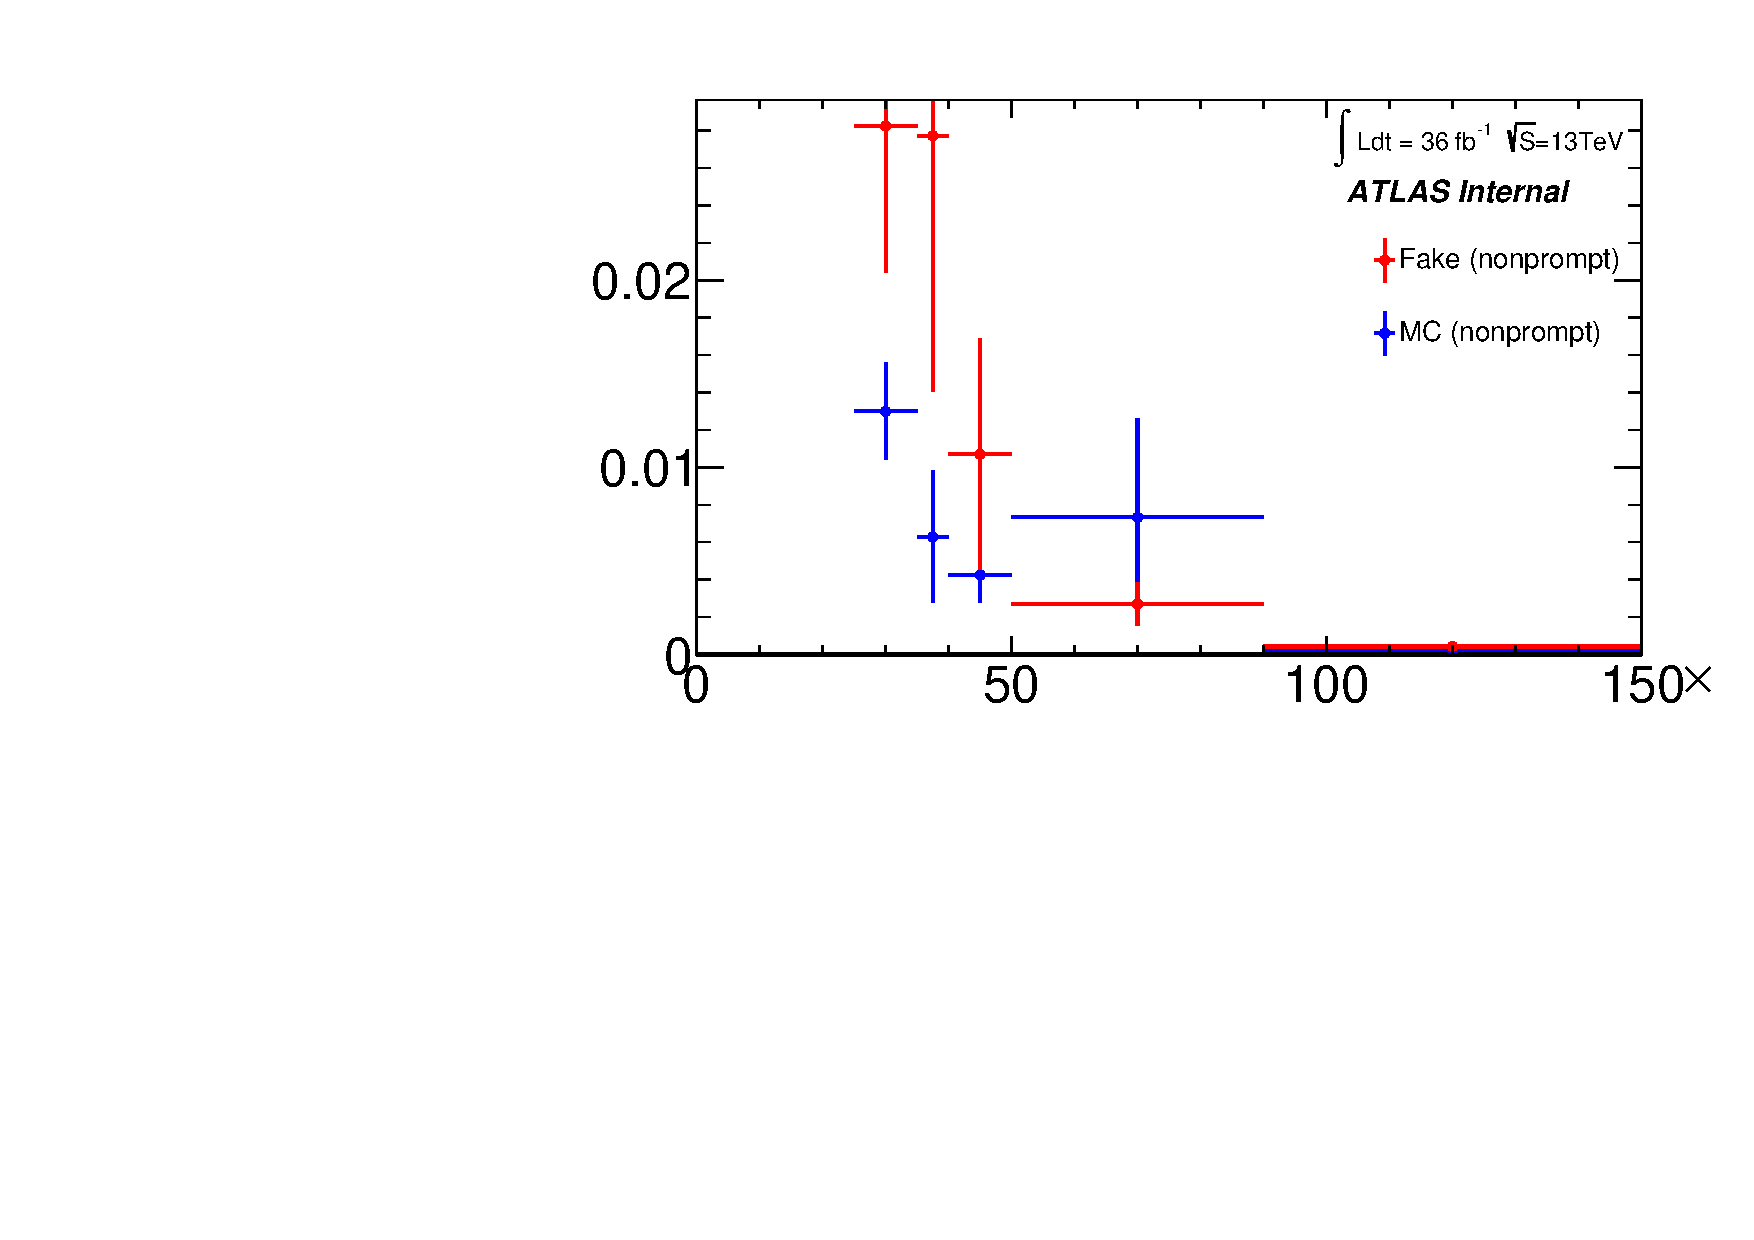
\includegraphics[width=0.7\linewidth]{figures/FakesEstimate_data_pp8_nonallhad_new_scaledHists/Overlay_FF_tau_pt_nonprompt.pdf}
		\caption{Overlaid fake estimate and MC prediction (Non-prompt MC)}
	\end{figure}	
		




	\clearpage
	\subsection{Estimate with prompt MC} 
	Here there is no subtraction performed and the estimate and closure test is done on the prompt MC only. 
	\begin{equation}
		FF(p_T)_{MC} = \frac{N_\tau (p_T)^{\text{Prompt MC}}}{N_{\cancel{\tau}} (p_T)^{\text{Prompt MC}}}
	\end{equation}

	\begin{table}[htp]
	\caption{Extrapolation and closure test, (Prompt MC)}
	\begin{center}
	\begin{tabular}{|c|c|c|}
	\hline
	Integrated fake estimate	& SR MC	& Closure \\
	\hline
	$1.71\pm0.26$ 		& $2.70\pm0.15$ 		& $58\pm25$\% \\
	\hline
	\end{tabular}
	\end{center}
	\label{default}
	\end{table}%
	
	A large difference between the fake estimate procedure and the MC prediction is seen at low $p_T$. If the lowest $p_T$ bin is omitted, the closure between the fake estimate ($1.41\pm0.16$) and the MC ($1.84\pm0.12$) improves to $30\pm18$\%. 
		
	\begin{figure}[H]
	\centering
	\begin{subfigure}{.5\textwidth}
	\centering
	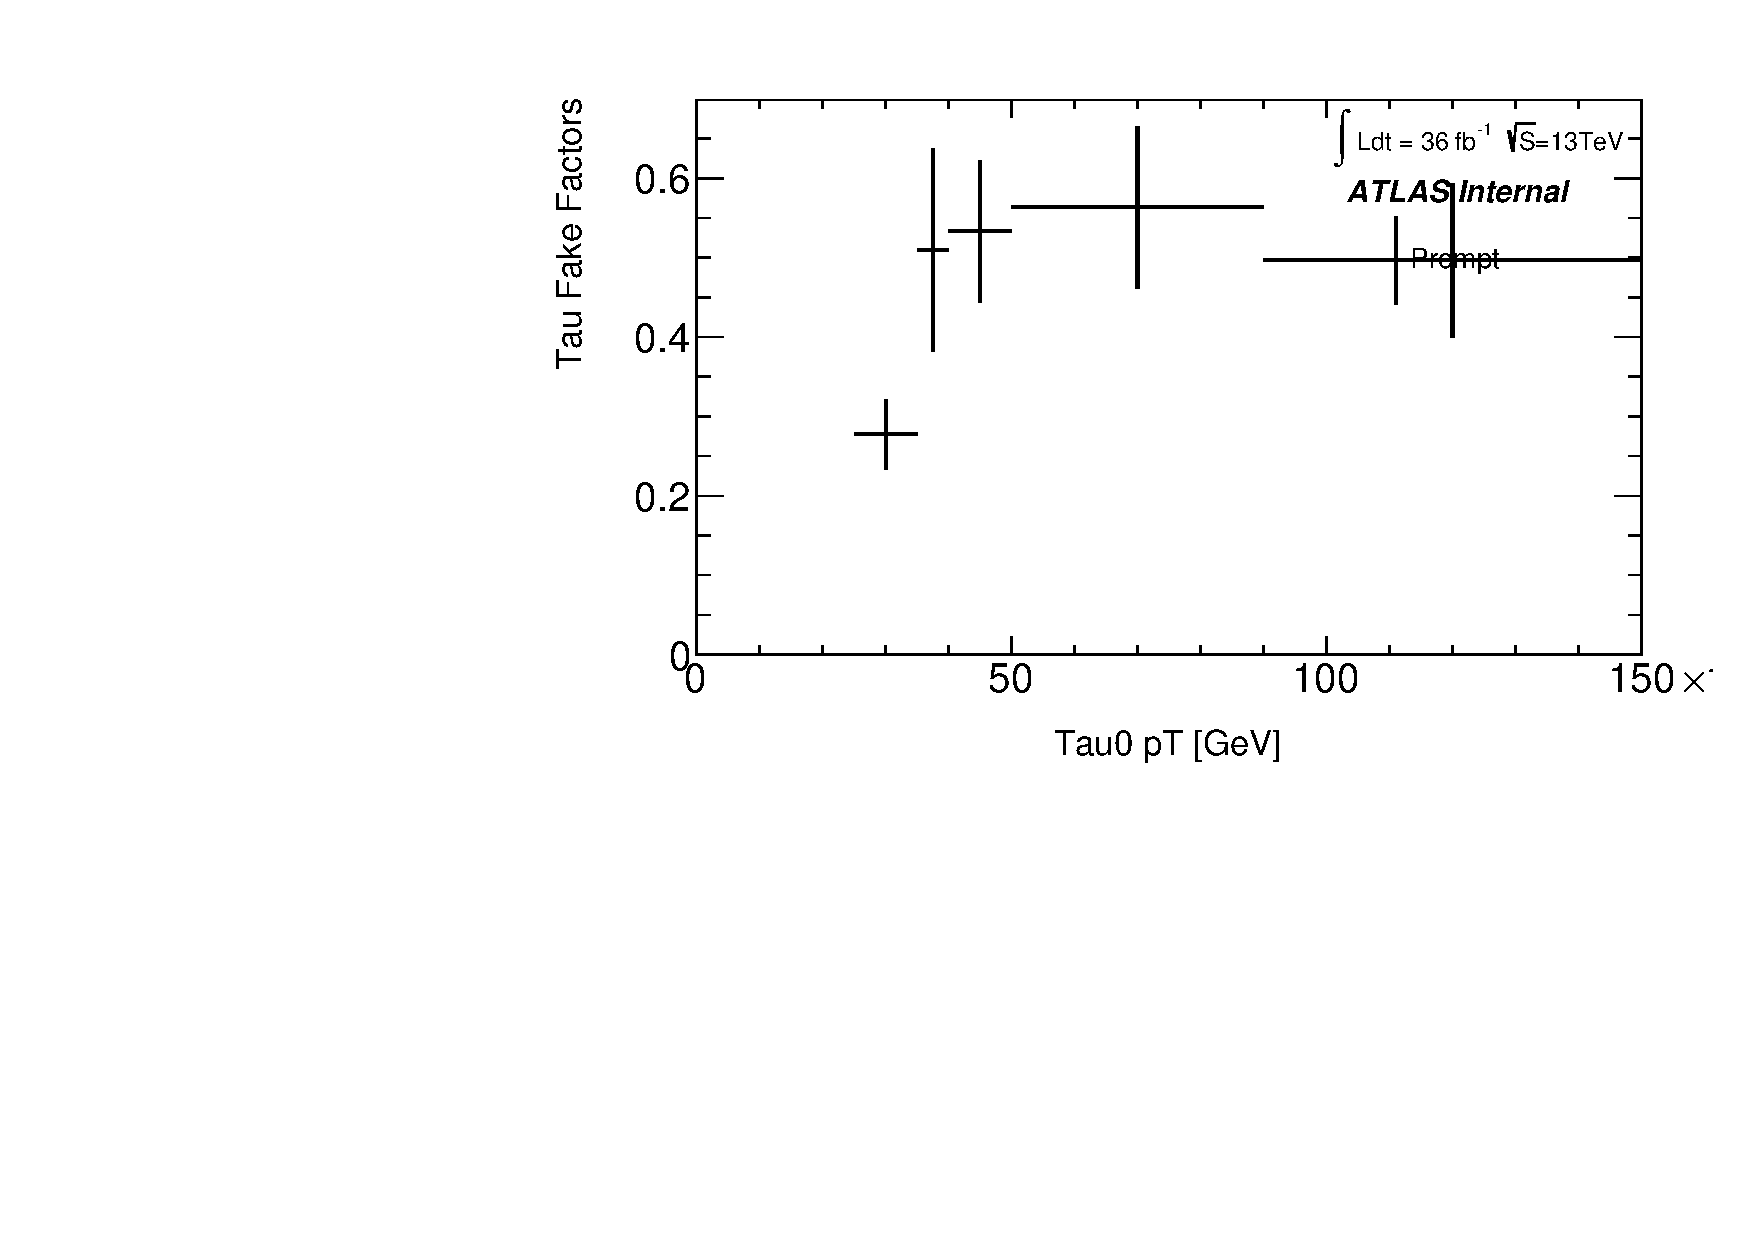
\includegraphics[width=0.95\linewidth]{figures/FakesEstimate_data_pp8_nonallhad_new_scaledHists/FF_Faketau_Prompt.pdf}
  	\caption{$p_T$-parametrized fake factors}
  	\label{fig:sub1}
	\end{subfigure}%
	\begin{subfigure}{.5\textwidth}
	\centering
	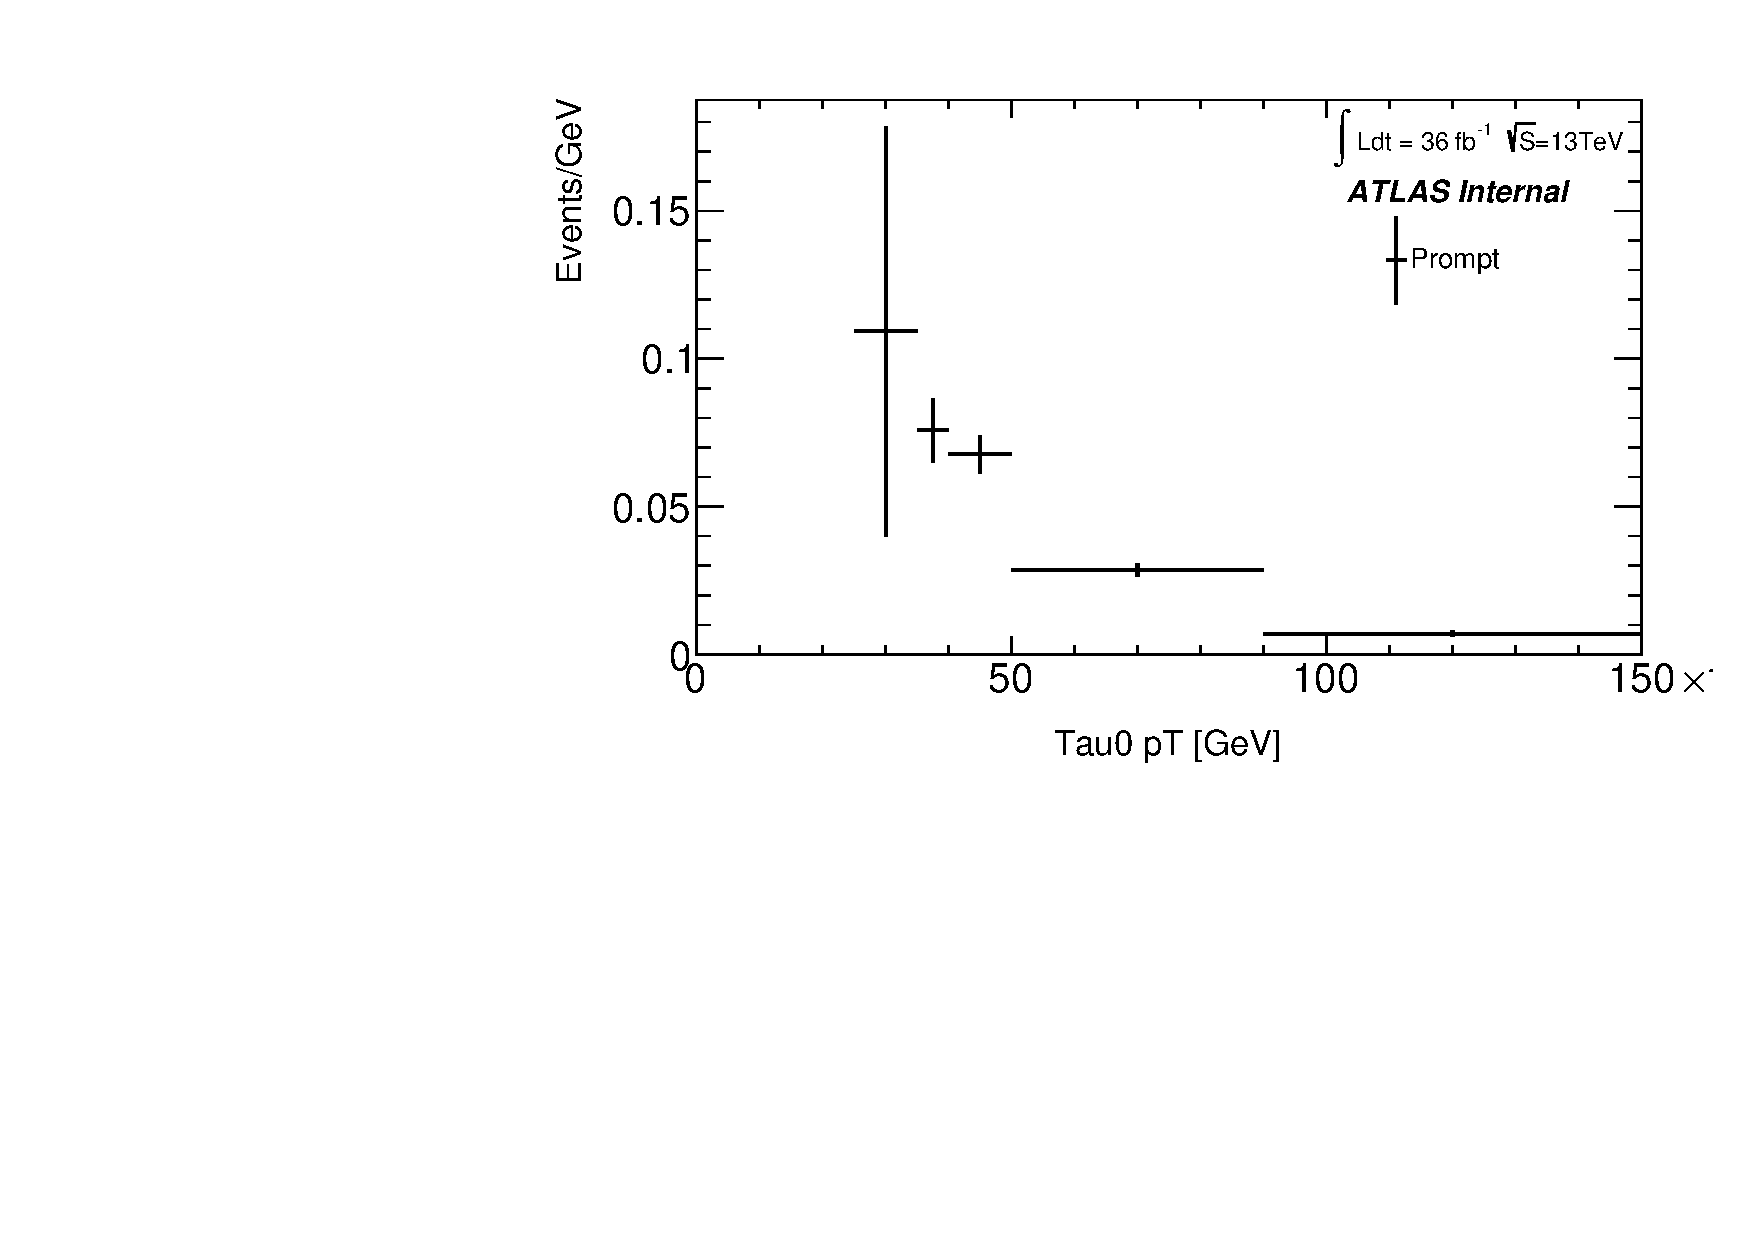
\includegraphics[width=0.95\linewidth]{figures/FakesEstimate_data_pp8_nonallhad_new_scaledHists/hist_Extrapolation_Prompt.pdf}
	\caption{Extrapolation sideband region $p_T$ spectrum}
	\end{subfigure}
	\caption{Fake factors and extrapolation sideband region, (Prompt MC)}
	\end{figure}
	
	\begin{figure}[H]
	\centering
	\begin{subfigure}{.5\textwidth}
	\centering
	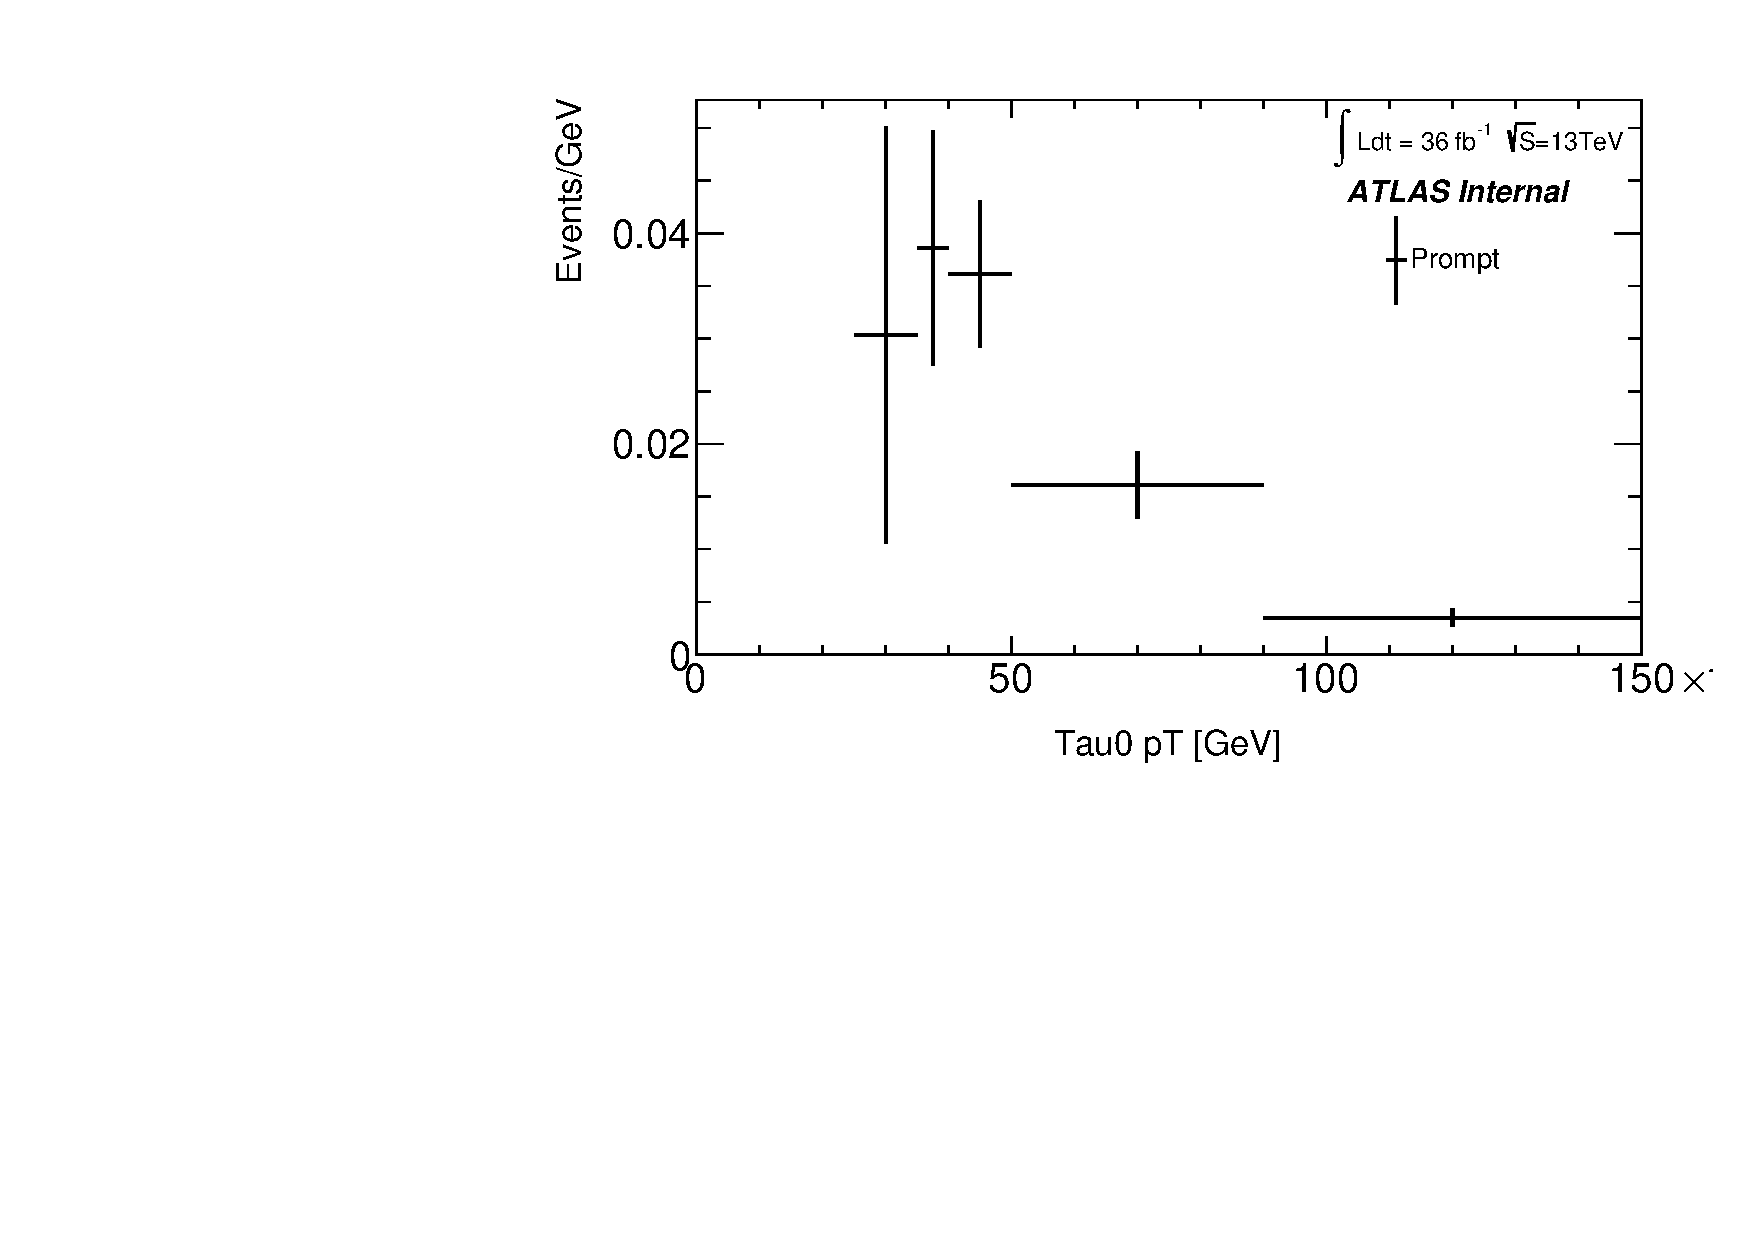
\includegraphics[width=0.95\linewidth]{figures/FakesEstimate_data_pp8_nonallhad_new_scaledHists/hist_FakeEstimate_Prompt.pdf}
  	\caption{Fake estimate in $p_T$ bins}
  	\label{fig:sub1}
	\end{subfigure}%
	\begin{subfigure}{.5\textwidth}
	\centering
	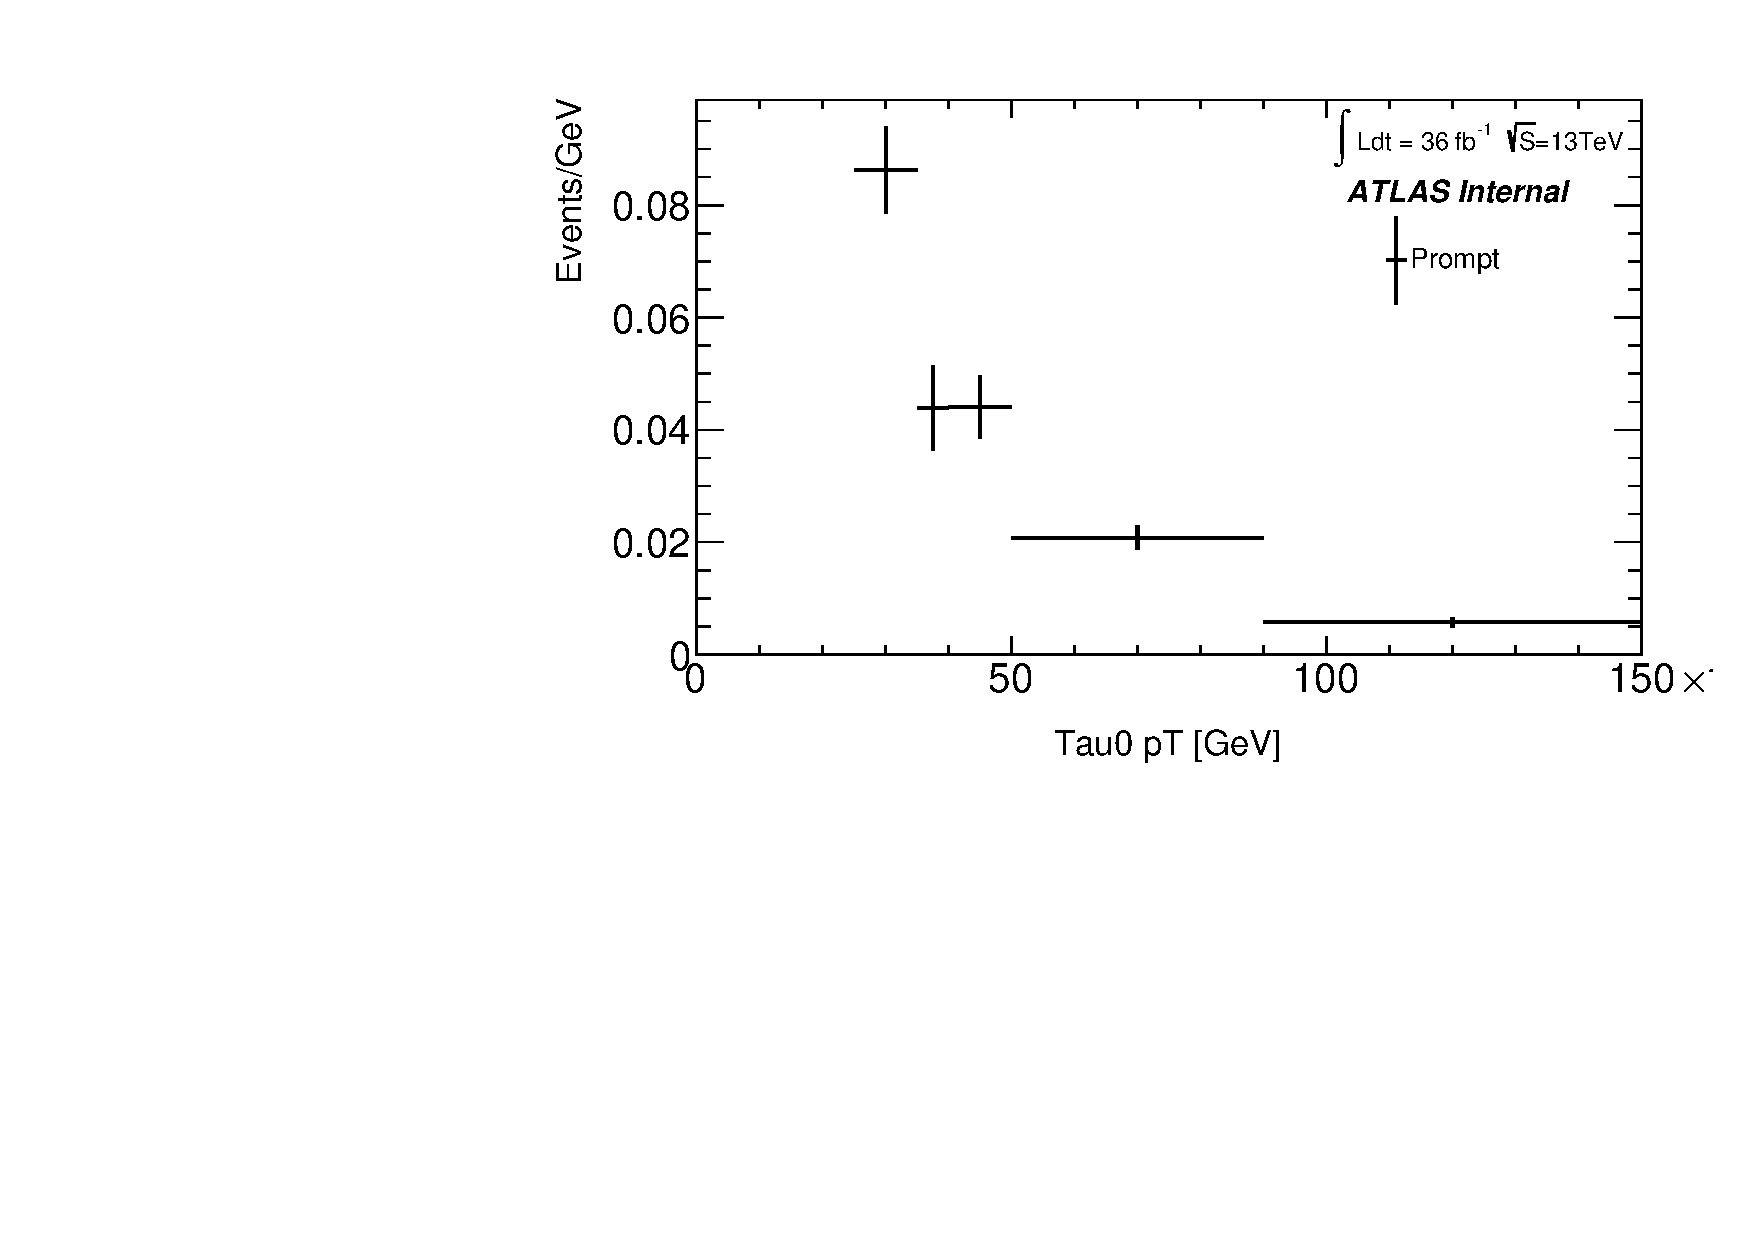
\includegraphics[width=0.95\linewidth]{figures/FakesEstimate_data_pp8_nonallhad_new_scaledHists/hist_SRMC_Prompt.pdf}
	\caption{MC SR yield in $p_T$ bins}
	\end{subfigure}
	\caption{$p_T$ spectra for fake estimate and MC yield, (Prompt MC)}
	\end{figure}

	\begin{figure}[H]
		\centering
		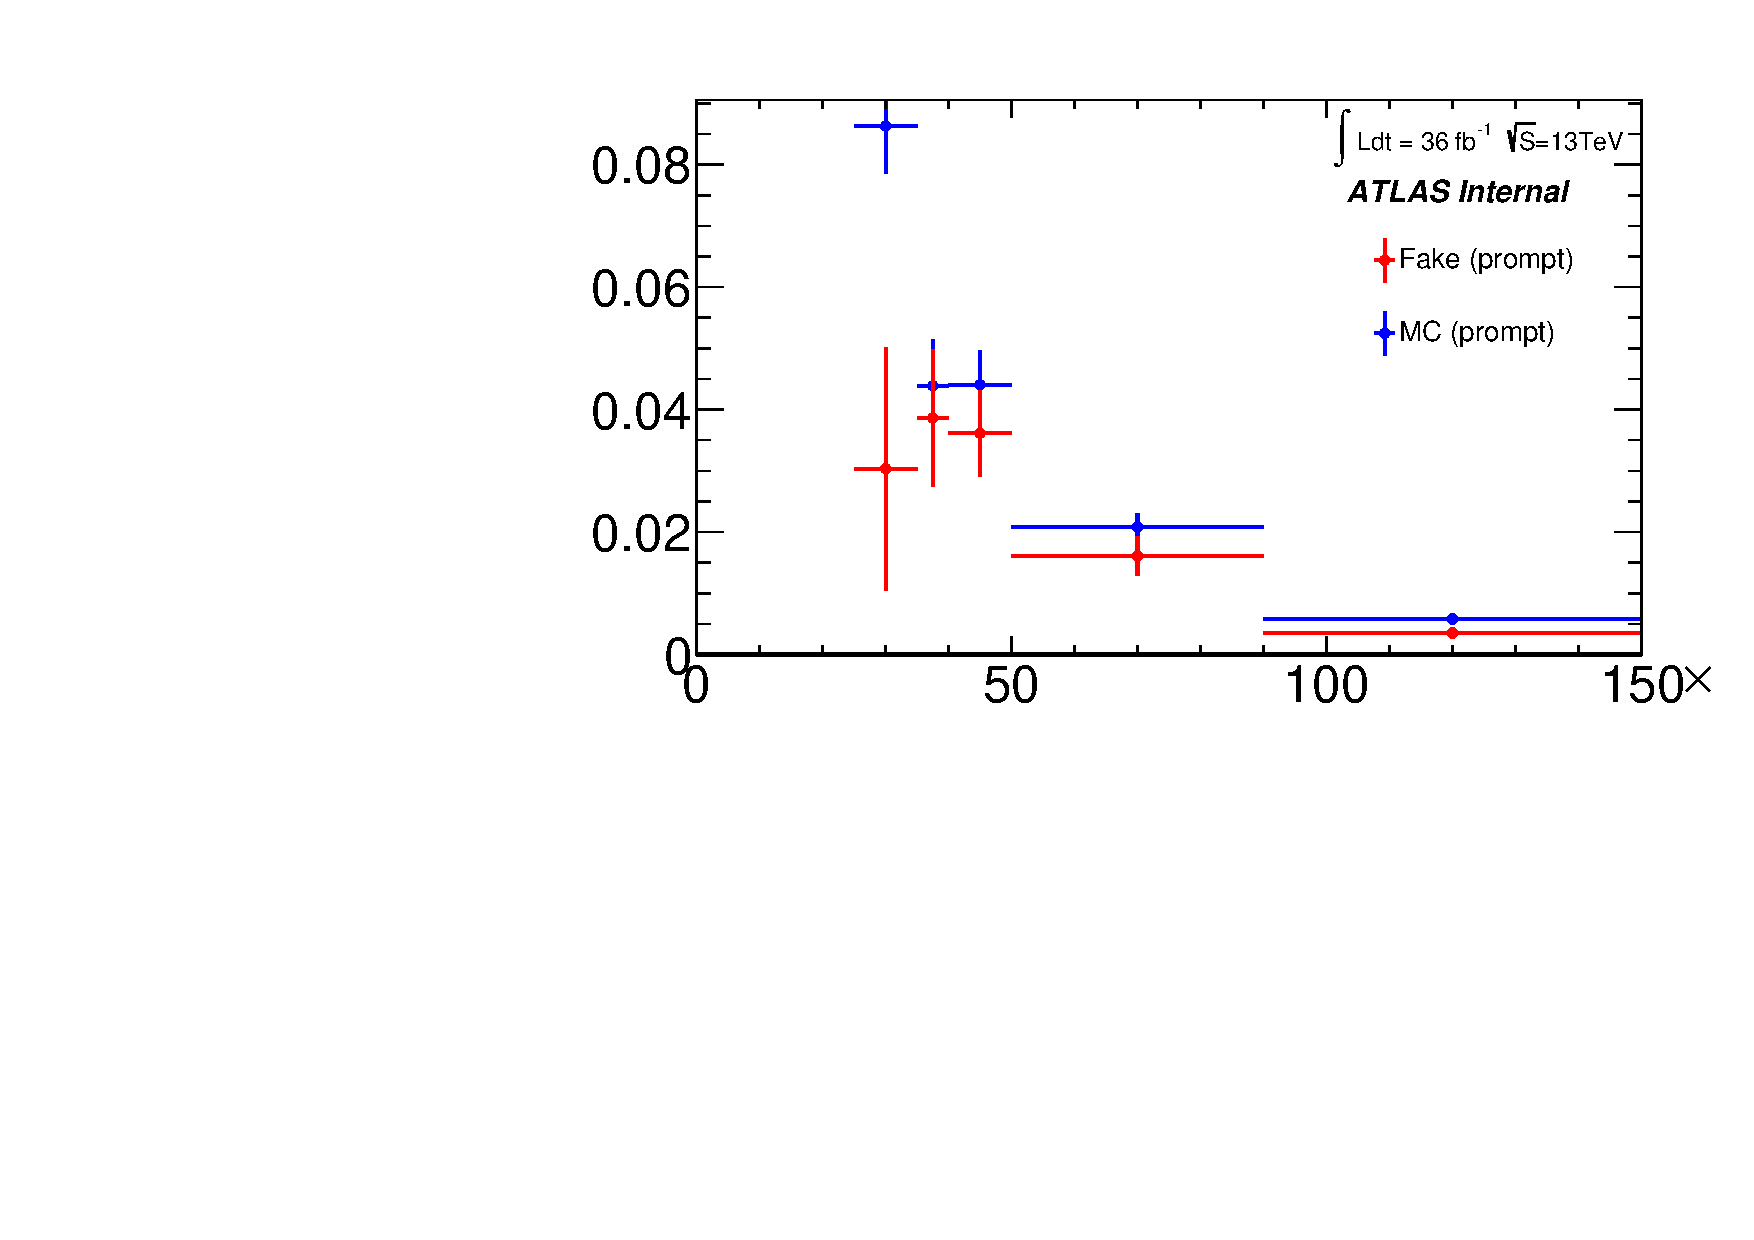
\includegraphics[width=0.7\linewidth]{figures/FakesEstimate_data_pp8_nonallhad_new_scaledHists/Overlay_FF_tau_pt_prompt.pdf}
		\caption{Overlaid fake estimate and MC prediction (Prompt MC)}
	\end{figure}	



	
	\clearpage
	\subsection{Data/MC comparison for $t\bar{t}$ samples in $2\ell OS+\tau$} 
	
	\begin{table}[htp]
	\caption{Data \& MC in $2\ell OS+\tau$ with different $t\bar{t}$ samples}
	\begin{center}
	\begin{tabular}{|c|c|c|c|c|c|}
	\hline
	$t\bar{t}$ sample 	& $t\bar{t}H$	& Prompt		& Nonprompt		& 	 Data 	& Data/MC\\
	\hline
	PP8 				& 	$2.467 \pm 0.080$ 		& $4.084 \pm 0.273$ 		& $924.376 \pm 28.516$	&  $951$ 	& $1.029$\\
	PP8 (high stats)		& 			''	 		&			''			& $920.071 \pm 21.203$	&  	''	& $1.034$\\
	PP8 (dilep) 			& 			''	 		& 			''			& $896.863 \pm 20.615$	&   	''	& $1.060$\\
	PP8 (dilep, high stats)	& 			''			& 			''	 		& $882.809 \pm 16.779$	&   	''	& $1.077$\\ 
	\hline
	\end{tabular}
	\end{center}
	\label{default}
	\end{table}%

	\begin{table}[htp]
	\caption{Data \& MC in $2\ell OS+\cancel{\tau}$ with different $t\bar{t}$ samples}
	\begin{center}
	\begin{tabular}{|c|c|c|c|c|c|}
	\hline
	$t\bar{t}$ sample 	& $t\bar{t}H$	& Prompt		& Nonprompt		& 	 Data	& Data/MC \\
	\hline
	PP8 				& 	$4.399 \pm 0.108$ 		& $9.589 \pm 0.608$ 		& $8664.639 \pm 76.760$	&  $8271$ & $0.954$\\
	PP8 (high stats)		& 			''	 		&			''			& $8647.666 \pm 59.076$	&  	''	  & $0.956$\\
	PP8 (dilep) 			& 			''	 		& 			''			& $8580.240 \pm 62.630$	&   	''	  & $0.964$\\
	PP8 (dilep, high stats)	& 			''			& 			''	 		& $8590.145 \pm 49.257$	&   	''	  & $0.963$\\ 
	\hline
	\end{tabular}
	\end{center}
	\label{default}
	\end{table}%
	

	\begin{figure}[H]
		\begin{subfigure}[b]{.5\textwidth}
			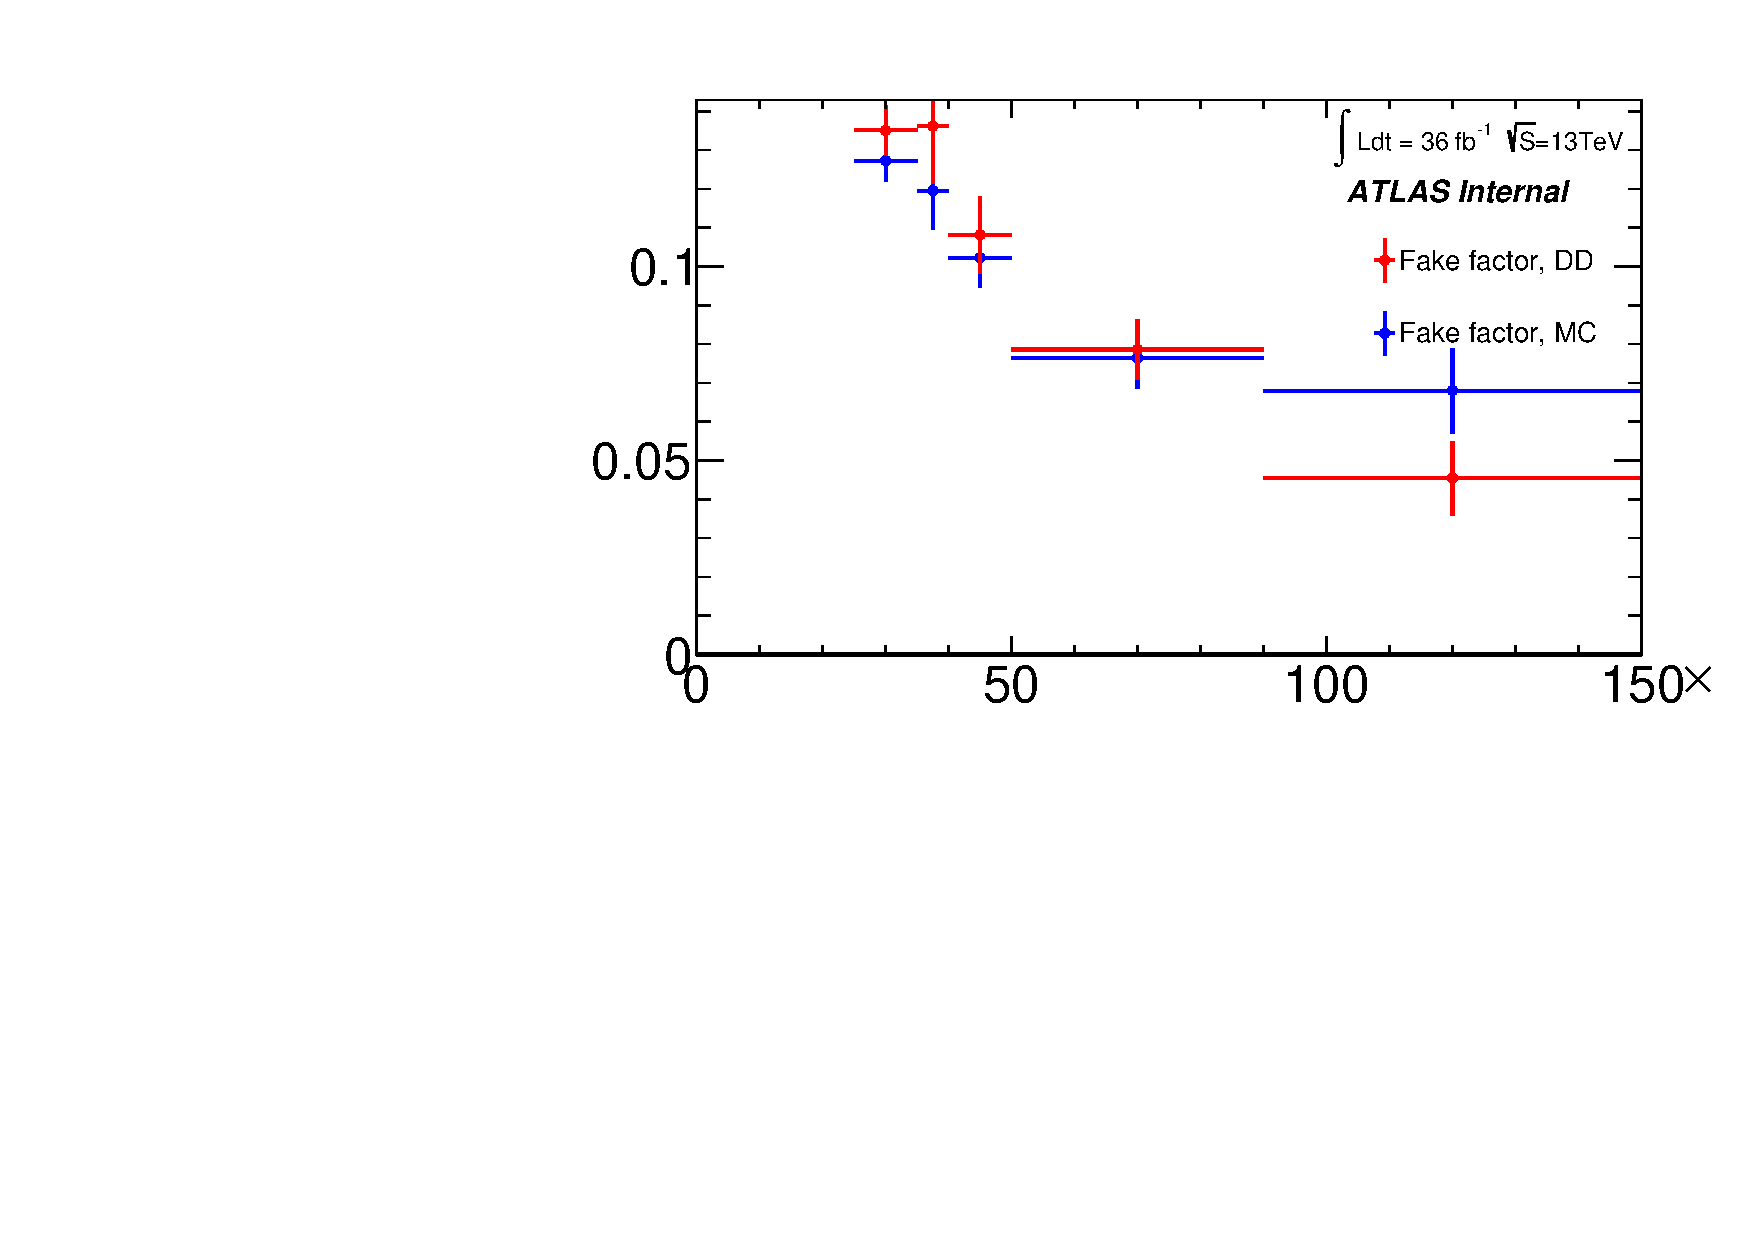
\includegraphics[width=0.82\linewidth]{figures/FakesEstimate_data_pp8_nonallhad_old/Overlay_FF_tau_pt_data.pdf}
  			\caption{PP8 $t\bar{t}$ non-allhad (410501)}
		\end{subfigure}
		\hfill
		\begin{subfigure}[b]{.5\textwidth}
			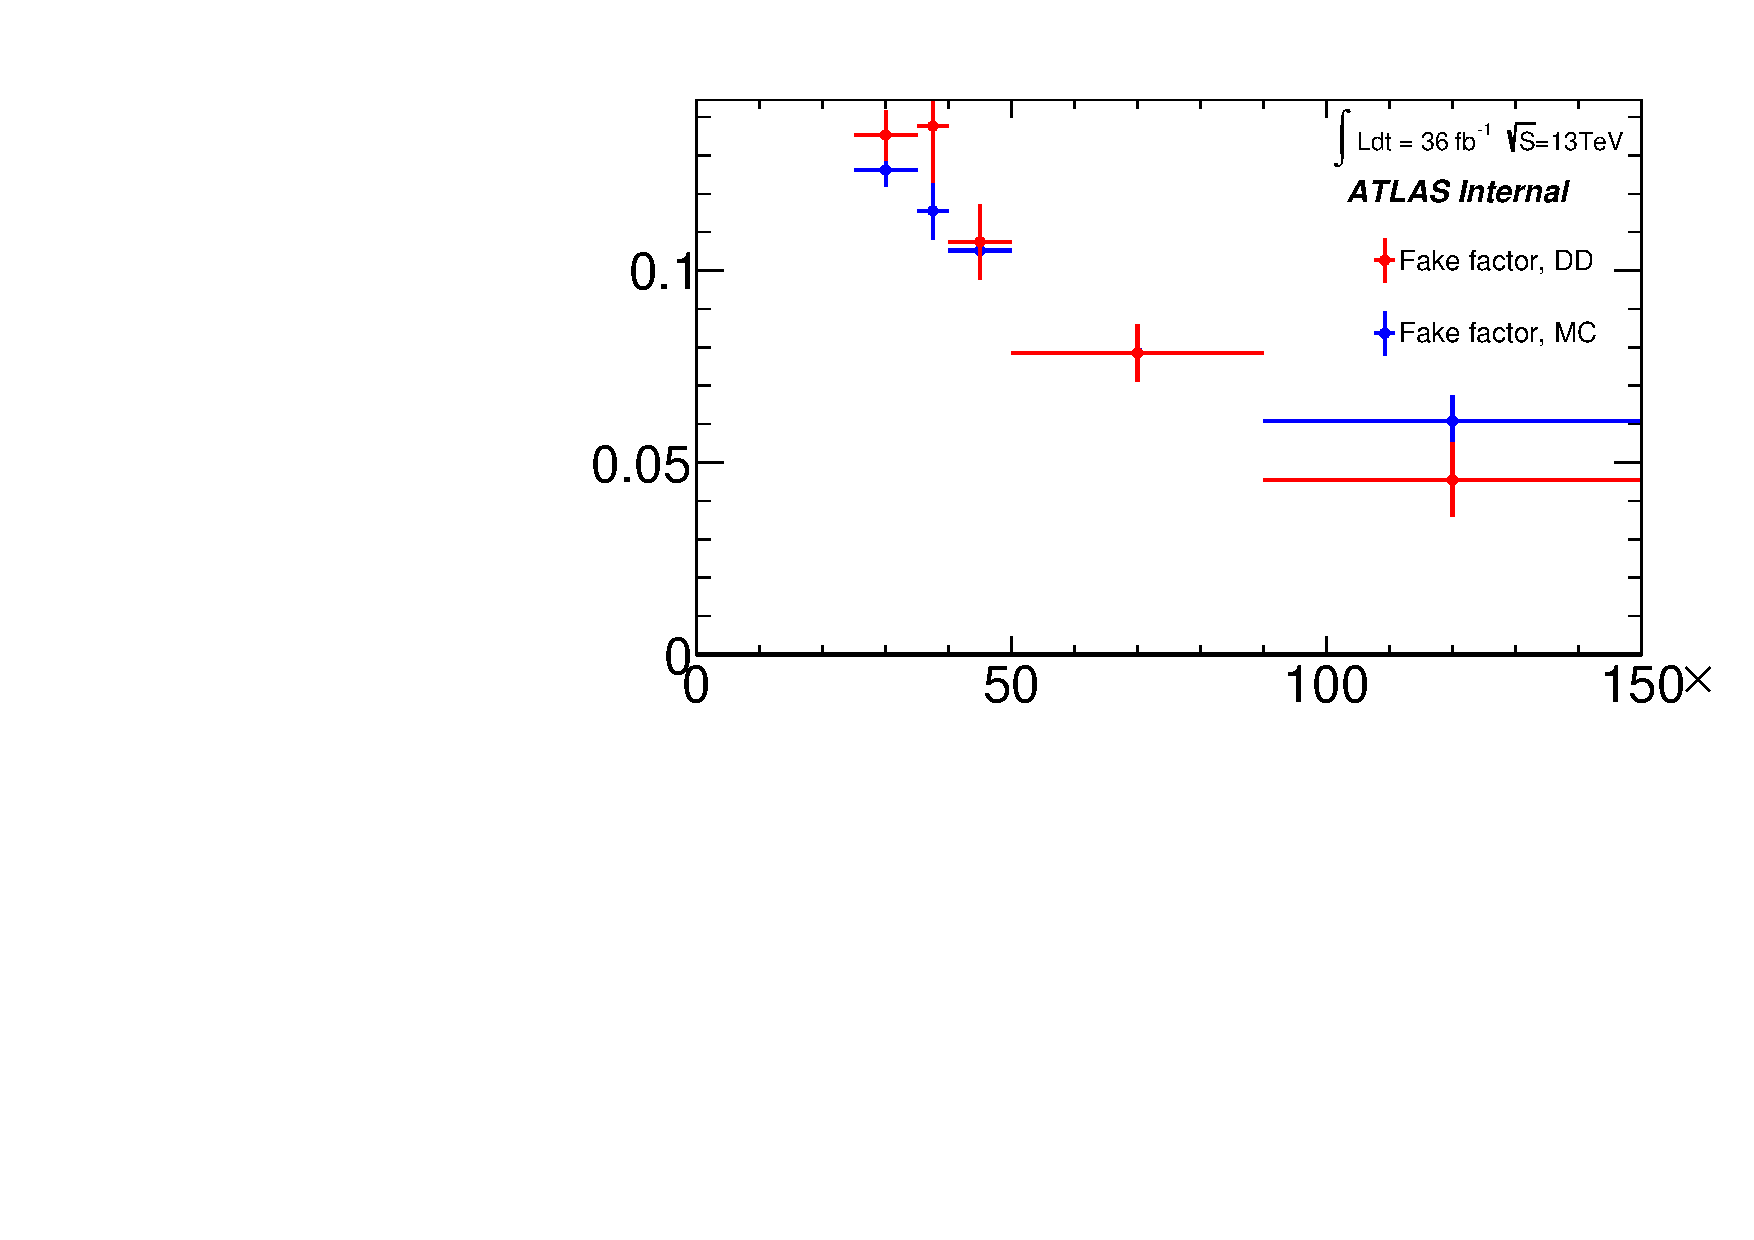
\includegraphics[width=0.82\linewidth]{figures/FakesEstimate_data_pp8_nonallhad_new/Overlay_FF_tau_pt_data.pdf}
			\caption{PP8 $t\bar{t}$ non-allhad (410501), high stats}
		\end{subfigure}%
		\vskip\baselineskip
		\begin{subfigure}[b]{.5\textwidth}
			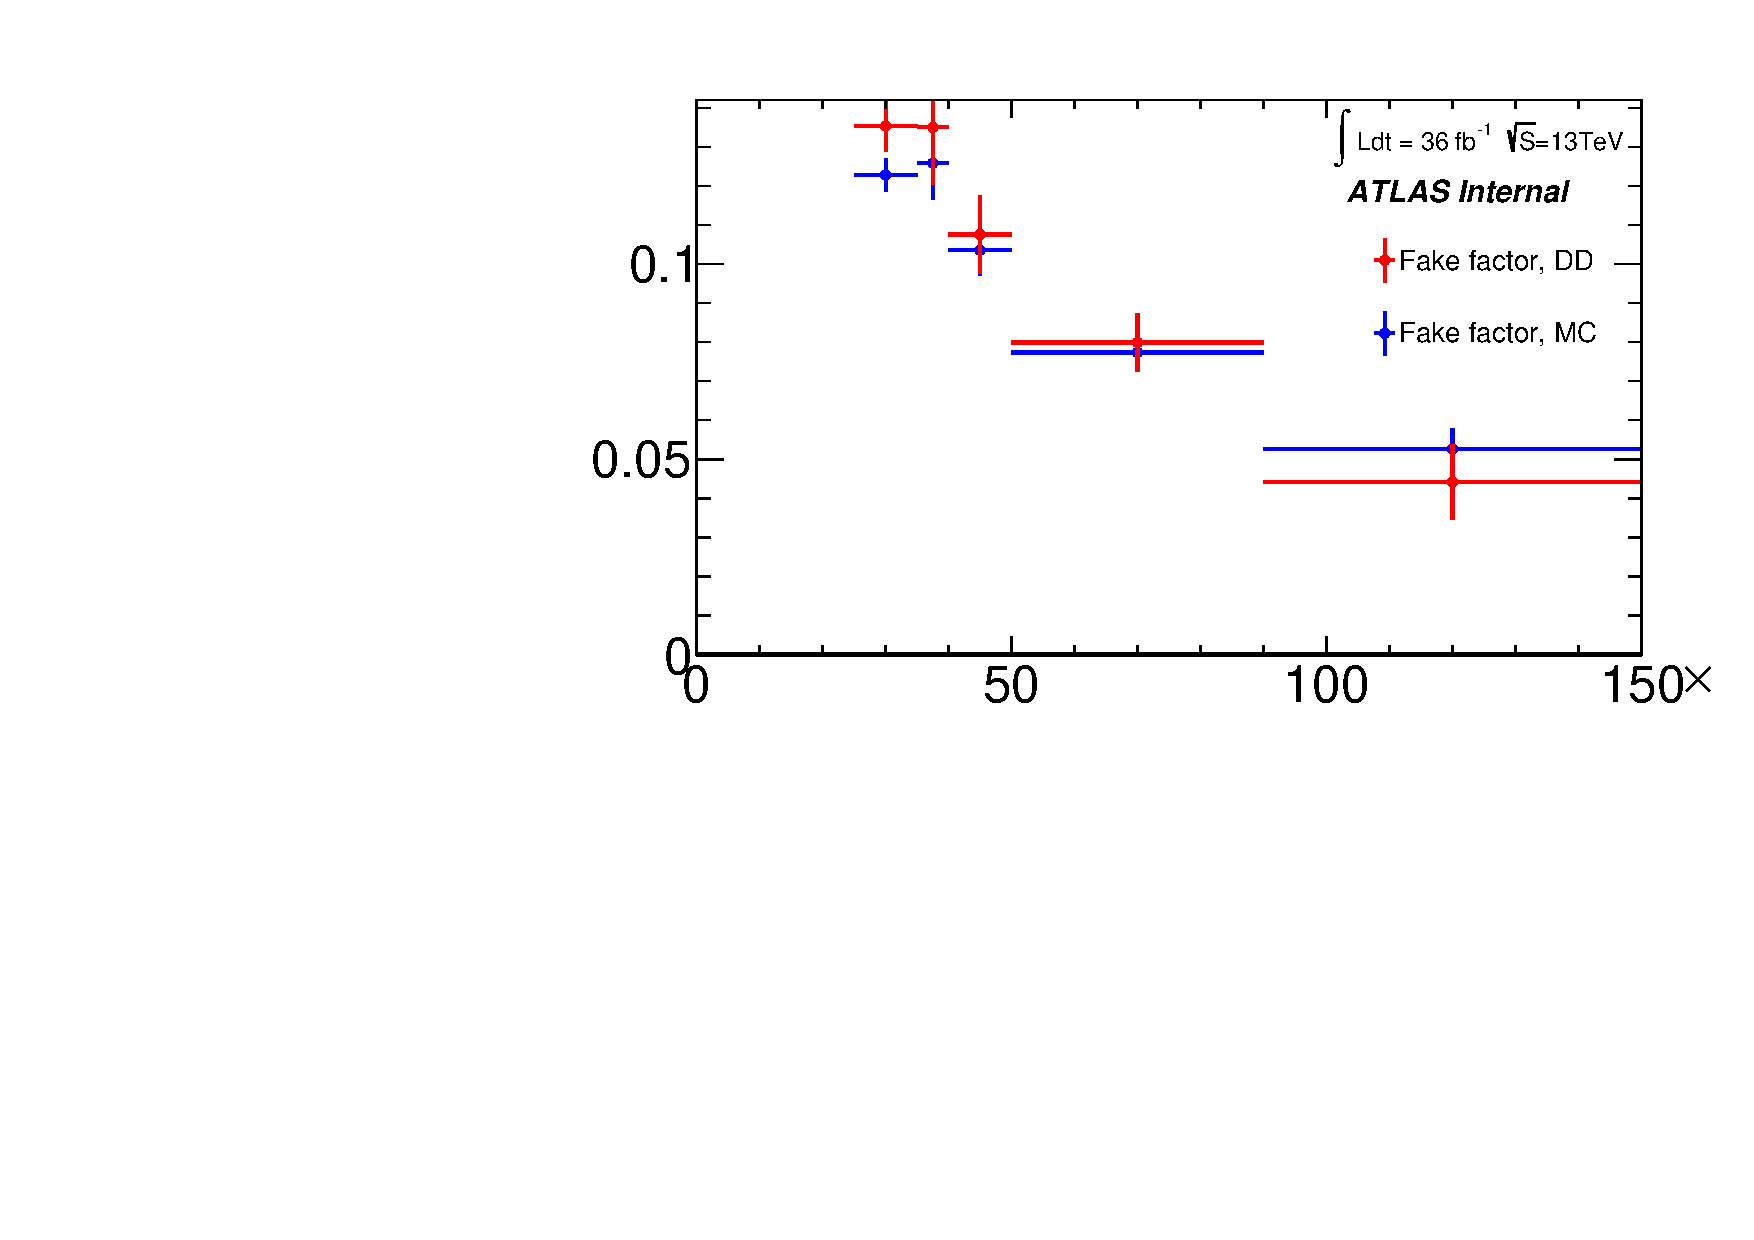
\includegraphics[width=0.82\linewidth]{figures/FakesEstimate_data_pp8_dilepton_old/Overlay_FF_tau_pt_data.pdf}
			\caption{PP8 $t\bar{t}$ dilepton (410503)}
		\end{subfigure}
		\quad
		\begin{subfigure}[b]{.5\textwidth}
			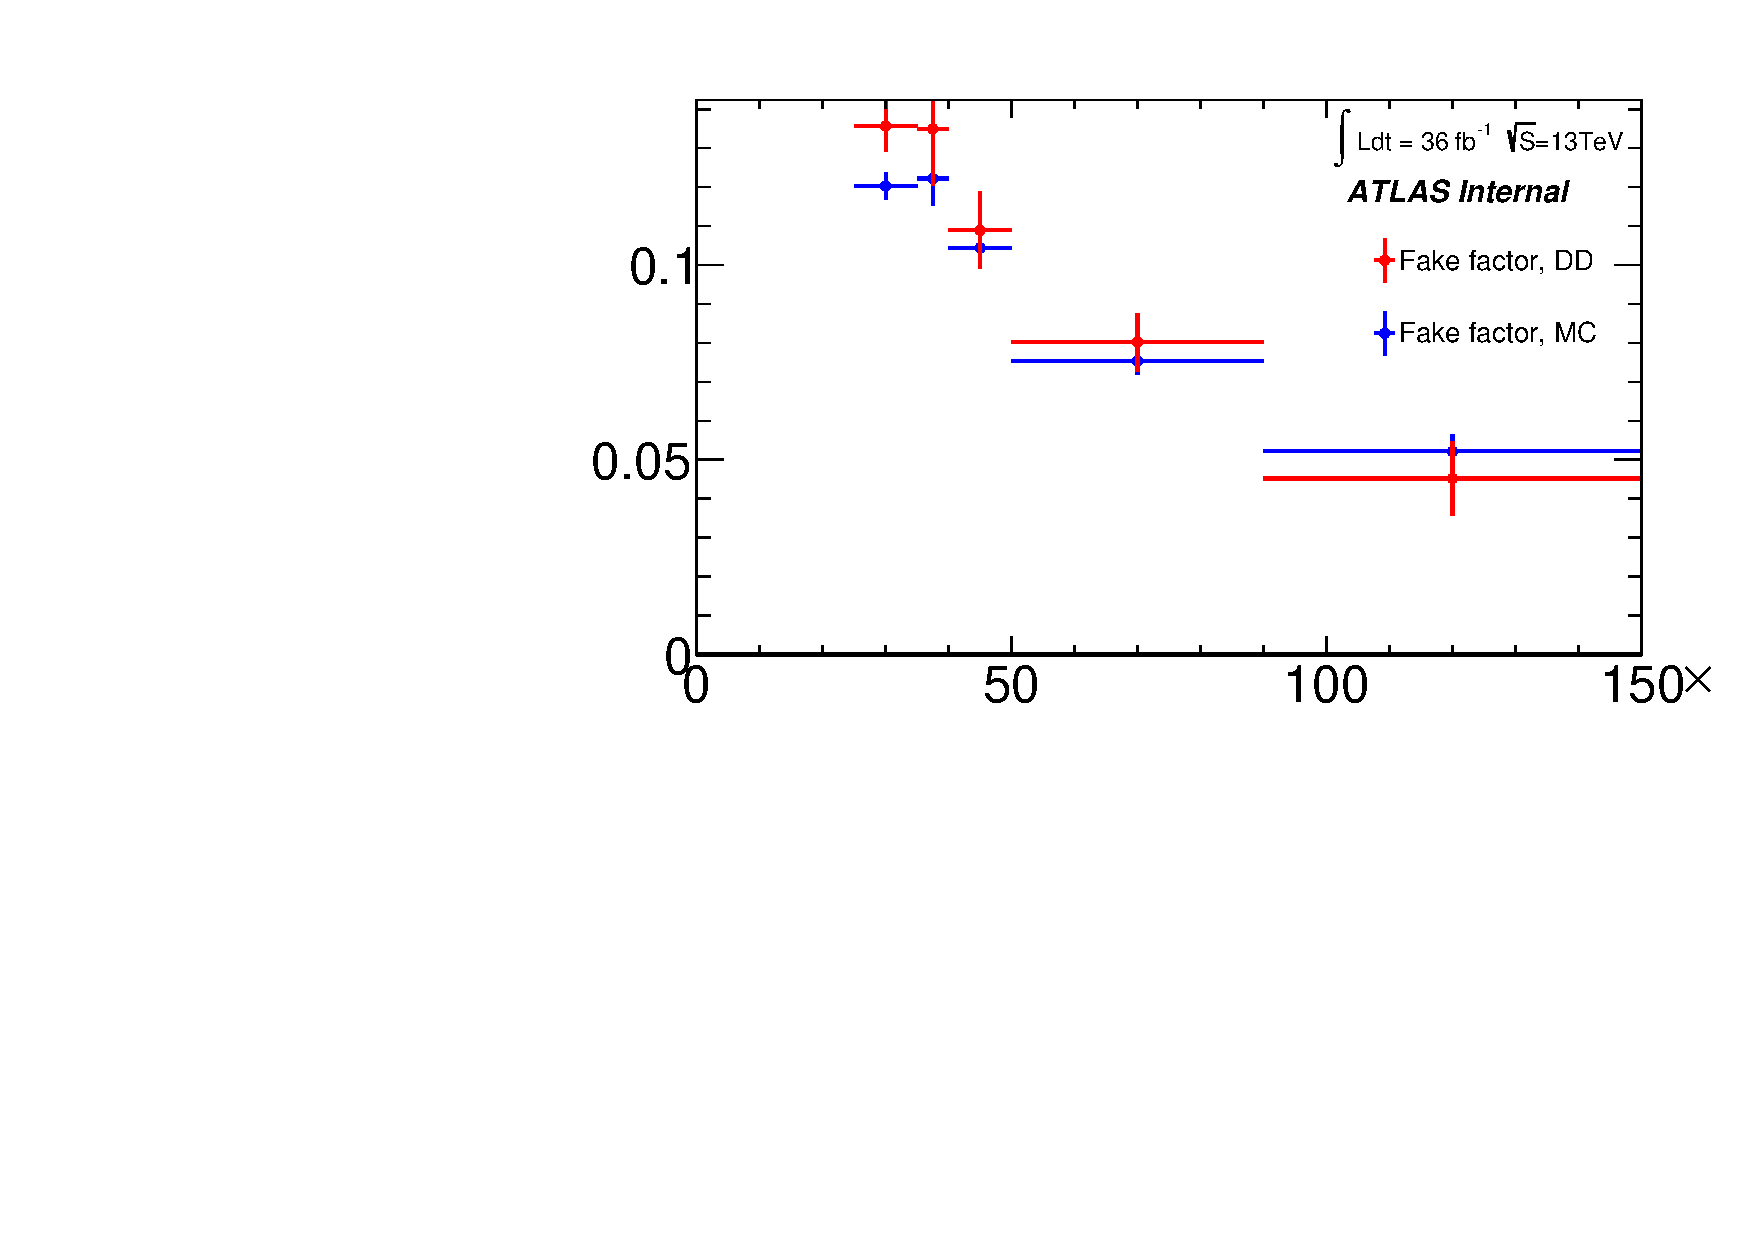
\includegraphics[width=0.82\linewidth]{figures/FakesEstimate_data_pp8_dilepton_new/Overlay_FF_tau_pt_data.pdf}
			\caption{PP8 $t\bar{t}$ dilepton (410503), high stats}
		\end{subfigure}
		\caption{MC fake factors compared with data}
	\end{figure}
	


	
	
	\clearpage
	\subsection{Data-driven estimate} 
	
	\clearpage
	\section{Ongoing to-do list} 
	\begin{itemize} 	
		\item Check results with new higher-stats $t\bar{t}$ samples, dilep-filtered samples and $t\bar{t}\gamma$ overlap samples
		\item Look into possible problem with calculation of weights/errors 
		\item Get fit framework running (see David Hohn) w. systematics ntuples 
		\item \textcolor{green}{DONE:} Validate data yields between vector- and flat-branch ntuple versions 
	\end{itemize} 
	
	
	\clearpage
	\section{Object selection}
	
	\clearpage
	\section{Event selection} 
		Signal region event selection:
		\begin{enumerate}
			\item Exactly 3 light leptons
			\item At least 1 trigger-matched light lepton 
			\item Low-mass dilepton invariant mass cut ($m\ell\ell>12$ GeV) 
			\item Z-mass dilepton invariant mass veto (Z mass = $91.2$ GeV with $10$ GeV window) 
			\item Exactly 1 hadronic tau 
			\item Total light lepton + hadronic tau charge == 0 
			\item At least 2 jets
			\item At least 1 b-tagged jet
		\end{enumerate} 

	

	
	\end{document} 



